\documentclass[11pt,letterpaper]{article}
% Adapted from docs/research_raw/paper_rewrite_2026-11-10/integrated/preamble.tex
% (sha256 195f9be4...ed8). Fonts, transcript-card box and quote macros are kept;
% incident macros, the fact lookup and the prompt box are new in this draft.
\usepackage[margin=0.95in,headheight=14pt]{geometry}
\usepackage{fontspec}
\setmainfont{TeX Gyre Pagella}
\setsansfont{TeX Gyre Heros}
\setmonofont[Scale=0.85]{Latin Modern Mono}
\newfontfamily\transcriptfont{TeX Gyre Heros}[RawFeature=-tlig]
\usepackage{microtype,graphicx,booktabs,tabularx,longtable,array,amsmath,amssymb}
\usepackage{enumitem,caption,xcolor,xurl,placeins,float}
\usepackage[most]{tcolorbox}
\usepackage{needspace}
\usepackage[numbers,sort&compress]{natbib}
\usepackage[colorlinks=true,linkcolor=blue!40!black,citecolor=blue!40!black,urlcolor=blue!40!black]{hyperref}
\graphicspath{{assets/}}
\setlength{\parskip}{3pt plus 1pt}
\setlength{\emergencystretch}{2em}
\setlist{itemsep=2pt,topsep=4pt,leftmargin=1.6em}
\captionsetup{font=small,labelfont=bf}
\newcolumntype{Y}{>{\raggedright\arraybackslash}X}
\newcolumntype{L}[1]{>{\raggedright\arraybackslash}p{#1}}
\newcommand{\game}[1]{G#1}
\newcommand{\artifact}[1]{\path{#1}}
\newcommand{\tablenote}[1]{\par\smallskip{\footnotesize #1}\par}
% Transcript cards. Quotation text and metadata are generated from canonical
% decision records by analysis/build_quotes.py; surrounding prose is authored.
\definecolor{transcriptbg}{HTML}{F4F5F6}
\definecolor{transcriptborder}{HTML}{D9DDE1}
\definecolor{transcriptmeta}{HTML}{50575E}
\newtcolorbox{transcriptmessage}{enhanced,colback=transcriptbg,
  colframe=transcriptborder,boxrule=0.45pt,arc=2.5mm,
  left=10pt,right=10pt,top=6pt,bottom=7pt,
  before skip=5pt,after skip=5pt,
  fontupper=\transcriptfont\fontsize{10}{13.2}\selectfont\raggedright,
  before upper={\hyphenpenalty=10000\exhyphenpenalty=10000}}
\newcommand{\DeclareTranscriptQuote}[3]{%
  \expandafter\gdef\csname transcript@#1\endcsname{%
    \begin{transcriptmessage}
    {\color{transcriptmeta}\fontsize{8.5}{11}\selectfont #2\par}
    \smallskip #3
    \end{transcriptmessage}}}
\newcommand{\TranscriptQuote}[1]{\ifcsname transcript@#1\endcsname\csname transcript@#1\endcsname\else\PackageError{quotes}{Undefined quote: #1}{}\fi}
\newcommand{\DeclareInlineQuote}[2]{\expandafter\gdef\csname inlinequote@#1\endcsname{#2}}
\newcommand{\InlineQuote}[1]{\ifcsname inlinequote@#1\endcsname ``{\transcriptfont\small\csname inlinequote@#1\endcsname}''\else\PackageError{quotes}{Undefined inline quote: #1}{}\fi}
\newcounter{incident}
\newcommand{\IncidentTitle}[2]{\par\FloatBarrier\addvspace{1.0em}\Needspace{11\baselineskip}%
  \refstepcounter{incident}\label{inc:#1}%
  \noindent{\large\bfseries Incident \theincident. #2}\par\smallskip}
\newcommand{\IncidentOutcome}[1]{\par\smallskip\noindent\textbf{Outcome.} #1\par}
\newcommand{\IncidentReading}[1]{\par\smallskip\noindent\textbf{Reading.} #1\par}
\newcommand{\IncidentSource}[1]{\par\smallskip{\footnotesize\color{transcriptmeta}#1}\par}
\newtcolorbox{promptbox}[1][]{enhanced,breakable,colback=white,colframe=transcriptborder,boxrule=0.45pt,arc=1mm,
  left=8pt,right=8pt,top=5pt,bottom=5pt,before skip=6pt,after skip=6pt,
  fontupper=\ttfamily\fontsize{8.6}{10.6}\selectfont\raggedright,#1}

\hypersetup{pdftitle={LLM Agents Withhold a Rival's Monopoly Until They Need the Cash},pdfauthor={MonopolyBench project}}
\title{LLM Agents Withhold a Rival's Monopoly\\Until They Need the Cash\\[4pt]
\large Bargaining, liquidity and default in twenty games of Monopoly}
\author{MonopolyBench project\thanks{Complete independent draft prepared by one LLM research assistant (Claude Fable 5.2) under human direction, for cross-review. The human author line is the project owner's to supply. Appendix~\ref{app:repro} records the roles.}}
\date{11 November 2026}
\begin{document}
% Generated by analysis/build_tables.py. Do not edit by hand.
\makeatletter
\newcommand{\fact}[1]{\ifcsname fact@#1\endcsname\csname fact@#1\endcsname\else\PackageError{facts}{Undefined fact: #1}{Run analysis/build_tables.py or fix the key.}\fi}
\expandafter\gdef\csname fact@barg.census.by-recipient.Gemini.accept\endcsname{26}
\expandafter\gdef\csname fact@barg.census.by-recipient.Gemini.accept-share\endcsname{0.107}
\expandafter\gdef\csname fact@barg.census.by-recipient.Gemini.counter\endcsname{36}
\expandafter\gdef\csname fact@barg.census.by-recipient.Gemini.n\endcsname{242}
\expandafter\gdef\csname fact@barg.census.by-recipient.Gemini.reject\endcsname{180}
\expandafter\gdef\csname fact@barg.census.by-recipient.Gemini.reject-share\endcsname{0.744}
\expandafter\gdef\csname fact@barg.census.by-recipient.Grok.accept\endcsname{28}
\expandafter\gdef\csname fact@barg.census.by-recipient.Grok.accept-share\endcsname{0.11}
\expandafter\gdef\csname fact@barg.census.by-recipient.Grok.counter\endcsname{77}
\expandafter\gdef\csname fact@barg.census.by-recipient.Grok.n\endcsname{254}
\expandafter\gdef\csname fact@barg.census.by-recipient.Grok.reject\endcsname{149}
\expandafter\gdef\csname fact@barg.census.by-recipient.Grok.reject-share\endcsname{0.587}
\expandafter\gdef\csname fact@barg.census.by-recipient.Opus.accept\endcsname{29}
\expandafter\gdef\csname fact@barg.census.by-recipient.Opus.accept-share\endcsname{0.153}
\expandafter\gdef\csname fact@barg.census.by-recipient.Opus.counter\endcsname{141}
\expandafter\gdef\csname fact@barg.census.by-recipient.Opus.n\endcsname{189}
\expandafter\gdef\csname fact@barg.census.by-recipient.Opus.reject\endcsname{19}
\expandafter\gdef\csname fact@barg.census.by-recipient.Opus.reject-share\endcsname{0.101}
\expandafter\gdef\csname fact@barg.census.by-recipient.Sol.accept\endcsname{30}
\expandafter\gdef\csname fact@barg.census.by-recipient.Sol.accept-share\endcsname{0.128}
\expandafter\gdef\csname fact@barg.census.by-recipient.Sol.counter\endcsname{140}
\expandafter\gdef\csname fact@barg.census.by-recipient.Sol.n\endcsname{235}
\expandafter\gdef\csname fact@barg.census.by-recipient.Sol.reject\endcsname{65}
\expandafter\gdef\csname fact@barg.census.by-recipient.Sol.reject-share\endcsname{0.277}
\expandafter\gdef\csname fact@barg.census.cells-by-stage.author-only.later.accept\endcsname{16}
\expandafter\gdef\csname fact@barg.census.cells-by-stage.author-only.later.accept-share\endcsname{0.157}
\expandafter\gdef\csname fact@barg.census.cells-by-stage.author-only.later.counter\endcsname{65}
\expandafter\gdef\csname fact@barg.census.cells-by-stage.author-only.later.n\endcsname{102}
\expandafter\gdef\csname fact@barg.census.cells-by-stage.author-only.later.reject\endcsname{21}
\expandafter\gdef\csname fact@barg.census.cells-by-stage.author-only.later.reject-share\endcsname{0.206}
\expandafter\gdef\csname fact@barg.census.cells-by-stage.author-only.opening.accept\endcsname{3}
\expandafter\gdef\csname fact@barg.census.cells-by-stage.author-only.opening.accept-share\endcsname{0.016}
\expandafter\gdef\csname fact@barg.census.cells-by-stage.author-only.opening.counter\endcsname{46}
\expandafter\gdef\csname fact@barg.census.cells-by-stage.author-only.opening.n\endcsname{187}
\expandafter\gdef\csname fact@barg.census.cells-by-stage.author-only.opening.reject\endcsname{138}
\expandafter\gdef\csname fact@barg.census.cells-by-stage.author-only.opening.reject-share\endcsname{0.738}
\expandafter\gdef\csname fact@barg.census.cells-by-stage.both.later.accept\endcsname{7}
\expandafter\gdef\csname fact@barg.census.cells-by-stage.both.later.accept-share\endcsname{0.212}
\expandafter\gdef\csname fact@barg.census.cells-by-stage.both.later.counter\endcsname{24}
\expandafter\gdef\csname fact@barg.census.cells-by-stage.both.later.n\endcsname{33}
\expandafter\gdef\csname fact@barg.census.cells-by-stage.both.later.reject\endcsname{2}
\expandafter\gdef\csname fact@barg.census.cells-by-stage.both.later.reject-share\endcsname{0.061}
\expandafter\gdef\csname fact@barg.census.cells-by-stage.both.opening.accept\endcsname{3}
\expandafter\gdef\csname fact@barg.census.cells-by-stage.both.opening.accept-share\endcsname{0.062}
\expandafter\gdef\csname fact@barg.census.cells-by-stage.both.opening.counter\endcsname{11}
\expandafter\gdef\csname fact@barg.census.cells-by-stage.both.opening.n\endcsname{48}
\expandafter\gdef\csname fact@barg.census.cells-by-stage.both.opening.reject\endcsname{34}
\expandafter\gdef\csname fact@barg.census.cells-by-stage.both.opening.reject-share\endcsname{0.708}
\expandafter\gdef\csname fact@barg.census.cells-by-stage.neither.later.accept\endcsname{36}
\expandafter\gdef\csname fact@barg.census.cells-by-stage.neither.later.accept-share\endcsname{0.212}
\expandafter\gdef\csname fact@barg.census.cells-by-stage.neither.later.counter\endcsname{107}
\expandafter\gdef\csname fact@barg.census.cells-by-stage.neither.later.n\endcsname{170}
\expandafter\gdef\csname fact@barg.census.cells-by-stage.neither.later.reject\endcsname{27}
\expandafter\gdef\csname fact@barg.census.cells-by-stage.neither.later.reject-share\endcsname{0.159}
\expandafter\gdef\csname fact@barg.census.cells-by-stage.neither.opening.accept\endcsname{24}
\expandafter\gdef\csname fact@barg.census.cells-by-stage.neither.opening.accept-share\endcsname{0.101}
\expandafter\gdef\csname fact@barg.census.cells-by-stage.neither.opening.counter\endcsname{62}
\expandafter\gdef\csname fact@barg.census.cells-by-stage.neither.opening.n\endcsname{238}
\expandafter\gdef\csname fact@barg.census.cells-by-stage.neither.opening.reject\endcsname{152}
\expandafter\gdef\csname fact@barg.census.cells-by-stage.neither.opening.reject-share\endcsname{0.639}
\expandafter\gdef\csname fact@barg.census.cells-by-stage.recipient-only.later.accept\endcsname{22}
\expandafter\gdef\csname fact@barg.census.cells-by-stage.recipient-only.later.accept-share\endcsname{0.247}
\expandafter\gdef\csname fact@barg.census.cells-by-stage.recipient-only.later.counter\endcsname{60}
\expandafter\gdef\csname fact@barg.census.cells-by-stage.recipient-only.later.n\endcsname{89}
\expandafter\gdef\csname fact@barg.census.cells-by-stage.recipient-only.later.reject\endcsname{7}
\expandafter\gdef\csname fact@barg.census.cells-by-stage.recipient-only.later.reject-share\endcsname{0.079}
\expandafter\gdef\csname fact@barg.census.cells-by-stage.recipient-only.opening.accept\endcsname{2}
\expandafter\gdef\csname fact@barg.census.cells-by-stage.recipient-only.opening.accept-share\endcsname{0.039}
\expandafter\gdef\csname fact@barg.census.cells-by-stage.recipient-only.opening.counter\endcsname{18}
\expandafter\gdef\csname fact@barg.census.cells-by-stage.recipient-only.opening.n\endcsname{51}
\expandafter\gdef\csname fact@barg.census.cells-by-stage.recipient-only.opening.reject\endcsname{31}
\expandafter\gdef\csname fact@barg.census.cells-by-stage.recipient-only.opening.reject-share\endcsname{0.608}
\expandafter\gdef\csname fact@barg.census.cells.author-only.accept\endcsname{19}
\expandafter\gdef\csname fact@barg.census.cells.author-only.accept-share\endcsname{0.066}
\expandafter\gdef\csname fact@barg.census.cells.author-only.counter\endcsname{111}
\expandafter\gdef\csname fact@barg.census.cells.author-only.n\endcsname{289}
\expandafter\gdef\csname fact@barg.census.cells.author-only.reject\endcsname{159}
\expandafter\gdef\csname fact@barg.census.cells.author-only.reject-share\endcsname{0.55}
\expandafter\gdef\csname fact@barg.census.cells.both.accept\endcsname{10}
\expandafter\gdef\csname fact@barg.census.cells.both.accept-share\endcsname{0.123}
\expandafter\gdef\csname fact@barg.census.cells.both.counter\endcsname{35}
\expandafter\gdef\csname fact@barg.census.cells.both.n\endcsname{81}
\expandafter\gdef\csname fact@barg.census.cells.both.reject\endcsname{36}
\expandafter\gdef\csname fact@barg.census.cells.both.reject-share\endcsname{0.444}
\expandafter\gdef\csname fact@barg.census.cells.neither.accept\endcsname{60}
\expandafter\gdef\csname fact@barg.census.cells.neither.accept-share\endcsname{0.147}
\expandafter\gdef\csname fact@barg.census.cells.neither.counter\endcsname{169}
\expandafter\gdef\csname fact@barg.census.cells.neither.n\endcsname{408}
\expandafter\gdef\csname fact@barg.census.cells.neither.reject\endcsname{179}
\expandafter\gdef\csname fact@barg.census.cells.neither.reject-share\endcsname{0.439}
\expandafter\gdef\csname fact@barg.census.cells.recipient-only.accept\endcsname{24}
\expandafter\gdef\csname fact@barg.census.cells.recipient-only.accept-share\endcsname{0.171}
\expandafter\gdef\csname fact@barg.census.cells.recipient-only.counter\endcsname{78}
\expandafter\gdef\csname fact@barg.census.cells.recipient-only.n\endcsname{140}
\expandafter\gdef\csname fact@barg.census.cells.recipient-only.reject\endcsname{38}
\expandafter\gdef\csname fact@barg.census.cells.recipient-only.reject-share\endcsname{0.271}
\expandafter\gdef\csname fact@barg.census.legal\endcsname{918}
\expandafter\gdef\csname fact@barg.census.repeated-opening-bundles-same-cash.Grok\endcsname{6}
\expandafter\gdef\csname fact@barg.census.repeated-opening-bundles-same-cash.Opus\endcsname{16}
\expandafter\gdef\csname fact@barg.census.repeated-opening-bundles-same-cash.Sol\endcsname{3}
\expandafter\gdef\csname fact@barg.census.repeated-opening-bundles.Gemini\endcsname{1}
\expandafter\gdef\csname fact@barg.census.repeated-opening-bundles.Grok\endcsname{26}
\expandafter\gdef\csname fact@barg.census.repeated-opening-bundles.Opus\endcsname{88}
\expandafter\gdef\csname fact@barg.census.repeated-opening-bundles.Sol\endcsname{27}
\expandafter\gdef\csname fact@barg.census.responses-all.accept\endcsname{113}
\expandafter\gdef\csname fact@barg.census.responses-all.accept-share\endcsname{0.123}
\expandafter\gdef\csname fact@barg.census.responses-all.counter\endcsname{394}
\expandafter\gdef\csname fact@barg.census.responses-all.n\endcsname{920}
\expandafter\gdef\csname fact@barg.census.responses-all.reject\endcsname{413}
\expandafter\gdef\csname fact@barg.census.responses-all.reject-share\endcsname{0.449}
\expandafter\gdef\csname fact@barg.census.settled-on-opening-offer\endcsname{32}
\expandafter\gdef\csname fact@barg.census.threads\endcsname{526}
\expandafter\gdef\csname fact@barg.census.threads-by-initiator.Gemini\endcsname{18}
\expandafter\gdef\csname fact@barg.census.threads-by-initiator.Grok\endcsname{136}
\expandafter\gdef\csname fact@barg.census.threads-by-initiator.Opus\endcsname{240}
\expandafter\gdef\csname fact@barg.census.threads-by-initiator.Sol\endcsname{132}
\expandafter\gdef\csname fact@barg.census.threads-settled\endcsname{113}
\expandafter\gdef\csname fact@barg.counters.author-only.all-requested-deeds-retained\endcsname{92}
\expandafter\gdef\csname fact@barg.counters.author-only.counters\endcsname{111}
\expandafter\gdef\csname fact@barg.counters.author-only.same-noncash-bundle-more-cash-to-counterer\endcsname{79}
\expandafter\gdef\csname fact@barg.counters.neither-with-deed-request.all-requested-deeds-retained\endcsname{87}
\expandafter\gdef\csname fact@barg.counters.neither-with-deed-request.counters\endcsname{110}
\expandafter\gdef\csname fact@barg.counters.neither-with-deed-request.same-noncash-bundle-more-cash-to-counterer\endcsname{81}
\expandafter\gdef\csname fact@barg.dyads.dyads\endcsname{148}
\expandafter\gdef\csname fact@barg.dyads.from-first-holder-decline.by-holder-model.Gemini\endcsname{4}
\expandafter\gdef\csname fact@barg.dyads.from-first-holder-decline.by-holder-model.Grok\endcsname{4}
\expandafter\gdef\csname fact@barg.dyads.from-first-holder-decline.by-holder-model.Opus\endcsname{3}
\expandafter\gdef\csname fact@barg.dyads.from-first-holder-decline.by-holder-model.Sol\endcsname{3}
\expandafter\gdef\csname fact@barg.dyads.from-first-holder-decline.equal\endcsname{0}
\expandafter\gdef\csname fact@barg.dyads.from-first-holder-decline.higher\endcsname{1}
\expandafter\gdef\csname fact@barg.dyads.from-first-holder-decline.lower\endcsname{13}
\expandafter\gdef\csname fact@barg.dyads.from-first-holder-decline.lower-excluding-opus-holders.0\endcsname{11}
\expandafter\gdef\csname fact@barg.dyads.from-first-holder-decline.lower-excluding-opus-holders.1\endcsname{11}
\expandafter\gdef\csname fact@barg.dyads.from-first-holder-decline.median-at-decline\endcsname{571.5}
\expandafter\gdef\csname fact@barg.dyads.from-first-holder-decline.median-at-settlement\endcsname{82}
\expandafter\gdef\csname fact@barg.dyads.from-first-holder-decline.n\endcsname{14}
\expandafter\gdef\csname fact@barg.dyads.later-one-sided-holder-declined-earlier\endcsname{14}
\expandafter\gdef\csname fact@barg.dyads.later-one-sided-only-completer-declined-earlier\endcsname{4}
\expandafter\gdef\csname fact@barg.dyads.median-turns-to-settle-when-later\endcsname{13}
\expandafter\gdef\csname fact@barg.dyads.mutual-holder-cash-at-settlement.100-299\endcsname{2}
\expandafter\gdef\csname fact@barg.dyads.mutual-holder-cash-at-settlement.300-599\endcsname{7}
\expandafter\gdef\csname fact@barg.dyads.mutual-holder-cash-at-settlement.600plus\endcsname{10}
\expandafter\gdef\csname fact@barg.dyads.mutual-holder-cash-at-settlement.lt100\endcsname{1}
\expandafter\gdef\csname fact@barg.dyads.mutual-holder-cash-median\endcsname{594.5}
\expandafter\gdef\csname fact@barg.dyads.one-sided-by-holder-model.Gemini\endcsname{5}
\expandafter\gdef\csname fact@barg.dyads.one-sided-by-holder-model.Grok\endcsname{10}
\expandafter\gdef\csname fact@barg.dyads.one-sided-by-holder-model.Opus\endcsname{20}
\expandafter\gdef\csname fact@barg.dyads.one-sided-by-holder-model.Sol\endcsname{8}
\expandafter\gdef\csname fact@barg.dyads.one-sided-holder-cash-at-settlement.100-299\endcsname{6}
\expandafter\gdef\csname fact@barg.dyads.one-sided-holder-cash-at-settlement.300-599\endcsname{5}
\expandafter\gdef\csname fact@barg.dyads.one-sided-holder-cash-at-settlement.600plus\endcsname{12}
\expandafter\gdef\csname fact@barg.dyads.one-sided-holder-cash-at-settlement.lt100\endcsname{20}
\expandafter\gdef\csname fact@barg.dyads.one-sided-holder-cash-median\endcsname{178}
\expandafter\gdef\csname fact@barg.dyads.one-sided-pure-cash-settlements.100-plus-opus.median\endcsname{2.08}
\expandafter\gdef\csname fact@barg.dyads.one-sided-pure-cash-settlements.100-plus-opus.n\endcsname{3}
\expandafter\gdef\csname fact@barg.dyads.one-sided-pure-cash-settlements.100-plus-other.median\endcsname{1.67}
\expandafter\gdef\csname fact@barg.dyads.one-sided-pure-cash-settlements.100-plus-other.n\endcsname{5}
\expandafter\gdef\csname fact@barg.dyads.one-sided-pure-cash-settlements.n\endcsname{22}
\expandafter\gdef\csname fact@barg.dyads.one-sided-pure-cash-settlements.under-100-opus.median\endcsname{0.66}
\expandafter\gdef\csname fact@barg.dyads.one-sided-pure-cash-settlements.under-100-opus.n\endcsname{8}
\expandafter\gdef\csname fact@barg.dyads.one-sided-pure-cash-settlements.under-100-other.median\endcsname{2.25}
\expandafter\gdef\csname fact@barg.dyads.one-sided-pure-cash-settlements.under-100-other.n\endcsname{6}
\expandafter\gdef\csname fact@barg.dyads.one-sided-under-100-by-holder-model.Gemini\endcsname{1}
\expandafter\gdef\csname fact@barg.dyads.one-sided-under-100-by-holder-model.Grok\endcsname{3}
\expandafter\gdef\csname fact@barg.dyads.one-sided-under-100-by-holder-model.Opus\endcsname{12}
\expandafter\gdef\csname fact@barg.dyads.one-sided-under-100-by-holder-model.Sol\endcsname{4}
\expandafter\gdef\csname fact@barg.dyads.request-instances\endcsname{597}
\expandafter\gdef\csname fact@barg.dyads.seller-fate-one-sided.buyer-won\endcsname{11}
\expandafter\gdef\csname fact@barg.dyads.seller-fate-one-sided.n\endcsname{43}
\expandafter\gdef\csname fact@barg.dyads.seller-fate-one-sided.other-seller-median-turns-to-elimination\endcsname{83}
\expandafter\gdef\csname fact@barg.dyads.seller-fate-one-sided.rent-total\endcsname{13,102}
\expandafter\gdef\csname fact@barg.dyads.seller-fate-one-sided.seller-eliminated\endcsname{33}
\expandafter\gdef\csname fact@barg.dyads.seller-fate-one-sided.seller-eliminated-by-buyer\endcsname{7}
\expandafter\gdef\csname fact@barg.dyads.seller-fate-one-sided.seller-eliminated-on-sold-group\endcsname{3}
\expandafter\gdef\csname fact@barg.dyads.seller-fate-one-sided.seller-later-paid-rent-on-sold-group\endcsname{16}
\expandafter\gdef\csname fact@barg.dyads.seller-fate-one-sided.seller-won\endcsname{10}
\expandafter\gdef\csname fact@barg.dyads.seller-fate-one-sided.under-100-seller-eliminated\endcsname{14}
\expandafter\gdef\csname fact@barg.dyads.seller-fate-one-sided.under-100-seller-median-turns-to-elimination\endcsname{26}
\expandafter\gdef\csname fact@barg.dyads.seller-fate-one-sided.under-100-seller-won\endcsname{6}
\expandafter\gdef\csname fact@barg.dyads.seller-fate-one-sided.under-100-sellers\endcsname{20}
\expandafter\gdef\csname fact@barg.dyads.settled\endcsname{63}
\expandafter\gdef\csname fact@barg.dyads.settled-by-block.1.0\endcsname{16}
\expandafter\gdef\csname fact@barg.dyads.settled-by-block.1.1\endcsname{38}
\expandafter\gdef\csname fact@barg.dyads.settled-by-block.2.0\endcsname{10}
\expandafter\gdef\csname fact@barg.dyads.settled-by-block.2.1\endcsname{19}
\expandafter\gdef\csname fact@barg.dyads.settled-by-block.3.0\endcsname{8}
\expandafter\gdef\csname fact@barg.dyads.settled-by-block.3.1\endcsname{28}
\expandafter\gdef\csname fact@barg.dyads.settled-by-block.4.0\endcsname{14}
\expandafter\gdef\csname fact@barg.dyads.settled-by-block.4.1\endcsname{34}
\expandafter\gdef\csname fact@barg.dyads.settled-by-block.5.0\endcsname{15}
\expandafter\gdef\csname fact@barg.dyads.settled-by-block.5.1\endcsname{29}
\expandafter\gdef\csname fact@barg.dyads.settled-by-completer-model.Gemini.0\endcsname{18}
\expandafter\gdef\csname fact@barg.dyads.settled-by-completer-model.Gemini.1\endcsname{32}
\expandafter\gdef\csname fact@barg.dyads.settled-by-completer-model.Grok.0\endcsname{13}
\expandafter\gdef\csname fact@barg.dyads.settled-by-completer-model.Grok.1\endcsname{27}
\expandafter\gdef\csname fact@barg.dyads.settled-by-completer-model.Opus.0\endcsname{15}
\expandafter\gdef\csname fact@barg.dyads.settled-by-completer-model.Opus.1\endcsname{35}
\expandafter\gdef\csname fact@barg.dyads.settled-by-completer-model.Sol.0\endcsname{17}
\expandafter\gdef\csname fact@barg.dyads.settled-by-completer-model.Sol.1\endcsname{54}
\expandafter\gdef\csname fact@barg.dyads.settled-by-holder-model.Gemini.0\endcsname{13}
\expandafter\gdef\csname fact@barg.dyads.settled-by-holder-model.Gemini.1\endcsname{38}
\expandafter\gdef\csname fact@barg.dyads.settled-by-holder-model.Grok.0\endcsname{13}
\expandafter\gdef\csname fact@barg.dyads.settled-by-holder-model.Grok.1\endcsname{41}
\expandafter\gdef\csname fact@barg.dyads.settled-by-holder-model.Opus.0\endcsname{24}
\expandafter\gdef\csname fact@barg.dyads.settled-by-holder-model.Opus.1\endcsname{35}
\expandafter\gdef\csname fact@barg.dyads.settled-by-holder-model.Sol.0\endcsname{13}
\expandafter\gdef\csname fact@barg.dyads.settled-by-holder-model.Sol.1\endcsname{34}
\expandafter\gdef\csname fact@barg.dyads.settled-later-turn\endcsname{24}
\expandafter\gdef\csname fact@barg.dyads.settled-mutual\endcsname{20}
\expandafter\gdef\csname fact@barg.dyads.settled-one-sided\endcsname{43}
\expandafter\gdef\csname fact@barg.dyads.settled-same-turn-as-first-request\endcsname{39}
\expandafter\gdef\csname fact@barg.dyads.unsettled\endcsname{85}
\expandafter\gdef\csname fact@barg.dyads.unsettled-fates.another-player-via-nonterminal-estate\endcsname{14}
\expandafter\gdef\csname fact@barg.dyads.unsettled-fates.another-player-via-purchase\endcsname{1}
\expandafter\gdef\csname fact@barg.dyads.unsettled-fates.another-player-via-terminal-estate\endcsname{24}
\expandafter\gdef\csname fact@barg.dyads.unsettled-fates.another-player-via-trade\endcsname{23}
\expandafter\gdef\csname fact@barg.dyads.unsettled-fates.group-never-completed\endcsname{2}
\expandafter\gdef\csname fact@barg.dyads.unsettled-fates.same-would-be-completer-via-nonterminal-estate\endcsname{7}
\expandafter\gdef\csname fact@barg.dyads.unsettled-fates.same-would-be-completer-via-terminal-estate\endcsname{13}
\expandafter\gdef\csname fact@barg.dyads.unsettled-fates.same-would-be-completer-via-trade\endcsname{1}
\expandafter\gdef\csname fact@barg.dyads.unsettled-min-holder-cash-under-100.0\endcsname{21}
\expandafter\gdef\csname fact@barg.dyads.unsettled-min-holder-cash-under-100.1\endcsname{85}
\expandafter\gdef\csname fact@barg.dyads.unsettled-multi-turn.higher\endcsname{12}
\expandafter\gdef\csname fact@barg.dyads.unsettled-multi-turn.holder-cash-lower-at-last\endcsname{25}
\expandafter\gdef\csname fact@barg.dyads.unsettled-multi-turn.median-first\endcsname{671.5}
\expandafter\gdef\csname fact@barg.dyads.unsettled-multi-turn.median-last\endcsname{516}
\expandafter\gdef\csname fact@barg.dyads.unsettled-multi-turn.n\endcsname{38}
\expandafter\gdef\csname fact@barg.dyads.unsettled-resolved-by-estate\endcsname{58}
\expandafter\gdef\csname fact@barg.dyads.unsettled-resolved-by-nonterminal-estate\endcsname{21}
\expandafter\gdef\csname fact@barg.dyads.unsettled-same-completer-via-estate\endcsname{20}
\expandafter\gdef\csname fact@barg.dyads.unsettled-same-completer-via-nonterminal-estate\endcsname{7}
\expandafter\gdef\csname fact@barg.dyads.within-dyad-mutual-later-turn.by-holder-model.Gemini\endcsname{2}
\expandafter\gdef\csname fact@barg.dyads.within-dyad-mutual-later-turn.by-holder-model.Opus\endcsname{2}
\expandafter\gdef\csname fact@barg.dyads.within-dyad-mutual-later-turn.by-holder-model.Sol\endcsname{2}
\expandafter\gdef\csname fact@barg.dyads.within-dyad-mutual-later-turn.equal\endcsname{0}
\expandafter\gdef\csname fact@barg.dyads.within-dyad-mutual-later-turn.higher\endcsname{2}
\expandafter\gdef\csname fact@barg.dyads.within-dyad-mutual-later-turn.lower\endcsname{4}
\expandafter\gdef\csname fact@barg.dyads.within-dyad-mutual-later-turn.lower-by-holder-model.Gemini\endcsname{1}
\expandafter\gdef\csname fact@barg.dyads.within-dyad-mutual-later-turn.lower-by-holder-model.Opus\endcsname{2}
\expandafter\gdef\csname fact@barg.dyads.within-dyad-mutual-later-turn.lower-by-holder-model.Sol\endcsname{1}
\expandafter\gdef\csname fact@barg.dyads.within-dyad-mutual-later-turn.median-first\endcsname{752.5}
\expandafter\gdef\csname fact@barg.dyads.within-dyad-mutual-later-turn.median-settle\endcsname{514.5}
\expandafter\gdef\csname fact@barg.dyads.within-dyad-mutual-later-turn.n\endcsname{6}
\expandafter\gdef\csname fact@barg.dyads.within-dyad-one-sided-later-turn-excluding-opus-holders.by-holder-model.Gemini\endcsname{4}
\expandafter\gdef\csname fact@barg.dyads.within-dyad-one-sided-later-turn-excluding-opus-holders.by-holder-model.Grok\endcsname{5}
\expandafter\gdef\csname fact@barg.dyads.within-dyad-one-sided-later-turn-excluding-opus-holders.by-holder-model.Sol\endcsname{3}
\expandafter\gdef\csname fact@barg.dyads.within-dyad-one-sided-later-turn-excluding-opus-holders.equal\endcsname{1}
\expandafter\gdef\csname fact@barg.dyads.within-dyad-one-sided-later-turn-excluding-opus-holders.higher\endcsname{0}
\expandafter\gdef\csname fact@barg.dyads.within-dyad-one-sided-later-turn-excluding-opus-holders.lower\endcsname{11}
\expandafter\gdef\csname fact@barg.dyads.within-dyad-one-sided-later-turn-excluding-opus-holders.lower-by-holder-model.Gemini\endcsname{4}
\expandafter\gdef\csname fact@barg.dyads.within-dyad-one-sided-later-turn-excluding-opus-holders.lower-by-holder-model.Grok\endcsname{4}
\expandafter\gdef\csname fact@barg.dyads.within-dyad-one-sided-later-turn-excluding-opus-holders.lower-by-holder-model.Sol\endcsname{3}
\expandafter\gdef\csname fact@barg.dyads.within-dyad-one-sided-later-turn-excluding-opus-holders.median-first\endcsname{618}
\expandafter\gdef\csname fact@barg.dyads.within-dyad-one-sided-later-turn-excluding-opus-holders.median-settle\endcsname{142.5}
\expandafter\gdef\csname fact@barg.dyads.within-dyad-one-sided-later-turn-excluding-opus-holders.n\endcsname{12}
\expandafter\gdef\csname fact@barg.dyads.within-dyad-one-sided-later-turn.by-holder-model.Gemini\endcsname{4}
\expandafter\gdef\csname fact@barg.dyads.within-dyad-one-sided-later-turn.by-holder-model.Grok\endcsname{5}
\expandafter\gdef\csname fact@barg.dyads.within-dyad-one-sided-later-turn.by-holder-model.Opus\endcsname{6}
\expandafter\gdef\csname fact@barg.dyads.within-dyad-one-sided-later-turn.by-holder-model.Sol\endcsname{3}
\expandafter\gdef\csname fact@barg.dyads.within-dyad-one-sided-later-turn.equal\endcsname{2}
\expandafter\gdef\csname fact@barg.dyads.within-dyad-one-sided-later-turn.higher\endcsname{2}
\expandafter\gdef\csname fact@barg.dyads.within-dyad-one-sided-later-turn.lower\endcsname{14}
\expandafter\gdef\csname fact@barg.dyads.within-dyad-one-sided-later-turn.lower-by-holder-model.Gemini\endcsname{4}
\expandafter\gdef\csname fact@barg.dyads.within-dyad-one-sided-later-turn.lower-by-holder-model.Grok\endcsname{4}
\expandafter\gdef\csname fact@barg.dyads.within-dyad-one-sided-later-turn.lower-by-holder-model.Opus\endcsname{3}
\expandafter\gdef\csname fact@barg.dyads.within-dyad-one-sided-later-turn.lower-by-holder-model.Sol\endcsname{3}
\expandafter\gdef\csname fact@barg.dyads.within-dyad-one-sided-later-turn.median-first\endcsname{483}
\expandafter\gdef\csname fact@barg.dyads.within-dyad-one-sided-later-turn.median-settle\endcsname{74}
\expandafter\gdef\csname fact@barg.dyads.within-dyad-one-sided-later-turn.n\endcsname{18}
\expandafter\gdef\csname fact@barg.grok-sensitivity.cells-after-exclusion.author-only.accept\endcsname{15}
\expandafter\gdef\csname fact@barg.grok-sensitivity.cells-after-exclusion.author-only.accept-share\endcsname{0.055}
\expandafter\gdef\csname fact@barg.grok-sensitivity.cells-after-exclusion.author-only.counter\endcsname{106}
\expandafter\gdef\csname fact@barg.grok-sensitivity.cells-after-exclusion.author-only.n\endcsname{272}
\expandafter\gdef\csname fact@barg.grok-sensitivity.cells-after-exclusion.author-only.reject\endcsname{151}
\expandafter\gdef\csname fact@barg.grok-sensitivity.cells-after-exclusion.author-only.reject-share\endcsname{0.555}
\expandafter\gdef\csname fact@barg.grok-sensitivity.cells-after-exclusion.both.accept\endcsname{10}
\expandafter\gdef\csname fact@barg.grok-sensitivity.cells-after-exclusion.both.accept-share\endcsname{0.13}
\expandafter\gdef\csname fact@barg.grok-sensitivity.cells-after-exclusion.both.counter\endcsname{34}
\expandafter\gdef\csname fact@barg.grok-sensitivity.cells-after-exclusion.both.n\endcsname{77}
\expandafter\gdef\csname fact@barg.grok-sensitivity.cells-after-exclusion.both.reject\endcsname{33}
\expandafter\gdef\csname fact@barg.grok-sensitivity.cells-after-exclusion.both.reject-share\endcsname{0.429}
\expandafter\gdef\csname fact@barg.grok-sensitivity.cells-after-exclusion.neither.accept\endcsname{43}
\expandafter\gdef\csname fact@barg.grok-sensitivity.cells-after-exclusion.neither.accept-share\endcsname{0.124}
\expandafter\gdef\csname fact@barg.grok-sensitivity.cells-after-exclusion.neither.counter\endcsname{159}
\expandafter\gdef\csname fact@barg.grok-sensitivity.cells-after-exclusion.neither.n\endcsname{347}
\expandafter\gdef\csname fact@barg.grok-sensitivity.cells-after-exclusion.neither.reject\endcsname{145}
\expandafter\gdef\csname fact@barg.grok-sensitivity.cells-after-exclusion.neither.reject-share\endcsname{0.418}
\expandafter\gdef\csname fact@barg.grok-sensitivity.cells-after-exclusion.recipient-only.accept\endcsname{22}
\expandafter\gdef\csname fact@barg.grok-sensitivity.cells-after-exclusion.recipient-only.accept-share\endcsname{0.171}
\expandafter\gdef\csname fact@barg.grok-sensitivity.cells-after-exclusion.recipient-only.counter\endcsname{74}
\expandafter\gdef\csname fact@barg.grok-sensitivity.cells-after-exclusion.recipient-only.n\endcsname{129}
\expandafter\gdef\csname fact@barg.grok-sensitivity.cells-after-exclusion.recipient-only.reject\endcsname{33}
\expandafter\gdef\csname fact@barg.grok-sensitivity.cells-after-exclusion.recipient-only.reject-share\endcsname{0.256}
\expandafter\gdef\csname fact@barg.grok-sensitivity.conflict-opened-threads-settled\endcsname{17}
\expandafter\gdef\csname fact@barg.grok-sensitivity.grok-selected-conflicts\endcsname{139}
\expandafter\gdef\csname fact@barg.grok-sensitivity.grok-selected-content-names\endcsname{1,068}
\expandafter\gdef\csname fact@barg.grok-sensitivity.legal-offers-after-exclusion\endcsname{825}
\expandafter\gdef\csname fact@barg.grok-sensitivity.of-grok-threads\endcsname{136}
\expandafter\gdef\csname fact@barg.grok-sensitivity.reject-under100-vs-300plus-after-exclusion.high.0\endcsname{115}
\expandafter\gdef\csname fact@barg.grok-sensitivity.reject-under100-vs-300plus-after-exclusion.high.1\endcsname{166}
\expandafter\gdef\csname fact@barg.grok-sensitivity.reject-under100-vs-300plus-after-exclusion.low.0\endcsname{15}
\expandafter\gdef\csname fact@barg.grok-sensitivity.reject-under100-vs-300plus-after-exclusion.low.1\endcsname{64}
\expandafter\gdef\csname fact@barg.grok-sensitivity.responses-with-conflict\endcsname{11}
\expandafter\gdef\csname fact@barg.grok-sensitivity.responses-with-conflict-by-action.accept-trade\endcsname{7}
\expandafter\gdef\csname fact@barg.grok-sensitivity.responses-with-conflict-by-action.counter-trade\endcsname{1}
\expandafter\gdef\csname fact@barg.grok-sensitivity.responses-with-conflict-by-action.reject-trade\endcsname{3}
\expandafter\gdef\csname fact@barg.grok-sensitivity.threads-opened-by-conflicting-grok-call\endcsname{64}
\expandafter\gdef\csname fact@barg.holder-cash.author-only-by-holder-cash.100-299.accept\endcsname{4}
\expandafter\gdef\csname fact@barg.holder-cash.author-only-by-holder-cash.100-299.accept-share\endcsname{0.089}
\expandafter\gdef\csname fact@barg.holder-cash.author-only-by-holder-cash.100-299.counter\endcsname{19}
\expandafter\gdef\csname fact@barg.holder-cash.author-only-by-holder-cash.100-299.n\endcsname{45}
\expandafter\gdef\csname fact@barg.holder-cash.author-only-by-holder-cash.100-299.reject\endcsname{22}
\expandafter\gdef\csname fact@barg.holder-cash.author-only-by-holder-cash.100-299.reject-share\endcsname{0.489}
\expandafter\gdef\csname fact@barg.holder-cash.author-only-by-holder-cash.300-599.accept\endcsname{3}
\expandafter\gdef\csname fact@barg.holder-cash.author-only-by-holder-cash.300-599.accept-share\endcsname{0.057}
\expandafter\gdef\csname fact@barg.holder-cash.author-only-by-holder-cash.300-599.counter\endcsname{13}
\expandafter\gdef\csname fact@barg.holder-cash.author-only-by-holder-cash.300-599.n\endcsname{53}
\expandafter\gdef\csname fact@barg.holder-cash.author-only-by-holder-cash.300-599.reject\endcsname{37}
\expandafter\gdef\csname fact@barg.holder-cash.author-only-by-holder-cash.300-599.reject-share\endcsname{0.698}
\expandafter\gdef\csname fact@barg.holder-cash.author-only-by-holder-cash.600plus.accept\endcsname{4}
\expandafter\gdef\csname fact@barg.holder-cash.author-only-by-holder-cash.600plus.accept-share\endcsname{0.033}
\expandafter\gdef\csname fact@barg.holder-cash.author-only-by-holder-cash.600plus.counter\endcsname{35}
\expandafter\gdef\csname fact@barg.holder-cash.author-only-by-holder-cash.600plus.n\endcsname{122}
\expandafter\gdef\csname fact@barg.holder-cash.author-only-by-holder-cash.600plus.reject\endcsname{83}
\expandafter\gdef\csname fact@barg.holder-cash.author-only-by-holder-cash.600plus.reject-share\endcsname{0.68}
\expandafter\gdef\csname fact@barg.holder-cash.author-only-by-holder-cash.lt100.accept\endcsname{8}
\expandafter\gdef\csname fact@barg.holder-cash.author-only-by-holder-cash.lt100.accept-share\endcsname{0.116}
\expandafter\gdef\csname fact@barg.holder-cash.author-only-by-holder-cash.lt100.counter\endcsname{44}
\expandafter\gdef\csname fact@barg.holder-cash.author-only-by-holder-cash.lt100.n\endcsname{69}
\expandafter\gdef\csname fact@barg.holder-cash.author-only-by-holder-cash.lt100.reject\endcsname{17}
\expandafter\gdef\csname fact@barg.holder-cash.author-only-by-holder-cash.lt100.reject-share\endcsname{0.246}
\expandafter\gdef\csname fact@barg.holder-cash.author-only-by-recipient-and-cash.Gemini.100-299.accept\endcsname{2}
\expandafter\gdef\csname fact@barg.holder-cash.author-only-by-recipient-and-cash.Gemini.100-299.accept-share\endcsname{0.154}
\expandafter\gdef\csname fact@barg.holder-cash.author-only-by-recipient-and-cash.Gemini.100-299.counter\endcsname{4}
\expandafter\gdef\csname fact@barg.holder-cash.author-only-by-recipient-and-cash.Gemini.100-299.n\endcsname{13}
\expandafter\gdef\csname fact@barg.holder-cash.author-only-by-recipient-and-cash.Gemini.100-299.reject\endcsname{7}
\expandafter\gdef\csname fact@barg.holder-cash.author-only-by-recipient-and-cash.Gemini.100-299.reject-share\endcsname{0.538}
\expandafter\gdef\csname fact@barg.holder-cash.author-only-by-recipient-and-cash.Gemini.300plus.accept\endcsname{1}
\expandafter\gdef\csname fact@barg.holder-cash.author-only-by-recipient-and-cash.Gemini.300plus.accept-share\endcsname{0.019}
\expandafter\gdef\csname fact@barg.holder-cash.author-only-by-recipient-and-cash.Gemini.300plus.counter\endcsname{5}
\expandafter\gdef\csname fact@barg.holder-cash.author-only-by-recipient-and-cash.Gemini.300plus.n\endcsname{52}
\expandafter\gdef\csname fact@barg.holder-cash.author-only-by-recipient-and-cash.Gemini.300plus.reject\endcsname{46}
\expandafter\gdef\csname fact@barg.holder-cash.author-only-by-recipient-and-cash.Gemini.300plus.reject-share\endcsname{0.885}
\expandafter\gdef\csname fact@barg.holder-cash.author-only-by-recipient-and-cash.Gemini.lt100.accept\endcsname{1}
\expandafter\gdef\csname fact@barg.holder-cash.author-only-by-recipient-and-cash.Gemini.lt100.accept-share\endcsname{0.091}
\expandafter\gdef\csname fact@barg.holder-cash.author-only-by-recipient-and-cash.Gemini.lt100.counter\endcsname{0}
\expandafter\gdef\csname fact@barg.holder-cash.author-only-by-recipient-and-cash.Gemini.lt100.n\endcsname{11}
\expandafter\gdef\csname fact@barg.holder-cash.author-only-by-recipient-and-cash.Gemini.lt100.reject\endcsname{10}
\expandafter\gdef\csname fact@barg.holder-cash.author-only-by-recipient-and-cash.Gemini.lt100.reject-share\endcsname{0.909}
\expandafter\gdef\csname fact@barg.holder-cash.author-only-by-recipient-and-cash.Grok.100-299.accept\endcsname{1}
\expandafter\gdef\csname fact@barg.holder-cash.author-only-by-recipient-and-cash.Grok.100-299.accept-share\endcsname{0.067}
\expandafter\gdef\csname fact@barg.holder-cash.author-only-by-recipient-and-cash.Grok.100-299.counter\endcsname{1}
\expandafter\gdef\csname fact@barg.holder-cash.author-only-by-recipient-and-cash.Grok.100-299.n\endcsname{15}
\expandafter\gdef\csname fact@barg.holder-cash.author-only-by-recipient-and-cash.Grok.100-299.reject\endcsname{13}
\expandafter\gdef\csname fact@barg.holder-cash.author-only-by-recipient-and-cash.Grok.100-299.reject-share\endcsname{0.867}
\expandafter\gdef\csname fact@barg.holder-cash.author-only-by-recipient-and-cash.Grok.300plus.accept\endcsname{3}
\expandafter\gdef\csname fact@barg.holder-cash.author-only-by-recipient-and-cash.Grok.300plus.accept-share\endcsname{0.058}
\expandafter\gdef\csname fact@barg.holder-cash.author-only-by-recipient-and-cash.Grok.300plus.counter\endcsname{3}
\expandafter\gdef\csname fact@barg.holder-cash.author-only-by-recipient-and-cash.Grok.300plus.n\endcsname{52}
\expandafter\gdef\csname fact@barg.holder-cash.author-only-by-recipient-and-cash.Grok.300plus.reject\endcsname{46}
\expandafter\gdef\csname fact@barg.holder-cash.author-only-by-recipient-and-cash.Grok.300plus.reject-share\endcsname{0.885}
\expandafter\gdef\csname fact@barg.holder-cash.author-only-by-recipient-and-cash.Grok.lt100.accept\endcsname{2}
\expandafter\gdef\csname fact@barg.holder-cash.author-only-by-recipient-and-cash.Grok.lt100.accept-share\endcsname{0.182}
\expandafter\gdef\csname fact@barg.holder-cash.author-only-by-recipient-and-cash.Grok.lt100.counter\endcsname{6}
\expandafter\gdef\csname fact@barg.holder-cash.author-only-by-recipient-and-cash.Grok.lt100.n\endcsname{11}
\expandafter\gdef\csname fact@barg.holder-cash.author-only-by-recipient-and-cash.Grok.lt100.reject\endcsname{3}
\expandafter\gdef\csname fact@barg.holder-cash.author-only-by-recipient-and-cash.Grok.lt100.reject-share\endcsname{0.273}
\expandafter\gdef\csname fact@barg.holder-cash.author-only-by-recipient-and-cash.Opus.100-299.accept\endcsname{1}
\expandafter\gdef\csname fact@barg.holder-cash.author-only-by-recipient-and-cash.Opus.100-299.accept-share\endcsname{0.2}
\expandafter\gdef\csname fact@barg.holder-cash.author-only-by-recipient-and-cash.Opus.100-299.counter\endcsname{4}
\expandafter\gdef\csname fact@barg.holder-cash.author-only-by-recipient-and-cash.Opus.100-299.n\endcsname{5}
\expandafter\gdef\csname fact@barg.holder-cash.author-only-by-recipient-and-cash.Opus.100-299.reject\endcsname{0}
\expandafter\gdef\csname fact@barg.holder-cash.author-only-by-recipient-and-cash.Opus.100-299.reject-share\endcsname{0}
\expandafter\gdef\csname fact@barg.holder-cash.author-only-by-recipient-and-cash.Opus.300plus.accept\endcsname{2}
\expandafter\gdef\csname fact@barg.holder-cash.author-only-by-recipient-and-cash.Opus.300plus.accept-share\endcsname{0.077}
\expandafter\gdef\csname fact@barg.holder-cash.author-only-by-recipient-and-cash.Opus.300plus.counter\endcsname{21}
\expandafter\gdef\csname fact@barg.holder-cash.author-only-by-recipient-and-cash.Opus.300plus.n\endcsname{26}
\expandafter\gdef\csname fact@barg.holder-cash.author-only-by-recipient-and-cash.Opus.300plus.reject\endcsname{3}
\expandafter\gdef\csname fact@barg.holder-cash.author-only-by-recipient-and-cash.Opus.300plus.reject-share\endcsname{0.115}
\expandafter\gdef\csname fact@barg.holder-cash.author-only-by-recipient-and-cash.Opus.lt100.accept\endcsname{4}
\expandafter\gdef\csname fact@barg.holder-cash.author-only-by-recipient-and-cash.Opus.lt100.accept-share\endcsname{0.191}
\expandafter\gdef\csname fact@barg.holder-cash.author-only-by-recipient-and-cash.Opus.lt100.counter\endcsname{17}
\expandafter\gdef\csname fact@barg.holder-cash.author-only-by-recipient-and-cash.Opus.lt100.n\endcsname{21}
\expandafter\gdef\csname fact@barg.holder-cash.author-only-by-recipient-and-cash.Opus.lt100.reject\endcsname{0}
\expandafter\gdef\csname fact@barg.holder-cash.author-only-by-recipient-and-cash.Opus.lt100.reject-share\endcsname{0}
\expandafter\gdef\csname fact@barg.holder-cash.author-only-by-recipient-and-cash.Sol.100-299.accept\endcsname{0}
\expandafter\gdef\csname fact@barg.holder-cash.author-only-by-recipient-and-cash.Sol.100-299.accept-share\endcsname{0}
\expandafter\gdef\csname fact@barg.holder-cash.author-only-by-recipient-and-cash.Sol.100-299.counter\endcsname{10}
\expandafter\gdef\csname fact@barg.holder-cash.author-only-by-recipient-and-cash.Sol.100-299.n\endcsname{12}
\expandafter\gdef\csname fact@barg.holder-cash.author-only-by-recipient-and-cash.Sol.100-299.reject\endcsname{2}
\expandafter\gdef\csname fact@barg.holder-cash.author-only-by-recipient-and-cash.Sol.100-299.reject-share\endcsname{0.167}
\expandafter\gdef\csname fact@barg.holder-cash.author-only-by-recipient-and-cash.Sol.300plus.accept\endcsname{1}
\expandafter\gdef\csname fact@barg.holder-cash.author-only-by-recipient-and-cash.Sol.300plus.accept-share\endcsname{0.022}
\expandafter\gdef\csname fact@barg.holder-cash.author-only-by-recipient-and-cash.Sol.300plus.counter\endcsname{19}
\expandafter\gdef\csname fact@barg.holder-cash.author-only-by-recipient-and-cash.Sol.300plus.n\endcsname{45}
\expandafter\gdef\csname fact@barg.holder-cash.author-only-by-recipient-and-cash.Sol.300plus.reject\endcsname{25}
\expandafter\gdef\csname fact@barg.holder-cash.author-only-by-recipient-and-cash.Sol.300plus.reject-share\endcsname{0.556}
\expandafter\gdef\csname fact@barg.holder-cash.author-only-by-recipient-and-cash.Sol.lt100.accept\endcsname{1}
\expandafter\gdef\csname fact@barg.holder-cash.author-only-by-recipient-and-cash.Sol.lt100.accept-share\endcsname{0.038}
\expandafter\gdef\csname fact@barg.holder-cash.author-only-by-recipient-and-cash.Sol.lt100.counter\endcsname{21}
\expandafter\gdef\csname fact@barg.holder-cash.author-only-by-recipient-and-cash.Sol.lt100.n\endcsname{26}
\expandafter\gdef\csname fact@barg.holder-cash.author-only-by-recipient-and-cash.Sol.lt100.reject\endcsname{4}
\expandafter\gdef\csname fact@barg.holder-cash.author-only-by-recipient-and-cash.Sol.lt100.reject-share\endcsname{0.154}
\expandafter\gdef\csname fact@barg.holder-cash.opening-requests-aimed-at-holders-under-100.author-only.0\endcsname{26}
\expandafter\gdef\csname fact@barg.holder-cash.opening-requests-aimed-at-holders-under-100.author-only.1\endcsname{187}
\expandafter\gdef\csname fact@barg.holder-cash.opening-requests-aimed-at-holders-under-100.neither.0\endcsname{10}
\expandafter\gdef\csname fact@barg.holder-cash.opening-requests-aimed-at-holders-under-100.neither.1\endcsname{176}
\expandafter\gdef\csname fact@barg.holder-cash.other-deed-requests-by-holder-cash.100-299.accept\endcsname{6}
\expandafter\gdef\csname fact@barg.holder-cash.other-deed-requests-by-holder-cash.100-299.accept-share\endcsname{0.158}
\expandafter\gdef\csname fact@barg.holder-cash.other-deed-requests-by-holder-cash.100-299.counter\endcsname{21}
\expandafter\gdef\csname fact@barg.holder-cash.other-deed-requests-by-holder-cash.100-299.n\endcsname{38}
\expandafter\gdef\csname fact@barg.holder-cash.other-deed-requests-by-holder-cash.100-299.reject\endcsname{11}
\expandafter\gdef\csname fact@barg.holder-cash.other-deed-requests-by-holder-cash.100-299.reject-share\endcsname{0.289}
\expandafter\gdef\csname fact@barg.holder-cash.other-deed-requests-by-holder-cash.300-599.accept\endcsname{6}
\expandafter\gdef\csname fact@barg.holder-cash.other-deed-requests-by-holder-cash.300-599.accept-share\endcsname{0.1}
\expandafter\gdef\csname fact@barg.holder-cash.other-deed-requests-by-holder-cash.300-599.counter\endcsname{21}
\expandafter\gdef\csname fact@barg.holder-cash.other-deed-requests-by-holder-cash.300-599.n\endcsname{60}
\expandafter\gdef\csname fact@barg.holder-cash.other-deed-requests-by-holder-cash.300-599.reject\endcsname{33}
\expandafter\gdef\csname fact@barg.holder-cash.other-deed-requests-by-holder-cash.300-599.reject-share\endcsname{0.55}
\expandafter\gdef\csname fact@barg.holder-cash.other-deed-requests-by-holder-cash.600plus.accept\endcsname{32}
\expandafter\gdef\csname fact@barg.holder-cash.other-deed-requests-by-holder-cash.600plus.accept-share\endcsname{0.195}
\expandafter\gdef\csname fact@barg.holder-cash.other-deed-requests-by-holder-cash.600plus.counter\endcsname{56}
\expandafter\gdef\csname fact@barg.holder-cash.other-deed-requests-by-holder-cash.600plus.n\endcsname{164}
\expandafter\gdef\csname fact@barg.holder-cash.other-deed-requests-by-holder-cash.600plus.reject\endcsname{76}
\expandafter\gdef\csname fact@barg.holder-cash.other-deed-requests-by-holder-cash.600plus.reject-share\endcsname{0.463}
\expandafter\gdef\csname fact@barg.holder-cash.other-deed-requests-by-holder-cash.lt100.accept\endcsname{5}
\expandafter\gdef\csname fact@barg.holder-cash.other-deed-requests-by-holder-cash.lt100.accept-share\endcsname{0.227}
\expandafter\gdef\csname fact@barg.holder-cash.other-deed-requests-by-holder-cash.lt100.counter\endcsname{12}
\expandafter\gdef\csname fact@barg.holder-cash.other-deed-requests-by-holder-cash.lt100.n\endcsname{22}
\expandafter\gdef\csname fact@barg.holder-cash.other-deed-requests-by-holder-cash.lt100.reject\endcsname{5}
\expandafter\gdef\csname fact@barg.holder-cash.other-deed-requests-by-holder-cash.lt100.reject-share\endcsname{0.227}
\expandafter\gdef\csname fact@barg.holder-cash.reject-gap-games-with-both-strata.0\endcsname{13}
\expandafter\gdef\csname fact@barg.holder-cash.reject-gap-games-with-both-strata.1\endcsname{16}
\expandafter\gdef\csname fact@barg.holder-cash.reject-gap-under100-vs-300plus.all.gap-points\endcsname{43.9}
\expandafter\gdef\csname fact@barg.holder-cash.reject-gap-under100-vs-300plus.all.high.0\endcsname{120}
\expandafter\gdef\csname fact@barg.holder-cash.reject-gap-under100-vs-300plus.all.high.1\endcsname{175}
\expandafter\gdef\csname fact@barg.holder-cash.reject-gap-under100-vs-300plus.all.low.0\endcsname{17}
\expandafter\gdef\csname fact@barg.holder-cash.reject-gap-under100-vs-300plus.all.low.1\endcsname{69}
\expandafter\gdef\csname fact@barg.holder-cash.reject-gap-under100-vs-300plus.excluding-opus-either-side.gap-points\endcsname{25.8}
\expandafter\gdef\csname fact@barg.holder-cash.reject-gap-under100-vs-300plus.excluding-opus-either-side.high.0\endcsname{50}
\expandafter\gdef\csname fact@barg.holder-cash.reject-gap-under100-vs-300plus.excluding-opus-either-side.high.1\endcsname{63}
\expandafter\gdef\csname fact@barg.holder-cash.reject-gap-under100-vs-300plus.excluding-opus-either-side.low.0\endcsname{15}
\expandafter\gdef\csname fact@barg.holder-cash.reject-gap-under100-vs-300plus.excluding-opus-either-side.low.1\endcsname{28}
\expandafter\gdef\csname fact@barg.holder-cash.reject-gap-under100-vs-300plus.excluding-opus-recipients.gap-points\endcsname{43.1}
\expandafter\gdef\csname fact@barg.holder-cash.reject-gap-under100-vs-300plus.excluding-opus-recipients.high.0\endcsname{117}
\expandafter\gdef\csname fact@barg.holder-cash.reject-gap-under100-vs-300plus.excluding-opus-recipients.high.1\endcsname{149}
\expandafter\gdef\csname fact@barg.holder-cash.reject-gap-under100-vs-300plus.excluding-opus-recipients.low.0\endcsname{17}
\expandafter\gdef\csname fact@barg.holder-cash.reject-gap-under100-vs-300plus.excluding-opus-recipients.low.1\endcsname{48}
\expandafter\gdef\csname fact@barg.holder-cash.reject-gap-under100-vs-300plus.later-only.gap-points\endcsname{20.7}
\expandafter\gdef\csname fact@barg.holder-cash.reject-gap-under100-vs-300plus.later-only.high.0\endcsname{12}
\expandafter\gdef\csname fact@barg.holder-cash.reject-gap-under100-vs-300plus.later-only.high.1\endcsname{40}
\expandafter\gdef\csname fact@barg.holder-cash.reject-gap-under100-vs-300plus.later-only.low.0\endcsname{4}
\expandafter\gdef\csname fact@barg.holder-cash.reject-gap-under100-vs-300plus.later-only.low.1\endcsname{43}
\expandafter\gdef\csname fact@barg.holder-cash.reject-gap-under100-vs-300plus.leave-one-block-out.1.gap-points\endcsname{39.1}
\expandafter\gdef\csname fact@barg.holder-cash.reject-gap-under100-vs-300plus.leave-one-block-out.1.high.0\endcsname{91}
\expandafter\gdef\csname fact@barg.holder-cash.reject-gap-under100-vs-300plus.leave-one-block-out.1.high.1\endcsname{136}
\expandafter\gdef\csname fact@barg.holder-cash.reject-gap-under100-vs-300plus.leave-one-block-out.1.low.0\endcsname{15}
\expandafter\gdef\csname fact@barg.holder-cash.reject-gap-under100-vs-300plus.leave-one-block-out.1.low.1\endcsname{54}
\expandafter\gdef\csname fact@barg.holder-cash.reject-gap-under100-vs-300plus.leave-one-block-out.2.gap-points\endcsname{43.3}
\expandafter\gdef\csname fact@barg.holder-cash.reject-gap-under100-vs-300plus.leave-one-block-out.2.high.0\endcsname{105}
\expandafter\gdef\csname fact@barg.holder-cash.reject-gap-under100-vs-300plus.leave-one-block-out.2.high.1\endcsname{152}
\expandafter\gdef\csname fact@barg.holder-cash.reject-gap-under100-vs-300plus.leave-one-block-out.2.low.0\endcsname{17}
\expandafter\gdef\csname fact@barg.holder-cash.reject-gap-under100-vs-300plus.leave-one-block-out.2.low.1\endcsname{66}
\expandafter\gdef\csname fact@barg.holder-cash.reject-gap-under100-vs-300plus.leave-one-block-out.3.gap-points\endcsname{44}
\expandafter\gdef\csname fact@barg.holder-cash.reject-gap-under100-vs-300plus.leave-one-block-out.3.high.0\endcsname{98}
\expandafter\gdef\csname fact@barg.holder-cash.reject-gap-under100-vs-300plus.leave-one-block-out.3.high.1\endcsname{142}
\expandafter\gdef\csname fact@barg.holder-cash.reject-gap-under100-vs-300plus.leave-one-block-out.3.low.0\endcsname{14}
\expandafter\gdef\csname fact@barg.holder-cash.reject-gap-under100-vs-300plus.leave-one-block-out.3.low.1\endcsname{56}
\expandafter\gdef\csname fact@barg.holder-cash.reject-gap-under100-vs-300plus.leave-one-block-out.4.gap-points\endcsname{44.8}
\expandafter\gdef\csname fact@barg.holder-cash.reject-gap-under100-vs-300plus.leave-one-block-out.4.high.0\endcsname{93}
\expandafter\gdef\csname fact@barg.holder-cash.reject-gap-under100-vs-300plus.leave-one-block-out.4.high.1\endcsname{135}
\expandafter\gdef\csname fact@barg.holder-cash.reject-gap-under100-vs-300plus.leave-one-block-out.4.low.0\endcsname{13}
\expandafter\gdef\csname fact@barg.holder-cash.reject-gap-under100-vs-300plus.leave-one-block-out.4.low.1\endcsname{54}
\expandafter\gdef\csname fact@barg.holder-cash.reject-gap-under100-vs-300plus.leave-one-block-out.5.gap-points\endcsname{49.3}
\expandafter\gdef\csname fact@barg.holder-cash.reject-gap-under100-vs-300plus.leave-one-block-out.5.high.0\endcsname{93}
\expandafter\gdef\csname fact@barg.holder-cash.reject-gap-under100-vs-300plus.leave-one-block-out.5.high.1\endcsname{135}
\expandafter\gdef\csname fact@barg.holder-cash.reject-gap-under100-vs-300plus.leave-one-block-out.5.low.0\endcsname{9}
\expandafter\gdef\csname fact@barg.holder-cash.reject-gap-under100-vs-300plus.leave-one-block-out.5.low.1\endcsname{46}
\expandafter\gdef\csname fact@barg.holder-cash.reject-gap-under100-vs-300plus.opening-only.gap-points\endcsname{30}
\expandafter\gdef\csname fact@barg.holder-cash.reject-gap-under100-vs-300plus.opening-only.high.0\endcsname{108}
\expandafter\gdef\csname fact@barg.holder-cash.reject-gap-under100-vs-300plus.opening-only.high.1\endcsname{135}
\expandafter\gdef\csname fact@barg.holder-cash.reject-gap-under100-vs-300plus.opening-only.low.0\endcsname{13}
\expandafter\gdef\csname fact@barg.holder-cash.reject-gap-under100-vs-300plus.opening-only.low.1\endcsname{26}
\expandafter\gdef\csname fact@barg.holder-cash.reject-gap-under100-vs-300plus.other-deed-requests.gap-points\endcsname{25.9}
\expandafter\gdef\csname fact@barg.holder-cash.reject-gap-under100-vs-300plus.other-deed-requests.high.0\endcsname{109}
\expandafter\gdef\csname fact@barg.holder-cash.reject-gap-under100-vs-300plus.other-deed-requests.high.1\endcsname{224}
\expandafter\gdef\csname fact@barg.holder-cash.reject-gap-under100-vs-300plus.other-deed-requests.low.0\endcsname{5}
\expandafter\gdef\csname fact@barg.holder-cash.reject-gap-under100-vs-300plus.other-deed-requests.low.1\endcsname{22}
\expandafter\gdef\csname fact@barg.holder-cash.reject-gap-under100-vs-300plus.per-block.1.gap-points\endcsname{61}
\expandafter\gdef\csname fact@barg.holder-cash.reject-gap-under100-vs-300plus.per-block.1.high.0\endcsname{29}
\expandafter\gdef\csname fact@barg.holder-cash.reject-gap-under100-vs-300plus.per-block.1.high.1\endcsname{39}
\expandafter\gdef\csname fact@barg.holder-cash.reject-gap-under100-vs-300plus.per-block.1.low.0\endcsname{2}
\expandafter\gdef\csname fact@barg.holder-cash.reject-gap-under100-vs-300plus.per-block.1.low.1\endcsname{15}
\expandafter\gdef\csname fact@barg.holder-cash.reject-gap-under100-vs-300plus.per-block.2.gap-points\endcsname{65.2}
\expandafter\gdef\csname fact@barg.holder-cash.reject-gap-under100-vs-300plus.per-block.2.high.0\endcsname{15}
\expandafter\gdef\csname fact@barg.holder-cash.reject-gap-under100-vs-300plus.per-block.2.high.1\endcsname{23}
\expandafter\gdef\csname fact@barg.holder-cash.reject-gap-under100-vs-300plus.per-block.2.low.0\endcsname{0}
\expandafter\gdef\csname fact@barg.holder-cash.reject-gap-under100-vs-300plus.per-block.2.low.1\endcsname{3}
\expandafter\gdef\csname fact@barg.holder-cash.reject-gap-under100-vs-300plus.per-block.3.gap-points\endcsname{43.6}
\expandafter\gdef\csname fact@barg.holder-cash.reject-gap-under100-vs-300plus.per-block.3.high.0\endcsname{22}
\expandafter\gdef\csname fact@barg.holder-cash.reject-gap-under100-vs-300plus.per-block.3.high.1\endcsname{33}
\expandafter\gdef\csname fact@barg.holder-cash.reject-gap-under100-vs-300plus.per-block.3.low.0\endcsname{3}
\expandafter\gdef\csname fact@barg.holder-cash.reject-gap-under100-vs-300plus.per-block.3.low.1\endcsname{13}
\expandafter\gdef\csname fact@barg.holder-cash.reject-gap-under100-vs-300plus.per-block.4.gap-points\endcsname{40.8}
\expandafter\gdef\csname fact@barg.holder-cash.reject-gap-under100-vs-300plus.per-block.4.high.0\endcsname{27}
\expandafter\gdef\csname fact@barg.holder-cash.reject-gap-under100-vs-300plus.per-block.4.high.1\endcsname{40}
\expandafter\gdef\csname fact@barg.holder-cash.reject-gap-under100-vs-300plus.per-block.4.low.0\endcsname{4}
\expandafter\gdef\csname fact@barg.holder-cash.reject-gap-under100-vs-300plus.per-block.4.low.1\endcsname{15}
\expandafter\gdef\csname fact@barg.holder-cash.reject-gap-under100-vs-300plus.per-block.5.gap-points\endcsname{32.7}
\expandafter\gdef\csname fact@barg.holder-cash.reject-gap-under100-vs-300plus.per-block.5.high.0\endcsname{27}
\expandafter\gdef\csname fact@barg.holder-cash.reject-gap-under100-vs-300plus.per-block.5.high.1\endcsname{40}
\expandafter\gdef\csname fact@barg.holder-cash.reject-gap-under100-vs-300plus.per-block.5.low.0\endcsname{8}
\expandafter\gdef\csname fact@barg.holder-cash.reject-gap-under100-vs-300plus.per-block.5.low.1\endcsname{23}
\expandafter\gdef\csname fact@barg.holder-cash.requests-aimed-at-holders-under-100.author-only.0\endcsname{69}
\expandafter\gdef\csname fact@barg.holder-cash.requests-aimed-at-holders-under-100.author-only.1\endcsname{289}
\expandafter\gdef\csname fact@barg.holder-cash.requests-aimed-at-holders-under-100.both.0\endcsname{1}
\expandafter\gdef\csname fact@barg.holder-cash.requests-aimed-at-holders-under-100.both.1\endcsname{81}
\expandafter\gdef\csname fact@barg.holder-cash.requests-aimed-at-holders-under-100.neither.0\endcsname{22}
\expandafter\gdef\csname fact@barg.holder-cash.requests-aimed-at-holders-under-100.neither.1\endcsname{284}
\expandafter\gdef\csname fact@barg.holder-cash.requests-aimed-at-holders-under-100.recipient-only.0\endcsname{0}
\expandafter\gdef\csname fact@barg.holder-cash.requests-aimed-at-holders-under-100.recipient-only.1\endcsname{47}
\expandafter\gdef\csname fact@barg.prices.ask-by-seller-cash-and-mortgage.mortgaged.100-299.completes.median\endcsname{0.938}
\expandafter\gdef\csname fact@barg.prices.ask-by-seller-cash-and-mortgage.mortgaged.100-299.completes.n\endcsname{12}
\expandafter\gdef\csname fact@barg.prices.ask-by-seller-cash-and-mortgage.mortgaged.100-299.other.median\endcsname{0.828}
\expandafter\gdef\csname fact@barg.prices.ask-by-seller-cash-and-mortgage.mortgaged.100-299.other.n\endcsname{20}
\expandafter\gdef\csname fact@barg.prices.ask-by-seller-cash-and-mortgage.mortgaged.300-599.completes.median\endcsname{0.583}
\expandafter\gdef\csname fact@barg.prices.ask-by-seller-cash-and-mortgage.mortgaged.300-599.completes.n\endcsname{3}
\expandafter\gdef\csname fact@barg.prices.ask-by-seller-cash-and-mortgage.mortgaged.300-599.other.median\endcsname{0.625}
\expandafter\gdef\csname fact@barg.prices.ask-by-seller-cash-and-mortgage.mortgaged.300-599.other.n\endcsname{5}
\expandafter\gdef\csname fact@barg.prices.ask-by-seller-cash-and-mortgage.mortgaged.600plus.completes.median\endcsname{1.736}
\expandafter\gdef\csname fact@barg.prices.ask-by-seller-cash-and-mortgage.mortgaged.600plus.completes.n\endcsname{2}
\expandafter\gdef\csname fact@barg.prices.ask-by-seller-cash-and-mortgage.mortgaged.600plus.other.n\endcsname{0}
\expandafter\gdef\csname fact@barg.prices.ask-by-seller-cash-and-mortgage.mortgaged.lt100.completes.median\endcsname{1.202}
\expandafter\gdef\csname fact@barg.prices.ask-by-seller-cash-and-mortgage.mortgaged.lt100.completes.n\endcsname{30}
\expandafter\gdef\csname fact@barg.prices.ask-by-seller-cash-and-mortgage.mortgaged.lt100.other.median\endcsname{0.625}
\expandafter\gdef\csname fact@barg.prices.ask-by-seller-cash-and-mortgage.mortgaged.lt100.other.n\endcsname{27}
\expandafter\gdef\csname fact@barg.prices.ask-by-seller-cash-and-mortgage.unmortgaged.100-299.completes.median\endcsname{2.188}
\expandafter\gdef\csname fact@barg.prices.ask-by-seller-cash-and-mortgage.unmortgaged.100-299.completes.n\endcsname{7}
\expandafter\gdef\csname fact@barg.prices.ask-by-seller-cash-and-mortgage.unmortgaged.100-299.other.median\endcsname{1.443}
\expandafter\gdef\csname fact@barg.prices.ask-by-seller-cash-and-mortgage.unmortgaged.100-299.other.n\endcsname{20}
\expandafter\gdef\csname fact@barg.prices.ask-by-seller-cash-and-mortgage.unmortgaged.300-599.completes.median\endcsname{4}
\expandafter\gdef\csname fact@barg.prices.ask-by-seller-cash-and-mortgage.unmortgaged.300-599.completes.n\endcsname{5}
\expandafter\gdef\csname fact@barg.prices.ask-by-seller-cash-and-mortgage.unmortgaged.300-599.other.median\endcsname{2.08}
\expandafter\gdef\csname fact@barg.prices.ask-by-seller-cash-and-mortgage.unmortgaged.300-599.other.n\endcsname{10}
\expandafter\gdef\csname fact@barg.prices.ask-by-seller-cash-and-mortgage.unmortgaged.600plus.completes.median\endcsname{3.021}
\expandafter\gdef\csname fact@barg.prices.ask-by-seller-cash-and-mortgage.unmortgaged.600plus.completes.n\endcsname{6}
\expandafter\gdef\csname fact@barg.prices.ask-by-seller-cash-and-mortgage.unmortgaged.600plus.other.median\endcsname{2.578}
\expandafter\gdef\csname fact@barg.prices.ask-by-seller-cash-and-mortgage.unmortgaged.600plus.other.n\endcsname{18}
\expandafter\gdef\csname fact@barg.prices.ask-by-seller-cash-and-mortgage.unmortgaged.lt100.completes.median\endcsname{2.5}
\expandafter\gdef\csname fact@barg.prices.ask-by-seller-cash-and-mortgage.unmortgaged.lt100.completes.n\endcsname{19}
\expandafter\gdef\csname fact@barg.prices.ask-by-seller-cash-and-mortgage.unmortgaged.lt100.other.median\endcsname{1.083}
\expandafter\gdef\csname fact@barg.prices.ask-by-seller-cash-and-mortgage.unmortgaged.lt100.other.n\endcsname{11}
\expandafter\gdef\csname fact@barg.prices.ask-unmortgaged-leave-one-block-out.1.0\endcsname{2.292}
\expandafter\gdef\csname fact@barg.prices.ask-unmortgaged-leave-one-block-out.1.1\endcsname{1.818}
\expandafter\gdef\csname fact@barg.prices.ask-unmortgaged-leave-one-block-out.2.0\endcsname{2.292}
\expandafter\gdef\csname fact@barg.prices.ask-unmortgaged-leave-one-block-out.2.1\endcsname{1.7}
\expandafter\gdef\csname fact@barg.prices.ask-unmortgaged-leave-one-block-out.3.0\endcsname{2.286}
\expandafter\gdef\csname fact@barg.prices.ask-unmortgaged-leave-one-block-out.3.1\endcsname{2.083}
\expandafter\gdef\csname fact@barg.prices.ask-unmortgaged-leave-one-block-out.4.0\endcsname{2.812}
\expandafter\gdef\csname fact@barg.prices.ask-unmortgaged-leave-one-block-out.4.1\endcsname{1.887}
\expandafter\gdef\csname fact@barg.prices.ask-unmortgaged-leave-one-block-out.5.0\endcsname{2.5}
\expandafter\gdef\csname fact@barg.prices.ask-unmortgaged-leave-one-block-out.5.1\endcsname{1.818}
\expandafter\gdef\csname fact@barg.prices.ask-unmortgaged-per-block.1.completes.median\endcsname{3.161}
\expandafter\gdef\csname fact@barg.prices.ask-unmortgaged-per-block.1.completes.n\endcsname{4}
\expandafter\gdef\csname fact@barg.prices.ask-unmortgaged-per-block.1.other.median\endcsname{2}
\expandafter\gdef\csname fact@barg.prices.ask-unmortgaged-per-block.1.other.n\endcsname{11}
\expandafter\gdef\csname fact@barg.prices.ask-unmortgaged-per-block.2.completes.median\endcsname{3.5}
\expandafter\gdef\csname fact@barg.prices.ask-unmortgaged-per-block.2.completes.n\endcsname{2}
\expandafter\gdef\csname fact@barg.prices.ask-unmortgaged-per-block.2.other.median\endcsname{3.411}
\expandafter\gdef\csname fact@barg.prices.ask-unmortgaged-per-block.2.other.n\endcsname{10}
\expandafter\gdef\csname fact@barg.prices.ask-unmortgaged-per-block.3.completes.median\endcsname{3.125}
\expandafter\gdef\csname fact@barg.prices.ask-unmortgaged-per-block.3.completes.n\endcsname{11}
\expandafter\gdef\csname fact@barg.prices.ask-unmortgaged-per-block.3.other.median\endcsname{1.5}
\expandafter\gdef\csname fact@barg.prices.ask-unmortgaged-per-block.3.other.n\endcsname{18}
\expandafter\gdef\csname fact@barg.prices.ask-unmortgaged-per-block.4.completes.median\endcsname{2.286}
\expandafter\gdef\csname fact@barg.prices.ask-unmortgaged-per-block.4.completes.n\endcsname{15}
\expandafter\gdef\csname fact@barg.prices.ask-unmortgaged-per-block.4.other.median\endcsname{1.667}
\expandafter\gdef\csname fact@barg.prices.ask-unmortgaged-per-block.4.other.n\endcsname{9}
\expandafter\gdef\csname fact@barg.prices.ask-unmortgaged-per-block.5.completes.median\endcsname{1.625}
\expandafter\gdef\csname fact@barg.prices.ask-unmortgaged-per-block.5.completes.n\endcsname{5}
\expandafter\gdef\csname fact@barg.prices.ask-unmortgaged-per-block.5.other.median\endcsname{2.143}
\expandafter\gdef\csname fact@barg.prices.ask-unmortgaged-per-block.5.other.n\endcsname{11}
\expandafter\gdef\csname fact@barg.prices.by-author-and-mortgage.ask.Gemini.mortgaged.completes.median\endcsname{2.333}
\expandafter\gdef\csname fact@barg.prices.by-author-and-mortgage.ask.Gemini.mortgaged.completes.n\endcsname{1}
\expandafter\gdef\csname fact@barg.prices.by-author-and-mortgage.ask.Gemini.mortgaged.other.median\endcsname{0.708}
\expandafter\gdef\csname fact@barg.prices.by-author-and-mortgage.ask.Gemini.mortgaged.other.n\endcsname{4}
\expandafter\gdef\csname fact@barg.prices.by-author-and-mortgage.ask.Gemini.unmortgaged.completes.n\endcsname{0}
\expandafter\gdef\csname fact@barg.prices.by-author-and-mortgage.ask.Gemini.unmortgaged.other.n\endcsname{0}
\expandafter\gdef\csname fact@barg.prices.by-author-and-mortgage.ask.Grok.mortgaged.completes.median\endcsname{1.25}
\expandafter\gdef\csname fact@barg.prices.by-author-and-mortgage.ask.Grok.mortgaged.completes.n\endcsname{13}
\expandafter\gdef\csname fact@barg.prices.by-author-and-mortgage.ask.Grok.mortgaged.other.median\endcsname{0.625}
\expandafter\gdef\csname fact@barg.prices.by-author-and-mortgage.ask.Grok.mortgaged.other.n\endcsname{24}
\expandafter\gdef\csname fact@barg.prices.by-author-and-mortgage.ask.Grok.unmortgaged.completes.median\endcsname{4.143}
\expandafter\gdef\csname fact@barg.prices.by-author-and-mortgage.ask.Grok.unmortgaged.completes.n\endcsname{4}
\expandafter\gdef\csname fact@barg.prices.by-author-and-mortgage.ask.Grok.unmortgaged.other.median\endcsname{1.818}
\expandafter\gdef\csname fact@barg.prices.by-author-and-mortgage.ask.Grok.unmortgaged.other.n\endcsname{15}
\expandafter\gdef\csname fact@barg.prices.by-author-and-mortgage.ask.Opus.mortgaged.completes.median\endcsname{0.571}
\expandafter\gdef\csname fact@barg.prices.by-author-and-mortgage.ask.Opus.mortgaged.completes.n\endcsname{15}
\expandafter\gdef\csname fact@barg.prices.by-author-and-mortgage.ask.Opus.mortgaged.other.median\endcsname{0.533}
\expandafter\gdef\csname fact@barg.prices.by-author-and-mortgage.ask.Opus.mortgaged.other.n\endcsname{18}
\expandafter\gdef\csname fact@barg.prices.by-author-and-mortgage.ask.Opus.unmortgaged.completes.median\endcsname{2}
\expandafter\gdef\csname fact@barg.prices.by-author-and-mortgage.ask.Opus.unmortgaged.completes.n\endcsname{16}
\expandafter\gdef\csname fact@barg.prices.by-author-and-mortgage.ask.Opus.unmortgaged.other.median\endcsname{1.5}
\expandafter\gdef\csname fact@barg.prices.by-author-and-mortgage.ask.Opus.unmortgaged.other.n\endcsname{17}
\expandafter\gdef\csname fact@barg.prices.by-author-and-mortgage.ask.Sol.mortgaged.completes.median\endcsname{1.5}
\expandafter\gdef\csname fact@barg.prices.by-author-and-mortgage.ask.Sol.mortgaged.completes.n\endcsname{18}
\expandafter\gdef\csname fact@barg.prices.by-author-and-mortgage.ask.Sol.mortgaged.other.median\endcsname{0.621}
\expandafter\gdef\csname fact@barg.prices.by-author-and-mortgage.ask.Sol.mortgaged.other.n\endcsname{6}
\expandafter\gdef\csname fact@barg.prices.by-author-and-mortgage.ask.Sol.unmortgaged.completes.median\endcsname{2.812}
\expandafter\gdef\csname fact@barg.prices.by-author-and-mortgage.ask.Sol.unmortgaged.completes.n\endcsname{17}
\expandafter\gdef\csname fact@barg.prices.by-author-and-mortgage.ask.Sol.unmortgaged.other.median\endcsname{2}
\expandafter\gdef\csname fact@barg.prices.by-author-and-mortgage.ask.Sol.unmortgaged.other.n\endcsname{27}
\expandafter\gdef\csname fact@barg.prices.by-author-and-mortgage.bid.Gemini.mortgaged.completes.median\endcsname{0.692}
\expandafter\gdef\csname fact@barg.prices.by-author-and-mortgage.bid.Gemini.mortgaged.completes.n\endcsname{3}
\expandafter\gdef\csname fact@barg.prices.by-author-and-mortgage.bid.Gemini.mortgaged.other.n\endcsname{0}
\expandafter\gdef\csname fact@barg.prices.by-author-and-mortgage.bid.Gemini.unmortgaged.completes.median\endcsname{1.458}
\expandafter\gdef\csname fact@barg.prices.by-author-and-mortgage.bid.Gemini.unmortgaged.completes.n\endcsname{8}
\expandafter\gdef\csname fact@barg.prices.by-author-and-mortgage.bid.Gemini.unmortgaged.other.n\endcsname{0}
\expandafter\gdef\csname fact@barg.prices.by-author-and-mortgage.bid.Grok.mortgaged.completes.median\endcsname{0.236}
\expandafter\gdef\csname fact@barg.prices.by-author-and-mortgage.bid.Grok.mortgaged.completes.n\endcsname{6}
\expandafter\gdef\csname fact@barg.prices.by-author-and-mortgage.bid.Grok.mortgaged.other.median\endcsname{0.359}
\expandafter\gdef\csname fact@barg.prices.by-author-and-mortgage.bid.Grok.mortgaged.other.n\endcsname{6}
\expandafter\gdef\csname fact@barg.prices.by-author-and-mortgage.bid.Grok.unmortgaged.completes.median\endcsname{1.281}
\expandafter\gdef\csname fact@barg.prices.by-author-and-mortgage.bid.Grok.unmortgaged.completes.n\endcsname{20}
\expandafter\gdef\csname fact@barg.prices.by-author-and-mortgage.bid.Grok.unmortgaged.other.median\endcsname{1.667}
\expandafter\gdef\csname fact@barg.prices.by-author-and-mortgage.bid.Grok.unmortgaged.other.n\endcsname{36}
\expandafter\gdef\csname fact@barg.prices.by-author-and-mortgage.bid.Opus.mortgaged.completes.median\endcsname{0.868}
\expandafter\gdef\csname fact@barg.prices.by-author-and-mortgage.bid.Opus.mortgaged.completes.n\endcsname{19}
\expandafter\gdef\csname fact@barg.prices.by-author-and-mortgage.bid.Opus.mortgaged.other.median\endcsname{1}
\expandafter\gdef\csname fact@barg.prices.by-author-and-mortgage.bid.Opus.mortgaged.other.n\endcsname{17}
\expandafter\gdef\csname fact@barg.prices.by-author-and-mortgage.bid.Opus.unmortgaged.completes.median\endcsname{1.5}
\expandafter\gdef\csname fact@barg.prices.by-author-and-mortgage.bid.Opus.unmortgaged.completes.n\endcsname{46}
\expandafter\gdef\csname fact@barg.prices.by-author-and-mortgage.bid.Opus.unmortgaged.other.median\endcsname{1.375}
\expandafter\gdef\csname fact@barg.prices.by-author-and-mortgage.bid.Opus.unmortgaged.other.n\endcsname{84}
\expandafter\gdef\csname fact@barg.prices.by-author-and-mortgage.bid.Sol.mortgaged.completes.median\endcsname{0.857}
\expandafter\gdef\csname fact@barg.prices.by-author-and-mortgage.bid.Sol.mortgaged.completes.n\endcsname{6}
\expandafter\gdef\csname fact@barg.prices.by-author-and-mortgage.bid.Sol.mortgaged.other.median\endcsname{0.323}
\expandafter\gdef\csname fact@barg.prices.by-author-and-mortgage.bid.Sol.mortgaged.other.n\endcsname{10}
\expandafter\gdef\csname fact@barg.prices.by-author-and-mortgage.bid.Sol.unmortgaged.completes.median\endcsname{2.7}
\expandafter\gdef\csname fact@barg.prices.by-author-and-mortgage.bid.Sol.unmortgaged.completes.n\endcsname{14}
\expandafter\gdef\csname fact@barg.prices.by-author-and-mortgage.bid.Sol.unmortgaged.other.median\endcsname{1.6}
\expandafter\gdef\csname fact@barg.prices.by-author-and-mortgage.bid.Sol.unmortgaged.other.n\endcsname{23}
\expandafter\gdef\csname fact@barg.prices.by-stage-and-mortgage.ask.later.mortgaged.completes.median\endcsname{1.75}
\expandafter\gdef\csname fact@barg.prices.by-stage-and-mortgage.ask.later.mortgaged.completes.n\endcsname{20}
\expandafter\gdef\csname fact@barg.prices.by-stage-and-mortgage.ask.later.mortgaged.other.median\endcsname{0.634}
\expandafter\gdef\csname fact@barg.prices.by-stage-and-mortgage.ask.later.mortgaged.other.n\endcsname{18}
\expandafter\gdef\csname fact@barg.prices.by-stage-and-mortgage.ask.later.unmortgaged.completes.median\endcsname{2.292}
\expandafter\gdef\csname fact@barg.prices.by-stage-and-mortgage.ask.later.unmortgaged.completes.n\endcsname{25}
\expandafter\gdef\csname fact@barg.prices.by-stage-and-mortgage.ask.later.unmortgaged.other.median\endcsname{2.108}
\expandafter\gdef\csname fact@barg.prices.by-stage-and-mortgage.ask.later.unmortgaged.other.n\endcsname{40}
\expandafter\gdef\csname fact@barg.prices.by-stage-and-mortgage.ask.opening.mortgaged.completes.median\endcsname{0.833}
\expandafter\gdef\csname fact@barg.prices.by-stage-and-mortgage.ask.opening.mortgaged.completes.n\endcsname{27}
\expandafter\gdef\csname fact@barg.prices.by-stage-and-mortgage.ask.opening.mortgaged.other.median\endcsname{0.625}
\expandafter\gdef\csname fact@barg.prices.by-stage-and-mortgage.ask.opening.mortgaged.other.n\endcsname{34}
\expandafter\gdef\csname fact@barg.prices.by-stage-and-mortgage.ask.opening.unmortgaged.completes.median\endcsname{2.5}
\expandafter\gdef\csname fact@barg.prices.by-stage-and-mortgage.ask.opening.unmortgaged.completes.n\endcsname{12}
\expandafter\gdef\csname fact@barg.prices.by-stage-and-mortgage.ask.opening.unmortgaged.other.median\endcsname{1.333}
\expandafter\gdef\csname fact@barg.prices.by-stage-and-mortgage.ask.opening.unmortgaged.other.n\endcsname{19}
\expandafter\gdef\csname fact@barg.prices.by-stage-and-mortgage.bid.later.mortgaged.completes.median\endcsname{0.896}
\expandafter\gdef\csname fact@barg.prices.by-stage-and-mortgage.bid.later.mortgaged.completes.n\endcsname{20}
\expandafter\gdef\csname fact@barg.prices.by-stage-and-mortgage.bid.later.mortgaged.other.median\endcsname{0.4}
\expandafter\gdef\csname fact@barg.prices.by-stage-and-mortgage.bid.later.mortgaged.other.n\endcsname{20}
\expandafter\gdef\csname fact@barg.prices.by-stage-and-mortgage.bid.later.unmortgaged.completes.median\endcsname{1.599}
\expandafter\gdef\csname fact@barg.prices.by-stage-and-mortgage.bid.later.unmortgaged.completes.n\endcsname{34}
\expandafter\gdef\csname fact@barg.prices.by-stage-and-mortgage.bid.later.unmortgaged.other.median\endcsname{1.667}
\expandafter\gdef\csname fact@barg.prices.by-stage-and-mortgage.bid.later.unmortgaged.other.n\endcsname{53}
\expandafter\gdef\csname fact@barg.prices.by-stage-and-mortgage.bid.opening.mortgaged.completes.median\endcsname{0.696}
\expandafter\gdef\csname fact@barg.prices.by-stage-and-mortgage.bid.opening.mortgaged.completes.n\endcsname{14}
\expandafter\gdef\csname fact@barg.prices.by-stage-and-mortgage.bid.opening.mortgaged.other.median\endcsname{0.714}
\expandafter\gdef\csname fact@barg.prices.by-stage-and-mortgage.bid.opening.mortgaged.other.n\endcsname{13}
\expandafter\gdef\csname fact@barg.prices.by-stage-and-mortgage.bid.opening.unmortgaged.completes.median\endcsname{1.5}
\expandafter\gdef\csname fact@barg.prices.by-stage-and-mortgage.bid.opening.unmortgaged.completes.n\endcsname{54}
\expandafter\gdef\csname fact@barg.prices.by-stage-and-mortgage.bid.opening.unmortgaged.other.median\endcsname{1.394}
\expandafter\gdef\csname fact@barg.prices.by-stage-and-mortgage.bid.opening.unmortgaged.other.n\endcsname{90}
\expandafter\gdef\csname fact@barg.prices.cells-with-at-least-3-each.ask.cells.0\endcsname{ask|Sol|unmortgaged}
\expandafter\gdef\csname fact@barg.prices.cells-with-at-least-3-each.ask.cells.1\endcsname{ask|Sol|mortgaged}
\expandafter\gdef\csname fact@barg.prices.cells-with-at-least-3-each.ask.cells.2\endcsname{ask|Opus|unmortgaged}
\expandafter\gdef\csname fact@barg.prices.cells-with-at-least-3-each.ask.cells.3\endcsname{ask|Opus|mortgaged}
\expandafter\gdef\csname fact@barg.prices.cells-with-at-least-3-each.ask.cells.4\endcsname{ask|Grok|unmortgaged}
\expandafter\gdef\csname fact@barg.prices.cells-with-at-least-3-each.ask.cells.5\endcsname{ask|Grok|mortgaged}
\expandafter\gdef\csname fact@barg.prices.cells-with-at-least-3-each.ask.equal\endcsname{0}
\expandafter\gdef\csname fact@barg.prices.cells-with-at-least-3-each.ask.higher\endcsname{6}
\expandafter\gdef\csname fact@barg.prices.cells-with-at-least-3-each.ask.lower\endcsname{0}
\expandafter\gdef\csname fact@barg.prices.cells-with-at-least-3-each.bid.cells.0\endcsname{bid|Sol|unmortgaged}
\expandafter\gdef\csname fact@barg.prices.cells-with-at-least-3-each.bid.cells.1\endcsname{bid|Sol|mortgaged}
\expandafter\gdef\csname fact@barg.prices.cells-with-at-least-3-each.bid.cells.2\endcsname{bid|Opus|unmortgaged}
\expandafter\gdef\csname fact@barg.prices.cells-with-at-least-3-each.bid.cells.3\endcsname{bid|Opus|mortgaged}
\expandafter\gdef\csname fact@barg.prices.cells-with-at-least-3-each.bid.cells.4\endcsname{bid|Grok|unmortgaged}
\expandafter\gdef\csname fact@barg.prices.cells-with-at-least-3-each.bid.cells.5\endcsname{bid|Grok|mortgaged}
\expandafter\gdef\csname fact@barg.prices.cells-with-at-least-3-each.bid.equal\endcsname{0}
\expandafter\gdef\csname fact@barg.prices.cells-with-at-least-3-each.bid.higher\endcsname{3}
\expandafter\gdef\csname fact@barg.prices.cells-with-at-least-3-each.bid.lower\endcsname{3}
\expandafter\gdef\csname fact@barg.prices.deed-and-mortgage-matched-cells.equal\endcsname{1}
\expandafter\gdef\csname fact@barg.prices.deed-and-mortgage-matched-cells.higher\endcsname{11}
\expandafter\gdef\csname fact@barg.prices.deed-and-mortgage-matched-cells.lower\endcsname{2}
\expandafter\gdef\csname fact@barg.prices.gradient-single-color-deed.ask.mortgaged.missing-aftereq0.median\endcsname{1.16}
\expandafter\gdef\csname fact@barg.prices.gradient-single-color-deed.ask.mortgaged.missing-aftereq0.n\endcsname{34}
\expandafter\gdef\csname fact@barg.prices.gradient-single-color-deed.ask.mortgaged.missing-aftereq1.median\endcsname{0.733}
\expandafter\gdef\csname fact@barg.prices.gradient-single-color-deed.ask.mortgaged.missing-aftereq1.n\endcsname{25}
\expandafter\gdef\csname fact@barg.prices.gradient-single-color-deed.ask.mortgaged.missing-aftereq2.median\endcsname{0.625}
\expandafter\gdef\csname fact@barg.prices.gradient-single-color-deed.ask.mortgaged.missing-aftereq2.n\endcsname{9}
\expandafter\gdef\csname fact@barg.prices.gradient-single-color-deed.ask.unmortgaged.Gemini.missing-aftereq0.n\endcsname{0}
\expandafter\gdef\csname fact@barg.prices.gradient-single-color-deed.ask.unmortgaged.Gemini.missing-aftereq1.n\endcsname{0}
\expandafter\gdef\csname fact@barg.prices.gradient-single-color-deed.ask.unmortgaged.Gemini.missing-aftereq2.n\endcsname{0}
\expandafter\gdef\csname fact@barg.prices.gradient-single-color-deed.ask.unmortgaged.Grok.missing-aftereq0.median\endcsname{4.143}
\expandafter\gdef\csname fact@barg.prices.gradient-single-color-deed.ask.unmortgaged.Grok.missing-aftereq0.n\endcsname{4}
\expandafter\gdef\csname fact@barg.prices.gradient-single-color-deed.ask.unmortgaged.Grok.missing-aftereq1.median\endcsname{1.771}
\expandafter\gdef\csname fact@barg.prices.gradient-single-color-deed.ask.unmortgaged.Grok.missing-aftereq1.n\endcsname{11}
\expandafter\gdef\csname fact@barg.prices.gradient-single-color-deed.ask.unmortgaged.Grok.missing-aftereq2.median\endcsname{1.429}
\expandafter\gdef\csname fact@barg.prices.gradient-single-color-deed.ask.unmortgaged.Grok.missing-aftereq2.n\endcsname{1}
\expandafter\gdef\csname fact@barg.prices.gradient-single-color-deed.ask.unmortgaged.Opus.missing-aftereq0.median\endcsname{2}
\expandafter\gdef\csname fact@barg.prices.gradient-single-color-deed.ask.unmortgaged.Opus.missing-aftereq0.n\endcsname{16}
\expandafter\gdef\csname fact@barg.prices.gradient-single-color-deed.ask.unmortgaged.Opus.missing-aftereq1.median\endcsname{1.119}
\expandafter\gdef\csname fact@barg.prices.gradient-single-color-deed.ask.unmortgaged.Opus.missing-aftereq1.n\endcsname{14}
\expandafter\gdef\csname fact@barg.prices.gradient-single-color-deed.ask.unmortgaged.Opus.missing-aftereq2.median\endcsname{2.1}
\expandafter\gdef\csname fact@barg.prices.gradient-single-color-deed.ask.unmortgaged.Opus.missing-aftereq2.n\endcsname{1}
\expandafter\gdef\csname fact@barg.prices.gradient-single-color-deed.ask.unmortgaged.Sol.missing-aftereq0.median\endcsname{2.812}
\expandafter\gdef\csname fact@barg.prices.gradient-single-color-deed.ask.unmortgaged.Sol.missing-aftereq0.n\endcsname{17}
\expandafter\gdef\csname fact@barg.prices.gradient-single-color-deed.ask.unmortgaged.Sol.missing-aftereq1.median\endcsname{2.141}
\expandafter\gdef\csname fact@barg.prices.gradient-single-color-deed.ask.unmortgaged.Sol.missing-aftereq1.n\endcsname{20}
\expandafter\gdef\csname fact@barg.prices.gradient-single-color-deed.ask.unmortgaged.Sol.missing-aftereq2.median\endcsname{1.607}
\expandafter\gdef\csname fact@barg.prices.gradient-single-color-deed.ask.unmortgaged.Sol.missing-aftereq2.n\endcsname{1}
\expandafter\gdef\csname fact@barg.prices.gradient-single-color-deed.ask.unmortgaged.missing-aftereq0.median\endcsname{2.321}
\expandafter\gdef\csname fact@barg.prices.gradient-single-color-deed.ask.unmortgaged.missing-aftereq0.n\endcsname{37}
\expandafter\gdef\csname fact@barg.prices.gradient-single-color-deed.ask.unmortgaged.missing-aftereq1.median\endcsname{1.797}
\expandafter\gdef\csname fact@barg.prices.gradient-single-color-deed.ask.unmortgaged.missing-aftereq1.n\endcsname{45}
\expandafter\gdef\csname fact@barg.prices.gradient-single-color-deed.ask.unmortgaged.missing-aftereq2.median\endcsname{1.607}
\expandafter\gdef\csname fact@barg.prices.gradient-single-color-deed.ask.unmortgaged.missing-aftereq2.n\endcsname{3}
\expandafter\gdef\csname fact@barg.prices.gradient-single-color-deed.bid.mortgaged.missing-aftereq0.median\endcsname{0.792}
\expandafter\gdef\csname fact@barg.prices.gradient-single-color-deed.bid.mortgaged.missing-aftereq0.n\endcsname{28}
\expandafter\gdef\csname fact@barg.prices.gradient-single-color-deed.bid.mortgaged.missing-aftereq1.median\endcsname{0.714}
\expandafter\gdef\csname fact@barg.prices.gradient-single-color-deed.bid.mortgaged.missing-aftereq1.n\endcsname{17}
\expandafter\gdef\csname fact@barg.prices.gradient-single-color-deed.bid.mortgaged.missing-aftereq2.median\endcsname{0.404}
\expandafter\gdef\csname fact@barg.prices.gradient-single-color-deed.bid.mortgaged.missing-aftereq2.n\endcsname{8}
\expandafter\gdef\csname fact@barg.prices.gradient-single-color-deed.bid.unmortgaged.Gemini.missing-aftereq0.median\endcsname{1.458}
\expandafter\gdef\csname fact@barg.prices.gradient-single-color-deed.bid.unmortgaged.Gemini.missing-aftereq0.n\endcsname{8}
\expandafter\gdef\csname fact@barg.prices.gradient-single-color-deed.bid.unmortgaged.Gemini.missing-aftereq1.n\endcsname{0}
\expandafter\gdef\csname fact@barg.prices.gradient-single-color-deed.bid.unmortgaged.Gemini.missing-aftereq2.n\endcsname{0}
\expandafter\gdef\csname fact@barg.prices.gradient-single-color-deed.bid.unmortgaged.Grok.missing-aftereq0.median\endcsname{1.281}
\expandafter\gdef\csname fact@barg.prices.gradient-single-color-deed.bid.unmortgaged.Grok.missing-aftereq0.n\endcsname{20}
\expandafter\gdef\csname fact@barg.prices.gradient-single-color-deed.bid.unmortgaged.Grok.missing-aftereq1.median\endcsname{1.667}
\expandafter\gdef\csname fact@barg.prices.gradient-single-color-deed.bid.unmortgaged.Grok.missing-aftereq1.n\endcsname{29}
\expandafter\gdef\csname fact@barg.prices.gradient-single-color-deed.bid.unmortgaged.Grok.missing-aftereq2.median\endcsname{1.519}
\expandafter\gdef\csname fact@barg.prices.gradient-single-color-deed.bid.unmortgaged.Grok.missing-aftereq2.n\endcsname{6}
\expandafter\gdef\csname fact@barg.prices.gradient-single-color-deed.bid.unmortgaged.Opus.missing-aftereq0.median\endcsname{1.607}
\expandafter\gdef\csname fact@barg.prices.gradient-single-color-deed.bid.unmortgaged.Opus.missing-aftereq0.n\endcsname{41}
\expandafter\gdef\csname fact@barg.prices.gradient-single-color-deed.bid.unmortgaged.Opus.missing-aftereq1.median\endcsname{1.333}
\expandafter\gdef\csname fact@barg.prices.gradient-single-color-deed.bid.unmortgaged.Opus.missing-aftereq1.n\endcsname{59}
\expandafter\gdef\csname fact@barg.prices.gradient-single-color-deed.bid.unmortgaged.Opus.missing-aftereq2.median\endcsname{1.387}
\expandafter\gdef\csname fact@barg.prices.gradient-single-color-deed.bid.unmortgaged.Opus.missing-aftereq2.n\endcsname{4}
\expandafter\gdef\csname fact@barg.prices.gradient-single-color-deed.bid.unmortgaged.Sol.missing-aftereq0.median\endcsname{3.667}
\expandafter\gdef\csname fact@barg.prices.gradient-single-color-deed.bid.unmortgaged.Sol.missing-aftereq0.n\endcsname{11}
\expandafter\gdef\csname fact@barg.prices.gradient-single-color-deed.bid.unmortgaged.Sol.missing-aftereq1.median\endcsname{1.536}
\expandafter\gdef\csname fact@barg.prices.gradient-single-color-deed.bid.unmortgaged.Sol.missing-aftereq1.n\endcsname{20}
\expandafter\gdef\csname fact@barg.prices.gradient-single-color-deed.bid.unmortgaged.Sol.missing-aftereq2.n\endcsname{0}
\expandafter\gdef\csname fact@barg.prices.gradient-single-color-deed.bid.unmortgaged.missing-aftereq0.median\endcsname{1.589}
\expandafter\gdef\csname fact@barg.prices.gradient-single-color-deed.bid.unmortgaged.missing-aftereq0.n\endcsname{80}
\expandafter\gdef\csname fact@barg.prices.gradient-single-color-deed.bid.unmortgaged.missing-aftereq1.median\endcsname{1.411}
\expandafter\gdef\csname fact@barg.prices.gradient-single-color-deed.bid.unmortgaged.missing-aftereq1.n\endcsname{108}
\expandafter\gdef\csname fact@barg.prices.gradient-single-color-deed.bid.unmortgaged.missing-aftereq2.median\endcsname{1.45}
\expandafter\gdef\csname fact@barg.prices.gradient-single-color-deed.bid.unmortgaged.missing-aftereq2.n\endcsname{10}
\expandafter\gdef\csname fact@barg.prices.n-asks\endcsname{200}
\expandafter\gdef\csname fact@barg.prices.n-bids\endcsname{307}
\expandafter\gdef\csname fact@barg.prices.n-pure\endcsname{507}
\expandafter\gdef\csname fact@barg.prices.pooled.ask-completes.median\endcsname{1.625}
\expandafter\gdef\csname fact@barg.prices.pooled.ask-completes.n\endcsname{87}
\expandafter\gdef\csname fact@barg.prices.pooled.ask-other.median\endcsname{1.083}
\expandafter\gdef\csname fact@barg.prices.pooled.ask-other.n\endcsname{113}
\expandafter\gdef\csname fact@barg.prices.pooled.bid-completes.median\endcsname{1.312}
\expandafter\gdef\csname fact@barg.prices.pooled.bid-completes.n\endcsname{131}
\expandafter\gdef\csname fact@barg.prices.pooled.bid-other.median\endcsname{1.389}
\expandafter\gdef\csname fact@barg.prices.pooled.bid-other.n\endcsname{176}
\expandafter\gdef\csname fact@barg.prices.same-game-seller-deed-direction.equal\endcsname{1}
\expandafter\gdef\csname fact@barg.prices.same-game-seller-deed-direction.higher\endcsname{4}
\expandafter\gdef\csname fact@barg.prices.same-game-seller-deed-direction.lower\endcsname{2}
\expandafter\gdef\csname fact@cond.action-only-census.action-only-decisions\endcsname{1,604}
\expandafter\gdef\csname fact@cond.action-only-census.distinct-response-instructions\endcsname{1}
\expandafter\gdef\csname fact@cond.action-only-census.payload-differs-only-by-response-instruction\endcsname{1,604}
\expandafter\gdef\csname fact@cond.action-only-census.schemas-equal-after-dropping-private-thought\endcsname{1,604}
\expandafter\gdef\csname fact@cond.attempt-conditions.Gemini-.-standard-.-illogical\endcsname{19}
\expandafter\gdef\csname fact@cond.attempt-conditions.Gemini-.-standard-.-malformed\endcsname{2}
\expandafter\gdef\csname fact@cond.attempt-conditions.Gemini-.-standard-.-valid\endcsname{1,668}
\expandafter\gdef\csname fact@cond.attempt-conditions.Grok-.-standard-.-illogical\endcsname{14}
\expandafter\gdef\csname fact@cond.attempt-conditions.Grok-.-standard-.-malformed\endcsname{21}
\expandafter\gdef\csname fact@cond.attempt-conditions.Grok-.-standard-.-valid\endcsname{1,663}
\expandafter\gdef\csname fact@cond.attempt-conditions.Opus-.-same-model-without-private-thought-.-illogical\endcsname{60}
\expandafter\gdef\csname fact@cond.attempt-conditions.Opus-.-same-model-without-private-thought-.-valid\endcsname{1,544}
\expandafter\gdef\csname fact@cond.attempt-conditions.Opus-.-standard-.-illogical\endcsname{1}
\expandafter\gdef\csname fact@cond.attempt-conditions.Opus-.-standard-.-refused\endcsname{1,605}
\expandafter\gdef\csname fact@cond.attempt-conditions.Opus-.-standard-.-valid\endcsname{91}
\expandafter\gdef\csname fact@cond.attempt-conditions.Sol-.-standard-.-illogical\endcsname{34}
\expandafter\gdef\csname fact@cond.attempt-conditions.Sol-.-standard-.-valid\endcsname{1,957}
\expandafter\gdef\csname fact@cond.board-fields-by-phase.AUCTION-BID-DECISION.has-group\endcsname{854}
\expandafter\gdef\csname fact@cond.board-fields-by-phase.AUCTION-BID-DECISION.has-house-cost\endcsname{0}
\expandafter\gdef\csname fact@cond.board-fields-by-phase.AUCTION-BID-DECISION.has-price\endcsname{0}
\expandafter\gdef\csname fact@cond.board-fields-by-phase.AUCTION-BID-DECISION.has-rent\endcsname{0}
\expandafter\gdef\csname fact@cond.board-fields-by-phase.AUCTION-BID-DECISION.prompts\endcsname{854}
\expandafter\gdef\csname fact@cond.board-fields-by-phase.BUY-OR-AUCTION-DECISION.has-group\endcsname{547}
\expandafter\gdef\csname fact@cond.board-fields-by-phase.BUY-OR-AUCTION-DECISION.has-house-cost\endcsname{547}
\expandafter\gdef\csname fact@cond.board-fields-by-phase.BUY-OR-AUCTION-DECISION.has-price\endcsname{547}
\expandafter\gdef\csname fact@cond.board-fields-by-phase.BUY-OR-AUCTION-DECISION.has-rent\endcsname{547}
\expandafter\gdef\csname fact@cond.board-fields-by-phase.BUY-OR-AUCTION-DECISION.prompts\endcsname{547}
\expandafter\gdef\csname fact@cond.board-fields-by-phase.JAIL-DECISION.has-group\endcsname{0}
\expandafter\gdef\csname fact@cond.board-fields-by-phase.JAIL-DECISION.has-house-cost\endcsname{0}
\expandafter\gdef\csname fact@cond.board-fields-by-phase.JAIL-DECISION.has-price\endcsname{0}
\expandafter\gdef\csname fact@cond.board-fields-by-phase.JAIL-DECISION.has-rent\endcsname{0}
\expandafter\gdef\csname fact@cond.board-fields-by-phase.JAIL-DECISION.prompts\endcsname{249}
\expandafter\gdef\csname fact@cond.board-fields-by-phase.LIQUIDATION-DECISION.has-group\endcsname{0}
\expandafter\gdef\csname fact@cond.board-fields-by-phase.LIQUIDATION-DECISION.has-house-cost\endcsname{0}
\expandafter\gdef\csname fact@cond.board-fields-by-phase.LIQUIDATION-DECISION.has-price\endcsname{0}
\expandafter\gdef\csname fact@cond.board-fields-by-phase.LIQUIDATION-DECISION.has-rent\endcsname{0}
\expandafter\gdef\csname fact@cond.board-fields-by-phase.LIQUIDATION-DECISION.prompts\endcsname{338}
\expandafter\gdef\csname fact@cond.board-fields-by-phase.POST-TURN-ACTION-DECISION.has-group\endcsname{0}
\expandafter\gdef\csname fact@cond.board-fields-by-phase.POST-TURN-ACTION-DECISION.has-house-cost\endcsname{0}
\expandafter\gdef\csname fact@cond.board-fields-by-phase.POST-TURN-ACTION-DECISION.has-price\endcsname{0}
\expandafter\gdef\csname fact@cond.board-fields-by-phase.POST-TURN-ACTION-DECISION.has-rent\endcsname{0}
\expandafter\gdef\csname fact@cond.board-fields-by-phase.POST-TURN-ACTION-DECISION.prompts\endcsname{4,081}
\expandafter\gdef\csname fact@cond.board-fields-by-phase.TRADE-RESPONSE-DECISION.has-group\endcsname{0}
\expandafter\gdef\csname fact@cond.board-fields-by-phase.TRADE-RESPONSE-DECISION.has-house-cost\endcsname{0}
\expandafter\gdef\csname fact@cond.board-fields-by-phase.TRADE-RESPONSE-DECISION.has-price\endcsname{0}
\expandafter\gdef\csname fact@cond.board-fields-by-phase.TRADE-RESPONSE-DECISION.has-rent\endcsname{0}
\expandafter\gdef\csname fact@cond.board-fields-by-phase.TRADE-RESPONSE-DECISION.prompts\endcsname{920}
\expandafter\gdef\csname fact@cond.channels.Gemini.median-note-characters\endcsname{205}
\expandafter\gdef\csname fact@cond.channels.Gemini.model-written-notes\endcsname{1,668}
\expandafter\gdef\csname fact@cond.channels.Gemini.selected\endcsname{1,668}
\expandafter\gdef\csname fact@cond.channels.Gemini.with-assistant-content\endcsname{0}
\expandafter\gdef\csname fact@cond.channels.Gemini.with-returned-reasoning-text\endcsname{1,315}
\expandafter\gdef\csname fact@cond.channels.Grok.median-note-characters\endcsname{386}
\expandafter\gdef\csname fact@cond.channels.Grok.model-written-notes\endcsname{1,663}
\expandafter\gdef\csname fact@cond.channels.Grok.selected\endcsname{1,663}
\expandafter\gdef\csname fact@cond.channels.Grok.with-assistant-content\endcsname{1,648}
\expandafter\gdef\csname fact@cond.channels.Grok.with-returned-reasoning-text\endcsname{1,662}
\expandafter\gdef\csname fact@cond.channels.Opus.median-note-characters\endcsname{199}
\expandafter\gdef\csname fact@cond.channels.Opus.model-written-notes\endcsname{91}
\expandafter\gdef\csname fact@cond.channels.Opus.selected\endcsname{1,635}
\expandafter\gdef\csname fact@cond.channels.Opus.with-assistant-content\endcsname{351}
\expandafter\gdef\csname fact@cond.channels.Opus.with-returned-reasoning-text\endcsname{1,500}
\expandafter\gdef\csname fact@cond.channels.Sol.median-note-characters\endcsname{213}
\expandafter\gdef\csname fact@cond.channels.Sol.model-written-notes\endcsname{1,957}
\expandafter\gdef\csname fact@cond.channels.Sol.selected\endcsname{1,957}
\expandafter\gdef\csname fact@cond.channels.Sol.with-assistant-content\endcsname{0}
\expandafter\gdef\csname fact@cond.channels.Sol.with-returned-reasoning-text\endcsname{287}
\expandafter\gdef\csname fact@cond.opus-refusals.action-only-attempts\endcsname{1,604}
\expandafter\gdef\csname fact@cond.opus-refusals.action-only-outcomes.illogical\endcsname{60}
\expandafter\gdef\csname fact@cond.opus-refusals.action-only-outcomes.valid\endcsname{1,544}
\expandafter\gdef\csname fact@cond.opus-refusals.action-only-refused\endcsname{0}
\expandafter\gdef\csname fact@cond.opus-refusals.decisions-with-any-refusal\endcsname{1,605}
\expandafter\gdef\csname fact@cond.opus-refusals.distinct-refusal-messages\endcsname{1}
\expandafter\gdef\csname fact@cond.opus-refusals.finish-reasons.content-filter-refusal\endcsname{1,605}
\expandafter\gdef\csname fact@cond.opus-refusals.first-attempt-refusals\endcsname{1,604}
\expandafter\gdef\csname fact@cond.opus-refusals.g1-g4-ten-minute-bins-refused-of-first-attempts.1530.0\endcsname{2}
\expandafter\gdef\csname fact@cond.opus-refusals.g1-g4-ten-minute-bins-refused-of-first-attempts.1530.1\endcsname{12}
\expandafter\gdef\csname fact@cond.opus-refusals.g1-g4-ten-minute-bins-refused-of-first-attempts.1540.0\endcsname{17}
\expandafter\gdef\csname fact@cond.opus-refusals.g1-g4-ten-minute-bins-refused-of-first-attempts.1540.1\endcsname{51}
\expandafter\gdef\csname fact@cond.opus-refusals.g1-g4-ten-minute-bins-refused-of-first-attempts.1550.0\endcsname{15}
\expandafter\gdef\csname fact@cond.opus-refusals.g1-g4-ten-minute-bins-refused-of-first-attempts.1550.1\endcsname{32}
\expandafter\gdef\csname fact@cond.opus-refusals.g1-g4-ten-minute-bins-refused-of-first-attempts.1600.0\endcsname{23}
\expandafter\gdef\csname fact@cond.opus-refusals.g1-g4-ten-minute-bins-refused-of-first-attempts.1600.1\endcsname{36}
\expandafter\gdef\csname fact@cond.opus-refusals.g1-g4-ten-minute-bins-refused-of-first-attempts.1610.0\endcsname{21}
\expandafter\gdef\csname fact@cond.opus-refusals.g1-g4-ten-minute-bins-refused-of-first-attempts.1610.1\endcsname{28}
\expandafter\gdef\csname fact@cond.opus-refusals.g1-g4-ten-minute-bins-refused-of-first-attempts.1620.0\endcsname{9}
\expandafter\gdef\csname fact@cond.opus-refusals.g1-g4-ten-minute-bins-refused-of-first-attempts.1620.1\endcsname{13}
\expandafter\gdef\csname fact@cond.opus-refusals.g1-g4-ten-minute-bins-refused-of-first-attempts.1630.0\endcsname{12}
\expandafter\gdef\csname fact@cond.opus-refusals.g1-g4-ten-minute-bins-refused-of-first-attempts.1630.1\endcsname{19}
\expandafter\gdef\csname fact@cond.opus-refusals.g1-g4-ten-minute-bins-refused-of-first-attempts.1640.0\endcsname{15}
\expandafter\gdef\csname fact@cond.opus-refusals.g1-g4-ten-minute-bins-refused-of-first-attempts.1640.1\endcsname{15}
\expandafter\gdef\csname fact@cond.opus-refusals.g1-g4-ten-minute-bins-refused-of-first-attempts.1650.0\endcsname{14}
\expandafter\gdef\csname fact@cond.opus-refusals.g1-g4-ten-minute-bins-refused-of-first-attempts.1650.1\endcsname{14}
\expandafter\gdef\csname fact@cond.opus-refusals.g1-g4-ten-minute-bins-refused-of-first-attempts.1700.0\endcsname{13}
\expandafter\gdef\csname fact@cond.opus-refusals.g1-g4-ten-minute-bins-refused-of-first-attempts.1700.1\endcsname{13}
\expandafter\gdef\csname fact@cond.opus-refusals.g1-g4-ten-minute-bins-refused-of-first-attempts.1710.0\endcsname{21}
\expandafter\gdef\csname fact@cond.opus-refusals.g1-g4-ten-minute-bins-refused-of-first-attempts.1710.1\endcsname{21}
\expandafter\gdef\csname fact@cond.opus-refusals.g1-g4-ten-minute-bins-refused-of-first-attempts.1720.0\endcsname{11}
\expandafter\gdef\csname fact@cond.opus-refusals.g1-g4-ten-minute-bins-refused-of-first-attempts.1720.1\endcsname{11}
\expandafter\gdef\csname fact@cond.opus-refusals.g1-g4-ten-minute-bins-refused-of-first-attempts.1730.0\endcsname{17}
\expandafter\gdef\csname fact@cond.opus-refusals.g1-g4-ten-minute-bins-refused-of-first-attempts.1730.1\endcsname{17}
\expandafter\gdef\csname fact@cond.opus-refusals.g1-g4-ten-minute-bins-refused-of-first-attempts.1740.0\endcsname{12}
\expandafter\gdef\csname fact@cond.opus-refusals.g1-g4-ten-minute-bins-refused-of-first-attempts.1740.1\endcsname{12}
\expandafter\gdef\csname fact@cond.opus-refusals.g1-g4-ten-minute-bins-refused-of-first-attempts.1750.0\endcsname{5}
\expandafter\gdef\csname fact@cond.opus-refusals.g1-g4-ten-minute-bins-refused-of-first-attempts.1750.1\endcsname{5}
\expandafter\gdef\csname fact@cond.opus-refusals.g1-g4-ten-minute-bins-refused-of-first-attempts.1800.0\endcsname{7}
\expandafter\gdef\csname fact@cond.opus-refusals.g1-g4-ten-minute-bins-refused-of-first-attempts.1800.1\endcsname{7}
\expandafter\gdef\csname fact@cond.opus-refusals.g1-g4-timing.1.first-request-utc\endcsname{2026-10-25T15:38:59.961000+00:00}
\expandafter\gdef\csname fact@cond.opus-refusals.g1-g4-timing.1.last-non-refused-first-attempt-utc\endcsname{2026-10-25T16:28:42.381000+00:00}
\expandafter\gdef\csname fact@cond.opus-refusals.g1-g4-timing.1.last-request-utc\endcsname{2026-10-25T18:09:31.452000+00:00}
\expandafter\gdef\csname fact@cond.opus-refusals.g1-g4-timing.1.refused-after-last-ok.0\endcsname{52}
\expandafter\gdef\csname fact@cond.opus-refusals.g1-g4-timing.1.refused-after-last-ok.1\endcsname{52}
\expandafter\gdef\csname fact@cond.opus-refusals.g1-g4-timing.1.refused-up-to-last-ok.0\endcsname{12}
\expandafter\gdef\csname fact@cond.opus-refusals.g1-g4-timing.1.refused-up-to-last-ok.1\endcsname{32}
\expandafter\gdef\csname fact@cond.opus-refusals.g1-g4-timing.2.first-request-utc\endcsname{2026-10-25T15:39:26.060000+00:00}
\expandafter\gdef\csname fact@cond.opus-refusals.g1-g4-timing.2.last-non-refused-first-attempt-utc\endcsname{2026-10-25T16:14:55.752000+00:00}
\expandafter\gdef\csname fact@cond.opus-refusals.g1-g4-timing.2.last-request-utc\endcsname{2026-10-25T16:38:00.282000+00:00}
\expandafter\gdef\csname fact@cond.opus-refusals.g1-g4-timing.2.refused-after-last-ok.0\endcsname{23}
\expandafter\gdef\csname fact@cond.opus-refusals.g1-g4-timing.2.refused-after-last-ok.1\endcsname{23}
\expandafter\gdef\csname fact@cond.opus-refusals.g1-g4-timing.2.refused-up-to-last-ok.0\endcsname{17}
\expandafter\gdef\csname fact@cond.opus-refusals.g1-g4-timing.2.refused-up-to-last-ok.1\endcsname{37}
\expandafter\gdef\csname fact@cond.opus-refusals.g1-g4-timing.3.first-request-utc\endcsname{2026-10-25T15:39:19.426000+00:00}
\expandafter\gdef\csname fact@cond.opus-refusals.g1-g4-timing.3.last-non-refused-first-attempt-utc\endcsname{2026-10-25T16:26:52.433000+00:00}
\expandafter\gdef\csname fact@cond.opus-refusals.g1-g4-timing.3.last-request-utc\endcsname{2026-10-25T17:34:44.410000+00:00}
\expandafter\gdef\csname fact@cond.opus-refusals.g1-g4-timing.3.refused-after-last-ok.0\endcsname{12}
\expandafter\gdef\csname fact@cond.opus-refusals.g1-g4-timing.3.refused-after-last-ok.1\endcsname{12}
\expandafter\gdef\csname fact@cond.opus-refusals.g1-g4-timing.3.refused-up-to-last-ok.0\endcsname{18}
\expandafter\gdef\csname fact@cond.opus-refusals.g1-g4-timing.3.refused-up-to-last-ok.1\endcsname{41}
\expandafter\gdef\csname fact@cond.opus-refusals.g1-g4-timing.4.first-request-utc\endcsname{2026-10-25T15:39:07.797000+00:00}
\expandafter\gdef\csname fact@cond.opus-refusals.g1-g4-timing.4.last-non-refused-first-attempt-utc\endcsname{2026-10-25T16:38:11.610000+00:00}
\expandafter\gdef\csname fact@cond.opus-refusals.g1-g4-timing.4.last-request-utc\endcsname{2026-10-25T17:50:33.792000+00:00}
\expandafter\gdef\csname fact@cond.opus-refusals.g1-g4-timing.4.refused-after-last-ok.0\endcsname{59}
\expandafter\gdef\csname fact@cond.opus-refusals.g1-g4-timing.4.refused-after-last-ok.1\endcsname{59}
\expandafter\gdef\csname fact@cond.opus-refusals.g1-g4-timing.4.refused-up-to-last-ok.0\endcsname{21}
\expandafter\gdef\csname fact@cond.opus-refusals.g1-g4-timing.4.refused-up-to-last-ok.1\endcsname{50}
\expandafter\gdef\csname fact@cond.opus-refusals.per-game.1.first-attempt-refused\endcsname{64}
\expandafter\gdef\csname fact@cond.opus-refusals.per-game.1.opus-decisions\endcsname{84}
\expandafter\gdef\csname fact@cond.opus-refusals.per-game.1.share\endcsname{0.762}
\expandafter\gdef\csname fact@cond.opus-refusals.per-game.10.first-attempt-refused\endcsname{40}
\expandafter\gdef\csname fact@cond.opus-refusals.per-game.10.opus-decisions\endcsname{40}
\expandafter\gdef\csname fact@cond.opus-refusals.per-game.10.share\endcsname{1}
\expandafter\gdef\csname fact@cond.opus-refusals.per-game.11.first-attempt-refused\endcsname{72}
\expandafter\gdef\csname fact@cond.opus-refusals.per-game.11.opus-decisions\endcsname{72}
\expandafter\gdef\csname fact@cond.opus-refusals.per-game.11.share\endcsname{1}
\expandafter\gdef\csname fact@cond.opus-refusals.per-game.12.first-attempt-refused\endcsname{133}
\expandafter\gdef\csname fact@cond.opus-refusals.per-game.12.opus-decisions\endcsname{133}
\expandafter\gdef\csname fact@cond.opus-refusals.per-game.12.share\endcsname{1}
\expandafter\gdef\csname fact@cond.opus-refusals.per-game.13.first-attempt-refused\endcsname{112}
\expandafter\gdef\csname fact@cond.opus-refusals.per-game.13.opus-decisions\endcsname{112}
\expandafter\gdef\csname fact@cond.opus-refusals.per-game.13.share\endcsname{1}
\expandafter\gdef\csname fact@cond.opus-refusals.per-game.14.first-attempt-refused\endcsname{61}
\expandafter\gdef\csname fact@cond.opus-refusals.per-game.14.opus-decisions\endcsname{61}
\expandafter\gdef\csname fact@cond.opus-refusals.per-game.14.share\endcsname{1}
\expandafter\gdef\csname fact@cond.opus-refusals.per-game.15.first-attempt-refused\endcsname{49}
\expandafter\gdef\csname fact@cond.opus-refusals.per-game.15.opus-decisions\endcsname{49}
\expandafter\gdef\csname fact@cond.opus-refusals.per-game.15.share\endcsname{1}
\expandafter\gdef\csname fact@cond.opus-refusals.per-game.16.first-attempt-refused\endcsname{142}
\expandafter\gdef\csname fact@cond.opus-refusals.per-game.16.opus-decisions\endcsname{142}
\expandafter\gdef\csname fact@cond.opus-refusals.per-game.16.share\endcsname{1}
\expandafter\gdef\csname fact@cond.opus-refusals.per-game.17.first-attempt-refused\endcsname{74}
\expandafter\gdef\csname fact@cond.opus-refusals.per-game.17.opus-decisions\endcsname{74}
\expandafter\gdef\csname fact@cond.opus-refusals.per-game.17.share\endcsname{1}
\expandafter\gdef\csname fact@cond.opus-refusals.per-game.18.first-attempt-refused\endcsname{147}
\expandafter\gdef\csname fact@cond.opus-refusals.per-game.18.opus-decisions\endcsname{147}
\expandafter\gdef\csname fact@cond.opus-refusals.per-game.18.share\endcsname{1}
\expandafter\gdef\csname fact@cond.opus-refusals.per-game.19.first-attempt-refused\endcsname{77}
\expandafter\gdef\csname fact@cond.opus-refusals.per-game.19.opus-decisions\endcsname{77}
\expandafter\gdef\csname fact@cond.opus-refusals.per-game.19.share\endcsname{1}
\expandafter\gdef\csname fact@cond.opus-refusals.per-game.2.first-attempt-refused\endcsname{40}
\expandafter\gdef\csname fact@cond.opus-refusals.per-game.2.opus-decisions\endcsname{60}
\expandafter\gdef\csname fact@cond.opus-refusals.per-game.2.share\endcsname{0.667}
\expandafter\gdef\csname fact@cond.opus-refusals.per-game.20.first-attempt-refused\endcsname{82}
\expandafter\gdef\csname fact@cond.opus-refusals.per-game.20.opus-decisions\endcsname{82}
\expandafter\gdef\csname fact@cond.opus-refusals.per-game.20.share\endcsname{1}
\expandafter\gdef\csname fact@cond.opus-refusals.per-game.3.first-attempt-refused\endcsname{30}
\expandafter\gdef\csname fact@cond.opus-refusals.per-game.3.opus-decisions\endcsname{53}
\expandafter\gdef\csname fact@cond.opus-refusals.per-game.3.share\endcsname{0.566}
\expandafter\gdef\csname fact@cond.opus-refusals.per-game.4.first-attempt-refused\endcsname{80}
\expandafter\gdef\csname fact@cond.opus-refusals.per-game.4.opus-decisions\endcsname{109}
\expandafter\gdef\csname fact@cond.opus-refusals.per-game.4.share\endcsname{0.734}
\expandafter\gdef\csname fact@cond.opus-refusals.per-game.5.first-attempt-refused\endcsname{87}
\expandafter\gdef\csname fact@cond.opus-refusals.per-game.5.opus-decisions\endcsname{87}
\expandafter\gdef\csname fact@cond.opus-refusals.per-game.5.share\endcsname{1}
\expandafter\gdef\csname fact@cond.opus-refusals.per-game.6.first-attempt-refused\endcsname{67}
\expandafter\gdef\csname fact@cond.opus-refusals.per-game.6.opus-decisions\endcsname{67}
\expandafter\gdef\csname fact@cond.opus-refusals.per-game.6.share\endcsname{1}
\expandafter\gdef\csname fact@cond.opus-refusals.per-game.7.first-attempt-refused\endcsname{104}
\expandafter\gdef\csname fact@cond.opus-refusals.per-game.7.opus-decisions\endcsname{104}
\expandafter\gdef\csname fact@cond.opus-refusals.per-game.7.share\endcsname{1}
\expandafter\gdef\csname fact@cond.opus-refusals.per-game.8.first-attempt-refused\endcsname{78}
\expandafter\gdef\csname fact@cond.opus-refusals.per-game.8.opus-decisions\endcsname{78}
\expandafter\gdef\csname fact@cond.opus-refusals.per-game.8.share\endcsname{1}
\expandafter\gdef\csname fact@cond.opus-refusals.per-game.9.first-attempt-refused\endcsname{65}
\expandafter\gdef\csname fact@cond.opus-refusals.per-game.9.opus-decisions\endcsname{65}
\expandafter\gdef\csname fact@cond.opus-refusals.per-game.9.share\endcsname{1}
\expandafter\gdef\csname fact@cond.opus-refusals.refused-attempts\endcsname{1,605}
\expandafter\gdef\csname fact@cond.opus-trade-response-conditions.same-model-without-private-thought\endcsname{162}
\expandafter\gdef\csname fact@cond.opus-trade-response-conditions.standard\endcsname{27}
\expandafter\gdef\csname fact@cond.private-note-windows.Gemini.empty\endcsname{20}
\expandafter\gdef\csname fact@cond.private-note-windows.Gemini.prompts\endcsname{1,669}
\expandafter\gdef\csname fact@cond.private-note-windows.Gemini.timeline-entries-total\endcsname{32,356}
\expandafter\gdef\csname fact@cond.private-note-windows.Grok.empty\endcsname{20}
\expandafter\gdef\csname fact@cond.private-note-windows.Grok.prompts\endcsname{1,663}
\expandafter\gdef\csname fact@cond.private-note-windows.Grok.timeline-entries-total\endcsname{32,301}
\expandafter\gdef\csname fact@cond.private-note-windows.Opus.empty\endcsname{1,108}
\expandafter\gdef\csname fact@cond.private-note-windows.Opus.only-fallback-like\endcsname{286}
\expandafter\gdef\csname fact@cond.private-note-windows.Opus.prompts\endcsname{1,696}
\expandafter\gdef\csname fact@cond.private-note-windows.Opus.timeline-entries-total\endcsname{32,950}
\expandafter\gdef\csname fact@cond.private-note-windows.Sol.empty\endcsname{20}
\expandafter\gdef\csname fact@cond.private-note-windows.Sol.prompts\endcsname{1,961}
\expandafter\gdef\csname fact@cond.private-note-windows.Sol.timeline-entries-total\endcsname{38,231}
\expandafter\gdef\csname fact@cond.prompt.action-only-uses\endcsname{1,604}
\expandafter\gdef\csname fact@cond.prompt.kept-in-action-only.bluff-deceive-list\endcsname{yes}
\expandafter\gdef\csname fact@cond.prompt.kept-in-action-only.deception-allowed-sentence\endcsname{yes}
\expandafter\gdef\csname fact@cond.prompt.kept-in-action-only.personality-list\endcsname{yes}
\expandafter\gdef\csname fact@cond.prompt.other-attempt-system-prompt-equals-standard\endcsname{yes}
\expandafter\gdef\csname fact@cond.prompt.other-attempt-system-prompts.154ac89098e2b94af41b491a9286266b55837cb0be8e4ccb15f15be907ef2bb9\endcsname{86}
\expandafter\gdef\csname fact@cond.prompt.removed-in-action-only.private-thought-field-line\endcsname{yes}
\expandafter\gdef\csname fact@cond.prompt.removed-in-action-only.true-reasoning-clause\endcsname{yes}
\expandafter\gdef\csname fact@cond.prompt.standard-uses\endcsname{6,989}
\expandafter\gdef\csname fact@cond.recorded-reasoning-setting.effort-medium\endcsname{6,989}
\expandafter\gdef\csname fact@cond.request-payloads.files\endcsname{8,687}
\expandafter\gdef\csname fact@cond.request-payloads.payload-keys.messages\endcsname{8,687}
\expandafter\gdef\csname fact@cond.request-payloads.payload-keys.model\endcsname{8,687}
\expandafter\gdef\csname fact@cond.request-payloads.payload-keys.parallel-tool-calls\endcsname{8,687}
\expandafter\gdef\csname fact@cond.request-payloads.payload-keys.provider\endcsname{8,687}
\expandafter\gdef\csname fact@cond.request-payloads.payload-keys.reasoning\endcsname{8,687}
\expandafter\gdef\csname fact@cond.request-payloads.payload-keys.tool-choice\endcsname{8,687}
\expandafter\gdef\csname fact@cond.request-payloads.payload-keys.tools\endcsname{8,687}
\expandafter\gdef\csname fact@cond.request-payloads.tool-choice-by-model.anthropicclaude-opus-5.5.auto\endcsname{3,301}
\expandafter\gdef\csname fact@cond.request-payloads.tool-choice-by-model.googlegemini-4-argon.auto\endcsname{1,690}
\expandafter\gdef\csname fact@cond.request-payloads.tool-choice-by-model.openaigpt-6.1-sol.auto\endcsname{1,991}
\expandafter\gdef\csname fact@cond.request-payloads.tool-choice-by-model.x-aigrok-4.7.required\endcsname{1,705}
\expandafter\gdef\csname fact@cond.resolution.Gemini.attempt-count-distribution.1\endcsname{1,649}
\expandafter\gdef\csname fact@cond.resolution.Gemini.attempt-count-distribution.2\endcsname{20}
\expandafter\gdef\csname fact@cond.resolution.Gemini.decisions\endcsname{1,669}
\expandafter\gdef\csname fact@cond.resolution.Gemini.fallback-used\endcsname{1}
\expandafter\gdef\csname fact@cond.resolution.Gemini.final-response-condition.standard\endcsname{1,669}
\expandafter\gdef\csname fact@cond.resolution.Gemini.has-private-thought-applied\endcsname{1,669}
\expandafter\gdef\csname fact@cond.resolution.Gemini.retry-used\endcsname{20}
\expandafter\gdef\csname fact@cond.resolution.Grok.attempt-count-distribution.1\endcsname{1,628}
\expandafter\gdef\csname fact@cond.resolution.Grok.attempt-count-distribution.2\endcsname{35}
\expandafter\gdef\csname fact@cond.resolution.Grok.decisions\endcsname{1,663}
\expandafter\gdef\csname fact@cond.resolution.Grok.fallback-used\endcsname{0}
\expandafter\gdef\csname fact@cond.resolution.Grok.final-response-condition.standard\endcsname{1,663}
\expandafter\gdef\csname fact@cond.resolution.Grok.has-private-thought-applied\endcsname{1,663}
\expandafter\gdef\csname fact@cond.resolution.Grok.retry-used\endcsname{35}
\expandafter\gdef\csname fact@cond.resolution.Opus.attempt-count-distribution.1\endcsname{91}
\expandafter\gdef\csname fact@cond.resolution.Opus.attempt-count-distribution.2\endcsname{1,605}
\expandafter\gdef\csname fact@cond.resolution.Opus.decisions\endcsname{1,696}
\expandafter\gdef\csname fact@cond.resolution.Opus.engine-default-after-action-only-attempt\endcsname{60}
\expandafter\gdef\csname fact@cond.resolution.Opus.fallback-used\endcsname{61}
\expandafter\gdef\csname fact@cond.resolution.Opus.final-response-condition.same-model-without-private-thought\endcsname{1,604}
\expandafter\gdef\csname fact@cond.resolution.Opus.final-response-condition.standard\endcsname{92}
\expandafter\gdef\csname fact@cond.resolution.Opus.has-private-thought-applied\endcsname{152}
\expandafter\gdef\csname fact@cond.resolution.Opus.retry-used\endcsname{1,605}
\expandafter\gdef\csname fact@cond.resolution.Sol.attempt-count-distribution.1\endcsname{1,931}
\expandafter\gdef\csname fact@cond.resolution.Sol.attempt-count-distribution.2\endcsname{30}
\expandafter\gdef\csname fact@cond.resolution.Sol.decisions\endcsname{1,961}
\expandafter\gdef\csname fact@cond.resolution.Sol.fallback-used\endcsname{4}
\expandafter\gdef\csname fact@cond.resolution.Sol.final-response-condition.standard\endcsname{1,961}
\expandafter\gdef\csname fact@cond.resolution.Sol.has-private-thought-applied\endcsname{1,961}
\expandafter\gdef\csname fact@cond.resolution.Sol.retry-used\endcsname{30}
\expandafter\gdef\csname fact@cond.tool-descriptions.standard-tool-files\endcsname{6,989}
\expandafter\gdef\csname fact@cond.tool-descriptions.tools.accept-trade.description\endcsname{Accept the current trade offer.}
\expandafter\gdef\csname fact@cond.tool-descriptions.tools.accept-trade.distinct-descriptions\endcsname{1}
\expandafter\gdef\csname fact@cond.tool-descriptions.tools.accept-trade.prompts\endcsname{918}
\expandafter\gdef\csname fact@cond.tool-descriptions.tools.bid-auction.description\endcsname{Place a bid in the current auction.}
\expandafter\gdef\csname fact@cond.tool-descriptions.tools.bid-auction.distinct-descriptions\endcsname{1}
\expandafter\gdef\csname fact@cond.tool-descriptions.tools.bid-auction.prompts\endcsname{854}
\expandafter\gdef\csname fact@cond.tool-descriptions.tools.build-houses-or-hotel.description\endcsname{Build houses or a hotel on your monopolies.}
\expandafter\gdef\csname fact@cond.tool-descriptions.tools.build-houses-or-hotel.distinct-descriptions\endcsname{1}
\expandafter\gdef\csname fact@cond.tool-descriptions.tools.build-houses-or-hotel.prompts\endcsname{1,225}
\expandafter\gdef\csname fact@cond.tool-descriptions.tools.buy-property.description\endcsname{Buy the property at the current space.}
\expandafter\gdef\csname fact@cond.tool-descriptions.tools.buy-property.distinct-descriptions\endcsname{1}
\expandafter\gdef\csname fact@cond.tool-descriptions.tools.buy-property.prompts\endcsname{511}
\expandafter\gdef\csname fact@cond.tool-descriptions.tools.counter-trade.description\endcsname{Counter the current trade offer.}
\expandafter\gdef\csname fact@cond.tool-descriptions.tools.counter-trade.distinct-descriptions\endcsname{1}
\expandafter\gdef\csname fact@cond.tool-descriptions.tools.counter-trade.prompts\endcsname{920}
\expandafter\gdef\csname fact@cond.tool-descriptions.tools.declare-bankruptcy.description\endcsname{Declare bankruptcy when you cannot pay.}
\expandafter\gdef\csname fact@cond.tool-descriptions.tools.declare-bankruptcy.distinct-descriptions\endcsname{1}
\expandafter\gdef\csname fact@cond.tool-descriptions.tools.declare-bankruptcy.prompts\endcsname{338}
\expandafter\gdef\csname fact@cond.tool-descriptions.tools.drop-out.description\endcsname{Drop out of the current auction.}
\expandafter\gdef\csname fact@cond.tool-descriptions.tools.drop-out.distinct-descriptions\endcsname{1}
\expandafter\gdef\csname fact@cond.tool-descriptions.tools.drop-out.prompts\endcsname{854}
\expandafter\gdef\csname fact@cond.tool-descriptions.tools.end-turn.description\endcsname{End your turn.}
\expandafter\gdef\csname fact@cond.tool-descriptions.tools.end-turn.distinct-descriptions\endcsname{1}
\expandafter\gdef\csname fact@cond.tool-descriptions.tools.end-turn.prompts\endcsname{4,081}
\expandafter\gdef\csname fact@cond.tool-descriptions.tools.mortgage-property.description\endcsname{Mortgage a property you own.}
\expandafter\gdef\csname fact@cond.tool-descriptions.tools.mortgage-property.distinct-descriptions\endcsname{1}
\expandafter\gdef\csname fact@cond.tool-descriptions.tools.mortgage-property.prompts\endcsname{3,610}
\expandafter\gdef\csname fact@cond.tool-descriptions.tools.pay-jail-fine.description\endcsname{Pay the jail fine to leave jail.}
\expandafter\gdef\csname fact@cond.tool-descriptions.tools.pay-jail-fine.distinct-descriptions\endcsname{1}
\expandafter\gdef\csname fact@cond.tool-descriptions.tools.pay-jail-fine.prompts\endcsname{218}
\expandafter\gdef\csname fact@cond.tool-descriptions.tools.propose-trade.description\endcsname{Propose a trade to another player.}
\expandafter\gdef\csname fact@cond.tool-descriptions.tools.propose-trade.distinct-descriptions\endcsname{1}
\expandafter\gdef\csname fact@cond.tool-descriptions.tools.propose-trade.prompts\endcsname{4,081}
\expandafter\gdef\csname fact@cond.tool-descriptions.tools.reject-trade.description\endcsname{Reject the current trade offer.}
\expandafter\gdef\csname fact@cond.tool-descriptions.tools.reject-trade.distinct-descriptions\endcsname{1}
\expandafter\gdef\csname fact@cond.tool-descriptions.tools.reject-trade.prompts\endcsname{920}
\expandafter\gdef\csname fact@cond.tool-descriptions.tools.roll-for-doubles.description\endcsname{Roll for doubles to attempt to leave jail.}
\expandafter\gdef\csname fact@cond.tool-descriptions.tools.roll-for-doubles.distinct-descriptions\endcsname{1}
\expandafter\gdef\csname fact@cond.tool-descriptions.tools.roll-for-doubles.prompts\endcsname{249}
\expandafter\gdef\csname fact@cond.tool-descriptions.tools.sell-houses-or-hotel.description\endcsname{Sell houses or a hotel from your monopolies.}
\expandafter\gdef\csname fact@cond.tool-descriptions.tools.sell-houses-or-hotel.distinct-descriptions\endcsname{1}
\expandafter\gdef\csname fact@cond.tool-descriptions.tools.sell-houses-or-hotel.prompts\endcsname{2,184}
\expandafter\gdef\csname fact@cond.tool-descriptions.tools.start-auction.distinct-descriptions\endcsname{1}
\expandafter\gdef\csname fact@cond.tool-descriptions.tools.start-auction.prompts\endcsname{547}
\expandafter\gdef\csname fact@cond.tool-descriptions.tools.unmortgage-property.description\endcsname{Unmortgage a property you own.}
\expandafter\gdef\csname fact@cond.tool-descriptions.tools.unmortgage-property.distinct-descriptions\endcsname{1}
\expandafter\gdef\csname fact@cond.tool-descriptions.tools.unmortgage-property.prompts\endcsname{1,447}
\expandafter\gdef\csname fact@cond.tool-descriptions.tools.use-get-out-of-jail-card.description\endcsname{Use a Get Out of Jail Free card.}
\expandafter\gdef\csname fact@cond.tool-descriptions.tools.use-get-out-of-jail-card.distinct-descriptions\endcsname{1}
\expandafter\gdef\csname fact@cond.tool-descriptions.tools.use-get-out-of-jail-card.prompts\endcsname{39}
\expandafter\gdef\csname fact@cond.usage-totals.sum-upstream-inference-cost-field\endcsname{141.708}
\expandafter\gdef\csname fact@cond.usage-totals.sum-usage-cost-field\endcsname{76.045}
\expandafter\gdef\csname fact@cond.usage.Gemini.attempts\endcsname{1,689}
\expandafter\gdef\csname fact@cond.usage.Gemini.byok-true\endcsname{0}
\expandafter\gdef\csname fact@cond.usage.Gemini.completion-tokens-max\endcsname{3,597}
\expandafter\gdef\csname fact@cond.usage.Gemini.completion-tokens-mean-per-attempt-with-usage\endcsname{364.05}
\expandafter\gdef\csname fact@cond.usage.Gemini.no-cost-record\endcsname{0}
\expandafter\gdef\csname fact@cond.usage.Gemini.reasoning-field-present\endcsname{1,689}
\expandafter\gdef\csname fact@cond.usage.Gemini.reasoning-tokens-max\endcsname{3,313}
\expandafter\gdef\csname fact@cond.usage.Gemini.reasoning-tokens-mean-where-reported\endcsname{253.85}
\expandafter\gdef\csname fact@cond.usage.Gemini.reasoning-tokens-median-where-reported\endcsname{133}
\expandafter\gdef\csname fact@cond.usage.Gemini.reasoning-zero\endcsname{85}
\expandafter\gdef\csname fact@cond.usage.Gemini.upstream-cost-sum\endcsname{18.59}
\expandafter\gdef\csname fact@cond.usage.Gemini.usage-cost-sum\endcsname{18.59}
\expandafter\gdef\csname fact@cond.usage.Gemini.usage-present\endcsname{1,689}
\expandafter\gdef\csname fact@cond.usage.Grok.attempts\endcsname{1,698}
\expandafter\gdef\csname fact@cond.usage.Grok.byok-true\endcsname{0}
\expandafter\gdef\csname fact@cond.usage.Grok.completion-tokens-max\endcsname{69,595}
\expandafter\gdef\csname fact@cond.usage.Grok.completion-tokens-mean-per-attempt-with-usage\endcsname{3,965.04}
\expandafter\gdef\csname fact@cond.usage.Grok.no-cost-record\endcsname{3}
\expandafter\gdef\csname fact@cond.usage.Grok.reasoning-field-present\endcsname{1,695}
\expandafter\gdef\csname fact@cond.usage.Grok.reasoning-tokens-max\endcsname{28,018}
\expandafter\gdef\csname fact@cond.usage.Grok.reasoning-tokens-mean-where-reported\endcsname{3,588.6}
\expandafter\gdef\csname fact@cond.usage.Grok.reasoning-tokens-median-where-reported\endcsname{2,659}
\expandafter\gdef\csname fact@cond.usage.Grok.reasoning-zero\endcsname{0}
\expandafter\gdef\csname fact@cond.usage.Grok.upstream-cost-sum\endcsname{55.599}
\expandafter\gdef\csname fact@cond.usage.Grok.usage-cost-sum\endcsname{55.286}
\expandafter\gdef\csname fact@cond.usage.Grok.usage-present\endcsname{1,695}
\expandafter\gdef\csname fact@cond.usage.Opus.attempts\endcsname{3,301}
\expandafter\gdef\csname fact@cond.usage.Opus.byok-true\endcsname{1,701}
\expandafter\gdef\csname fact@cond.usage.Opus.completion-tokens-max\endcsname{1,394}
\expandafter\gdef\csname fact@cond.usage.Opus.completion-tokens-mean-per-attempt-with-usage\endcsname{408.76}
\expandafter\gdef\csname fact@cond.usage.Opus.no-cost-record\endcsname{1,600}
\expandafter\gdef\csname fact@cond.usage.Opus.reasoning-field-present\endcsname{1,701}
\expandafter\gdef\csname fact@cond.usage.Opus.reasoning-tokens-max\endcsname{1,292}
\expandafter\gdef\csname fact@cond.usage.Opus.reasoning-tokens-mean-where-reported\endcsname{258.71}
\expandafter\gdef\csname fact@cond.usage.Opus.reasoning-tokens-median-where-reported\endcsname{236}
\expandafter\gdef\csname fact@cond.usage.Opus.reasoning-zero\endcsname{137}
\expandafter\gdef\csname fact@cond.usage.Opus.upstream-cost-sum\endcsname{48.803}
\expandafter\gdef\csname fact@cond.usage.Opus.usage-cost-sum\endcsname{0}
\expandafter\gdef\csname fact@cond.usage.Opus.usage-present\endcsname{1,701}
\expandafter\gdef\csname fact@cond.usage.Sol.attempts\endcsname{1,991}
\expandafter\gdef\csname fact@cond.usage.Sol.byok-true\endcsname{1,766}
\expandafter\gdef\csname fact@cond.usage.Sol.completion-tokens-max\endcsname{648}
\expandafter\gdef\csname fact@cond.usage.Sol.completion-tokens-mean-per-attempt-with-usage\endcsname{125.59}
\expandafter\gdef\csname fact@cond.usage.Sol.no-cost-record\endcsname{0}
\expandafter\gdef\csname fact@cond.usage.Sol.reasoning-field-present\endcsname{1,991}
\expandafter\gdef\csname fact@cond.usage.Sol.reasoning-tokens-max\endcsname{492}
\expandafter\gdef\csname fact@cond.usage.Sol.reasoning-tokens-mean-where-reported\endcsname{37.95}
\expandafter\gdef\csname fact@cond.usage.Sol.reasoning-tokens-median-where-reported\endcsname{0}
\expandafter\gdef\csname fact@cond.usage.Sol.reasoning-zero\endcsname{1,296}
\expandafter\gdef\csname fact@cond.usage.Sol.upstream-cost-sum\endcsname{18.715}
\expandafter\gdef\csname fact@cond.usage.Sol.usage-cost-sum\endcsname{2.169}
\expandafter\gdef\csname fact@cond.usage.Sol.usage-present\endcsname{1,991}
\expandafter\gdef\csname fact@conv.cohort.decisions-by-system.Gemini\endcsname{1,669}
\expandafter\gdef\csname fact@conv.cohort.decisions-by-system.Grok\endcsname{1,663}
\expandafter\gdef\csname fact@conv.cohort.decisions-by-system.Opus\endcsname{1,696}
\expandafter\gdef\csname fact@conv.cohort.decisions-by-system.Sol\endcsname{1,961}
\expandafter\gdef\csname fact@conv.cohort.elimination-position-by-system.Gemini.1\endcsname{6}
\expandafter\gdef\csname fact@conv.cohort.elimination-position-by-system.Gemini.2\endcsname{4}
\expandafter\gdef\csname fact@conv.cohort.elimination-position-by-system.Gemini.3\endcsname{3}
\expandafter\gdef\csname fact@conv.cohort.elimination-position-by-system.Grok.1\endcsname{6}
\expandafter\gdef\csname fact@conv.cohort.elimination-position-by-system.Grok.2\endcsname{6}
\expandafter\gdef\csname fact@conv.cohort.elimination-position-by-system.Grok.3\endcsname{6}
\expandafter\gdef\csname fact@conv.cohort.elimination-position-by-system.Opus.1\endcsname{5}
\expandafter\gdef\csname fact@conv.cohort.elimination-position-by-system.Opus.2\endcsname{7}
\expandafter\gdef\csname fact@conv.cohort.elimination-position-by-system.Opus.3\endcsname{5}
\expandafter\gdef\csname fact@conv.cohort.elimination-position-by-system.Sol.1\endcsname{3}
\expandafter\gdef\csname fact@conv.cohort.elimination-position-by-system.Sol.2\endcsname{3}
\expandafter\gdef\csname fact@conv.cohort.elimination-position-by-system.Sol.3\endcsname{6}
\expandafter\gdef\csname fact@conv.cohort.winner-by-block-and-rotation.1.1.0\endcsname{Gemini}
\expandafter\gdef\csname fact@conv.cohort.winner-by-block-and-rotation.1.1.1\endcsname{3}
\expandafter\gdef\csname fact@conv.cohort.winner-by-block-and-rotation.1.2.0\endcsname{Gemini}
\expandafter\gdef\csname fact@conv.cohort.winner-by-block-and-rotation.1.2.1\endcsname{2}
\expandafter\gdef\csname fact@conv.cohort.winner-by-block-and-rotation.1.3.0\endcsname{Gemini}
\expandafter\gdef\csname fact@conv.cohort.winner-by-block-and-rotation.1.3.1\endcsname{1}
\expandafter\gdef\csname fact@conv.cohort.winner-by-block-and-rotation.1.4.0\endcsname{Grok}
\expandafter\gdef\csname fact@conv.cohort.winner-by-block-and-rotation.1.4.1\endcsname{1}
\expandafter\gdef\csname fact@conv.cohort.winner-by-block-and-rotation.2.1.0\endcsname{Sol}
\expandafter\gdef\csname fact@conv.cohort.winner-by-block-and-rotation.2.1.1\endcsname{2}
\expandafter\gdef\csname fact@conv.cohort.winner-by-block-and-rotation.2.2.0\endcsname{Sol}
\expandafter\gdef\csname fact@conv.cohort.winner-by-block-and-rotation.2.2.1\endcsname{1}
\expandafter\gdef\csname fact@conv.cohort.winner-by-block-and-rotation.2.3.0\endcsname{Sol}
\expandafter\gdef\csname fact@conv.cohort.winner-by-block-and-rotation.2.3.1\endcsname{4}
\expandafter\gdef\csname fact@conv.cohort.winner-by-block-and-rotation.2.4.0\endcsname{Sol}
\expandafter\gdef\csname fact@conv.cohort.winner-by-block-and-rotation.2.4.1\endcsname{3}
\expandafter\gdef\csname fact@conv.cohort.winner-by-block-and-rotation.3.1.0\endcsname{Sol}
\expandafter\gdef\csname fact@conv.cohort.winner-by-block-and-rotation.3.1.1\endcsname{2}
\expandafter\gdef\csname fact@conv.cohort.winner-by-block-and-rotation.3.2.0\endcsname{Gemini}
\expandafter\gdef\csname fact@conv.cohort.winner-by-block-and-rotation.3.2.1\endcsname{2}
\expandafter\gdef\csname fact@conv.cohort.winner-by-block-and-rotation.3.3.0\endcsname{Grok}
\expandafter\gdef\csname fact@conv.cohort.winner-by-block-and-rotation.3.3.1\endcsname{2}
\expandafter\gdef\csname fact@conv.cohort.winner-by-block-and-rotation.3.4.0\endcsname{Opus}
\expandafter\gdef\csname fact@conv.cohort.winner-by-block-and-rotation.3.4.1\endcsname{2}
\expandafter\gdef\csname fact@conv.cohort.winner-by-block-and-rotation.4.1.0\endcsname{Opus}
\expandafter\gdef\csname fact@conv.cohort.winner-by-block-and-rotation.4.1.1\endcsname{1}
\expandafter\gdef\csname fact@conv.cohort.winner-by-block-and-rotation.4.2.0\endcsname{Sol}
\expandafter\gdef\csname fact@conv.cohort.winner-by-block-and-rotation.4.2.1\endcsname{1}
\expandafter\gdef\csname fact@conv.cohort.winner-by-block-and-rotation.4.3.0\endcsname{Gemini}
\expandafter\gdef\csname fact@conv.cohort.winner-by-block-and-rotation.4.3.1\endcsname{1}
\expandafter\gdef\csname fact@conv.cohort.winner-by-block-and-rotation.4.4.0\endcsname{Sol}
\expandafter\gdef\csname fact@conv.cohort.winner-by-block-and-rotation.4.4.1\endcsname{3}
\expandafter\gdef\csname fact@conv.cohort.winner-by-block-and-rotation.5.1.0\endcsname{Sol}
\expandafter\gdef\csname fact@conv.cohort.winner-by-block-and-rotation.5.1.1\endcsname{2}
\expandafter\gdef\csname fact@conv.cohort.winner-by-block-and-rotation.5.2.0\endcsname{Opus}
\expandafter\gdef\csname fact@conv.cohort.winner-by-block-and-rotation.5.2.1\endcsname{4}
\expandafter\gdef\csname fact@conv.cohort.winner-by-block-and-rotation.5.3.0\endcsname{Gemini}
\expandafter\gdef\csname fact@conv.cohort.winner-by-block-and-rotation.5.3.1\endcsname{1}
\expandafter\gdef\csname fact@conv.cohort.winner-by-block-and-rotation.5.4.0\endcsname{Gemini}
\expandafter\gdef\csname fact@conv.cohort.winner-by-block-and-rotation.5.4.1\endcsname{4}
\expandafter\gdef\csname fact@conv.cohort.wins-by-seat.1\endcsname{7}
\expandafter\gdef\csname fact@conv.cohort.wins-by-seat.2\endcsname{7}
\expandafter\gdef\csname fact@conv.cohort.wins-by-seat.3\endcsname{3}
\expandafter\gdef\csname fact@conv.cohort.wins-by-seat.4\endcsname{3}
\expandafter\gdef\csname fact@conv.cohort.wins-by-system.Gemini\endcsname{7}
\expandafter\gdef\csname fact@conv.cohort.wins-by-system.Grok\endcsname{2}
\expandafter\gdef\csname fact@conv.cohort.wins-by-system.Opus\endcsname{3}
\expandafter\gdef\csname fact@conv.cohort.wins-by-system.Sol\endcsname{8}
\expandafter\gdef\csname fact@conv.seller-conversion.all-one-sided.built-after-sale.by-seller-model.Gemini\endcsname{2}
\expandafter\gdef\csname fact@conv.seller-conversion.all-one-sided.built-after-sale.by-seller-model.Grok\endcsname{3}
\expandafter\gdef\csname fact@conv.seller-conversion.all-one-sided.built-after-sale.by-seller-model.Opus\endcsname{6}
\expandafter\gdef\csname fact@conv.seller-conversion.all-one-sided.built-after-sale.by-seller-model.Sol\endcsname{3}
\expandafter\gdef\csname fact@conv.seller-conversion.all-one-sided.built-after-sale.distinct-seller-player-games\endcsname{13}
\expandafter\gdef\csname fact@conv.seller-conversion.all-one-sided.built-after-sale.distinct-winning-seller-player-games\endcsname{8}
\expandafter\gdef\csname fact@conv.seller-conversion.all-one-sided.built-after-sale.eliminated-within-30-turns\endcsname{2}
\expandafter\gdef\csname fact@conv.seller-conversion.all-one-sided.built-after-sale.median-net-cash\endcsname{230}
\expandafter\gdef\csname fact@conv.seller-conversion.all-one-sided.built-after-sale.median-turns-to-elimination\endcsname{34}
\expandafter\gdef\csname fact@conv.seller-conversion.all-one-sided.built-after-sale.n\endcsname{14}
\expandafter\gdef\csname fact@conv.seller-conversion.all-one-sided.built-after-sale.seller-eliminated\endcsname{5}
\expandafter\gdef\csname fact@conv.seller-conversion.all-one-sided.built-after-sale.seller-won\endcsname{9}
\expandafter\gdef\csname fact@conv.seller-conversion.all-one-sided.no-construction-after-sale.by-seller-model.Gemini\endcsname{3}
\expandafter\gdef\csname fact@conv.seller-conversion.all-one-sided.no-construction-after-sale.by-seller-model.Grok\endcsname{7}
\expandafter\gdef\csname fact@conv.seller-conversion.all-one-sided.no-construction-after-sale.by-seller-model.Opus\endcsname{14}
\expandafter\gdef\csname fact@conv.seller-conversion.all-one-sided.no-construction-after-sale.by-seller-model.Sol\endcsname{5}
\expandafter\gdef\csname fact@conv.seller-conversion.all-one-sided.no-construction-after-sale.distinct-seller-player-games\endcsname{21}
\expandafter\gdef\csname fact@conv.seller-conversion.all-one-sided.no-construction-after-sale.distinct-winning-seller-player-games\endcsname{1}
\expandafter\gdef\csname fact@conv.seller-conversion.all-one-sided.no-construction-after-sale.eliminated-within-30-turns\endcsname{8}
\expandafter\gdef\csname fact@conv.seller-conversion.all-one-sided.no-construction-after-sale.median-net-cash\endcsname{200}
\expandafter\gdef\csname fact@conv.seller-conversion.all-one-sided.no-construction-after-sale.median-turns-to-elimination\endcsname{75}
\expandafter\gdef\csname fact@conv.seller-conversion.all-one-sided.no-construction-after-sale.n\endcsname{29}
\expandafter\gdef\csname fact@conv.seller-conversion.all-one-sided.no-construction-after-sale.seller-eliminated\endcsname{28}
\expandafter\gdef\csname fact@conv.seller-conversion.all-one-sided.no-construction-after-sale.seller-won\endcsname{1}
\expandafter\gdef\csname fact@conv.seller-conversion.seller-100-plus.built-after-sale.by-seller-model.Gemini\endcsname{2}
\expandafter\gdef\csname fact@conv.seller-conversion.seller-100-plus.built-after-sale.by-seller-model.Grok\endcsname{1}
\expandafter\gdef\csname fact@conv.seller-conversion.seller-100-plus.built-after-sale.by-seller-model.Opus\endcsname{3}
\expandafter\gdef\csname fact@conv.seller-conversion.seller-100-plus.built-after-sale.distinct-seller-player-games\endcsname{6}
\expandafter\gdef\csname fact@conv.seller-conversion.seller-100-plus.built-after-sale.distinct-winning-seller-player-games\endcsname{3}
\expandafter\gdef\csname fact@conv.seller-conversion.seller-100-plus.built-after-sale.eliminated-within-30-turns\endcsname{0}
\expandafter\gdef\csname fact@conv.seller-conversion.seller-100-plus.built-after-sale.games.0\endcsname{3}
\expandafter\gdef\csname fact@conv.seller-conversion.seller-100-plus.built-after-sale.games.1\endcsname{4}
\expandafter\gdef\csname fact@conv.seller-conversion.seller-100-plus.built-after-sale.games.2\endcsname{10}
\expandafter\gdef\csname fact@conv.seller-conversion.seller-100-plus.built-after-sale.games.3\endcsname{11}
\expandafter\gdef\csname fact@conv.seller-conversion.seller-100-plus.built-after-sale.games.4\endcsname{12}
\expandafter\gdef\csname fact@conv.seller-conversion.seller-100-plus.built-after-sale.games.5\endcsname{20}
\expandafter\gdef\csname fact@conv.seller-conversion.seller-100-plus.built-after-sale.median-net-cash\endcsname{190}
\expandafter\gdef\csname fact@conv.seller-conversion.seller-100-plus.built-after-sale.median-turns-to-elimination\endcsname{104}
\expandafter\gdef\csname fact@conv.seller-conversion.seller-100-plus.built-after-sale.n\endcsname{6}
\expandafter\gdef\csname fact@conv.seller-conversion.seller-100-plus.built-after-sale.seller-eliminated\endcsname{3}
\expandafter\gdef\csname fact@conv.seller-conversion.seller-100-plus.built-after-sale.seller-won\endcsname{3}
\expandafter\gdef\csname fact@conv.seller-conversion.seller-100-plus.no-construction-after-sale.by-seller-model.Gemini\endcsname{2}
\expandafter\gdef\csname fact@conv.seller-conversion.seller-100-plus.no-construction-after-sale.by-seller-model.Grok\endcsname{6}
\expandafter\gdef\csname fact@conv.seller-conversion.seller-100-plus.no-construction-after-sale.by-seller-model.Opus\endcsname{5}
\expandafter\gdef\csname fact@conv.seller-conversion.seller-100-plus.no-construction-after-sale.by-seller-model.Sol\endcsname{4}
\expandafter\gdef\csname fact@conv.seller-conversion.seller-100-plus.no-construction-after-sale.distinct-seller-player-games\endcsname{16}
\expandafter\gdef\csname fact@conv.seller-conversion.seller-100-plus.no-construction-after-sale.distinct-winning-seller-player-games\endcsname{1}
\expandafter\gdef\csname fact@conv.seller-conversion.seller-100-plus.no-construction-after-sale.eliminated-within-30-turns\endcsname{1}
\expandafter\gdef\csname fact@conv.seller-conversion.seller-100-plus.no-construction-after-sale.median-net-cash\endcsname{260}
\expandafter\gdef\csname fact@conv.seller-conversion.seller-100-plus.no-construction-after-sale.median-turns-to-elimination\endcsname{81.5}
\expandafter\gdef\csname fact@conv.seller-conversion.seller-100-plus.no-construction-after-sale.n\endcsname{17}
\expandafter\gdef\csname fact@conv.seller-conversion.seller-100-plus.no-construction-after-sale.seller-eliminated\endcsname{16}
\expandafter\gdef\csname fact@conv.seller-conversion.seller-100-plus.no-construction-after-sale.seller-won\endcsname{1}
\expandafter\gdef\csname fact@conv.seller-conversion.seller-under-100.built-after-sale.by-seller-model.Grok\endcsname{2}
\expandafter\gdef\csname fact@conv.seller-conversion.seller-under-100.built-after-sale.by-seller-model.Opus\endcsname{3}
\expandafter\gdef\csname fact@conv.seller-conversion.seller-under-100.built-after-sale.by-seller-model.Sol\endcsname{3}
\expandafter\gdef\csname fact@conv.seller-conversion.seller-under-100.built-after-sale.distinct-seller-player-games\endcsname{8}
\expandafter\gdef\csname fact@conv.seller-conversion.seller-under-100.built-after-sale.distinct-winning-seller-player-games\endcsname{6}
\expandafter\gdef\csname fact@conv.seller-conversion.seller-under-100.built-after-sale.eliminated-within-30-turns\endcsname{2}
\expandafter\gdef\csname fact@conv.seller-conversion.seller-under-100.built-after-sale.games.0\endcsname{4}
\expandafter\gdef\csname fact@conv.seller-conversion.seller-under-100.built-after-sale.games.1\endcsname{7}
\expandafter\gdef\csname fact@conv.seller-conversion.seller-under-100.built-after-sale.games.2\endcsname{9}
\expandafter\gdef\csname fact@conv.seller-conversion.seller-under-100.built-after-sale.games.3\endcsname{12}
\expandafter\gdef\csname fact@conv.seller-conversion.seller-under-100.built-after-sale.games.4\endcsname{13}
\expandafter\gdef\csname fact@conv.seller-conversion.seller-under-100.built-after-sale.games.5\endcsname{17}
\expandafter\gdef\csname fact@conv.seller-conversion.seller-under-100.built-after-sale.median-net-cash\endcsname{287.5}
\expandafter\gdef\csname fact@conv.seller-conversion.seller-under-100.built-after-sale.median-turns-to-elimination\endcsname{18.5}
\expandafter\gdef\csname fact@conv.seller-conversion.seller-under-100.built-after-sale.n\endcsname{8}
\expandafter\gdef\csname fact@conv.seller-conversion.seller-under-100.built-after-sale.seller-eliminated\endcsname{2}
\expandafter\gdef\csname fact@conv.seller-conversion.seller-under-100.built-after-sale.seller-won\endcsname{6}
\expandafter\gdef\csname fact@conv.seller-conversion.seller-under-100.no-construction-after-sale.by-seller-model.Gemini\endcsname{1}
\expandafter\gdef\csname fact@conv.seller-conversion.seller-under-100.no-construction-after-sale.by-seller-model.Grok\endcsname{1}
\expandafter\gdef\csname fact@conv.seller-conversion.seller-under-100.no-construction-after-sale.by-seller-model.Opus\endcsname{9}
\expandafter\gdef\csname fact@conv.seller-conversion.seller-under-100.no-construction-after-sale.by-seller-model.Sol\endcsname{1}
\expandafter\gdef\csname fact@conv.seller-conversion.seller-under-100.no-construction-after-sale.distinct-seller-player-games\endcsname{9}
\expandafter\gdef\csname fact@conv.seller-conversion.seller-under-100.no-construction-after-sale.distinct-winning-seller-player-games\endcsname{0}
\expandafter\gdef\csname fact@conv.seller-conversion.seller-under-100.no-construction-after-sale.eliminated-within-30-turns\endcsname{7}
\expandafter\gdef\csname fact@conv.seller-conversion.seller-under-100.no-construction-after-sale.median-net-cash\endcsname{185}
\expandafter\gdef\csname fact@conv.seller-conversion.seller-under-100.no-construction-after-sale.median-turns-to-elimination\endcsname{27}
\expandafter\gdef\csname fact@conv.seller-conversion.seller-under-100.no-construction-after-sale.n\endcsname{12}
\expandafter\gdef\csname fact@conv.seller-conversion.seller-under-100.no-construction-after-sale.seller-eliminated\endcsname{12}
\expandafter\gdef\csname fact@conv.seller-conversion.seller-under-100.no-construction-after-sale.seller-won\endcsname{0}
\expandafter\gdef\csname fact@conv.seller-conversion.sensitivity-window-12.all-one-sided.built-after-sale.by-seller-model.Gemini\endcsname{2}
\expandafter\gdef\csname fact@conv.seller-conversion.sensitivity-window-12.all-one-sided.built-after-sale.by-seller-model.Grok\endcsname{3}
\expandafter\gdef\csname fact@conv.seller-conversion.sensitivity-window-12.all-one-sided.built-after-sale.by-seller-model.Opus\endcsname{8}
\expandafter\gdef\csname fact@conv.seller-conversion.sensitivity-window-12.all-one-sided.built-after-sale.by-seller-model.Sol\endcsname{4}
\expandafter\gdef\csname fact@conv.seller-conversion.sensitivity-window-12.all-one-sided.built-after-sale.distinct-seller-player-games\endcsname{16}
\expandafter\gdef\csname fact@conv.seller-conversion.sensitivity-window-12.all-one-sided.built-after-sale.distinct-winning-seller-player-games\endcsname{8}
\expandafter\gdef\csname fact@conv.seller-conversion.sensitivity-window-12.all-one-sided.built-after-sale.eliminated-within-30-turns\endcsname{2}
\expandafter\gdef\csname fact@conv.seller-conversion.sensitivity-window-12.all-one-sided.built-after-sale.median-net-cash\endcsname{250}
\expandafter\gdef\csname fact@conv.seller-conversion.sensitivity-window-12.all-one-sided.built-after-sale.median-turns-to-elimination\endcsname{79}
\expandafter\gdef\csname fact@conv.seller-conversion.sensitivity-window-12.all-one-sided.built-after-sale.n\endcsname{17}
\expandafter\gdef\csname fact@conv.seller-conversion.sensitivity-window-12.all-one-sided.built-after-sale.seller-eliminated\endcsname{8}
\expandafter\gdef\csname fact@conv.seller-conversion.sensitivity-window-12.all-one-sided.built-after-sale.seller-won\endcsname{9}
\expandafter\gdef\csname fact@conv.seller-conversion.sensitivity-window-12.all-one-sided.no-construction-after-sale.by-seller-model.Gemini\endcsname{3}
\expandafter\gdef\csname fact@conv.seller-conversion.sensitivity-window-12.all-one-sided.no-construction-after-sale.by-seller-model.Grok\endcsname{7}
\expandafter\gdef\csname fact@conv.seller-conversion.sensitivity-window-12.all-one-sided.no-construction-after-sale.by-seller-model.Opus\endcsname{12}
\expandafter\gdef\csname fact@conv.seller-conversion.sensitivity-window-12.all-one-sided.no-construction-after-sale.by-seller-model.Sol\endcsname{4}
\expandafter\gdef\csname fact@conv.seller-conversion.sensitivity-window-12.all-one-sided.no-construction-after-sale.distinct-seller-player-games\endcsname{18}
\expandafter\gdef\csname fact@conv.seller-conversion.sensitivity-window-12.all-one-sided.no-construction-after-sale.distinct-winning-seller-player-games\endcsname{1}
\expandafter\gdef\csname fact@conv.seller-conversion.sensitivity-window-12.all-one-sided.no-construction-after-sale.eliminated-within-30-turns\endcsname{8}
\expandafter\gdef\csname fact@conv.seller-conversion.sensitivity-window-12.all-one-sided.no-construction-after-sale.median-net-cash\endcsname{200}
\expandafter\gdef\csname fact@conv.seller-conversion.sensitivity-window-12.all-one-sided.no-construction-after-sale.median-turns-to-elimination\endcsname{69}
\expandafter\gdef\csname fact@conv.seller-conversion.sensitivity-window-12.all-one-sided.no-construction-after-sale.n\endcsname{26}
\expandafter\gdef\csname fact@conv.seller-conversion.sensitivity-window-12.all-one-sided.no-construction-after-sale.seller-eliminated\endcsname{25}
\expandafter\gdef\csname fact@conv.seller-conversion.sensitivity-window-12.all-one-sided.no-construction-after-sale.seller-won\endcsname{1}
\expandafter\gdef\csname fact@conv.seller-conversion.sensitivity-window-12.seller-under-100.built-after-sale.by-seller-model.Grok\endcsname{2}
\expandafter\gdef\csname fact@conv.seller-conversion.sensitivity-window-12.seller-under-100.built-after-sale.by-seller-model.Opus\endcsname{4}
\expandafter\gdef\csname fact@conv.seller-conversion.sensitivity-window-12.seller-under-100.built-after-sale.by-seller-model.Sol\endcsname{3}
\expandafter\gdef\csname fact@conv.seller-conversion.sensitivity-window-12.seller-under-100.built-after-sale.distinct-seller-player-games\endcsname{9}
\expandafter\gdef\csname fact@conv.seller-conversion.sensitivity-window-12.seller-under-100.built-after-sale.distinct-winning-seller-player-games\endcsname{6}
\expandafter\gdef\csname fact@conv.seller-conversion.sensitivity-window-12.seller-under-100.built-after-sale.eliminated-within-30-turns\endcsname{2}
\expandafter\gdef\csname fact@conv.seller-conversion.sensitivity-window-12.seller-under-100.built-after-sale.games.0\endcsname{4}
\expandafter\gdef\csname fact@conv.seller-conversion.sensitivity-window-12.seller-under-100.built-after-sale.games.1\endcsname{7}
\expandafter\gdef\csname fact@conv.seller-conversion.sensitivity-window-12.seller-under-100.built-after-sale.games.2\endcsname{9}
\expandafter\gdef\csname fact@conv.seller-conversion.sensitivity-window-12.seller-under-100.built-after-sale.games.3\endcsname{12}
\expandafter\gdef\csname fact@conv.seller-conversion.sensitivity-window-12.seller-under-100.built-after-sale.games.4\endcsname{13}
\expandafter\gdef\csname fact@conv.seller-conversion.sensitivity-window-12.seller-under-100.built-after-sale.games.5\endcsname{17}
\expandafter\gdef\csname fact@conv.seller-conversion.sensitivity-window-12.seller-under-100.built-after-sale.games.6\endcsname{19}
\expandafter\gdef\csname fact@conv.seller-conversion.sensitivity-window-12.seller-under-100.built-after-sale.median-net-cash\endcsname{250}
\expandafter\gdef\csname fact@conv.seller-conversion.sensitivity-window-12.seller-under-100.built-after-sale.median-turns-to-elimination\endcsname{25}
\expandafter\gdef\csname fact@conv.seller-conversion.sensitivity-window-12.seller-under-100.built-after-sale.n\endcsname{9}
\expandafter\gdef\csname fact@conv.seller-conversion.sensitivity-window-12.seller-under-100.built-after-sale.seller-eliminated\endcsname{3}
\expandafter\gdef\csname fact@conv.seller-conversion.sensitivity-window-12.seller-under-100.built-after-sale.seller-won\endcsname{6}
\expandafter\gdef\csname fact@conv.seller-conversion.sensitivity-window-12.seller-under-100.no-construction-after-sale.by-seller-model.Gemini\endcsname{1}
\expandafter\gdef\csname fact@conv.seller-conversion.sensitivity-window-12.seller-under-100.no-construction-after-sale.by-seller-model.Grok\endcsname{1}
\expandafter\gdef\csname fact@conv.seller-conversion.sensitivity-window-12.seller-under-100.no-construction-after-sale.by-seller-model.Opus\endcsname{8}
\expandafter\gdef\csname fact@conv.seller-conversion.sensitivity-window-12.seller-under-100.no-construction-after-sale.by-seller-model.Sol\endcsname{1}
\expandafter\gdef\csname fact@conv.seller-conversion.sensitivity-window-12.seller-under-100.no-construction-after-sale.distinct-seller-player-games\endcsname{8}
\expandafter\gdef\csname fact@conv.seller-conversion.sensitivity-window-12.seller-under-100.no-construction-after-sale.distinct-winning-seller-player-games\endcsname{0}
\expandafter\gdef\csname fact@conv.seller-conversion.sensitivity-window-12.seller-under-100.no-construction-after-sale.eliminated-within-30-turns\endcsname{7}
\expandafter\gdef\csname fact@conv.seller-conversion.sensitivity-window-12.seller-under-100.no-construction-after-sale.games.0\endcsname{1}
\expandafter\gdef\csname fact@conv.seller-conversion.sensitivity-window-12.seller-under-100.no-construction-after-sale.games.1\endcsname{2}
\expandafter\gdef\csname fact@conv.seller-conversion.sensitivity-window-12.seller-under-100.no-construction-after-sale.games.2\endcsname{8}
\expandafter\gdef\csname fact@conv.seller-conversion.sensitivity-window-12.seller-under-100.no-construction-after-sale.games.3\endcsname{13}
\expandafter\gdef\csname fact@conv.seller-conversion.sensitivity-window-12.seller-under-100.no-construction-after-sale.games.4\endcsname{14}
\expandafter\gdef\csname fact@conv.seller-conversion.sensitivity-window-12.seller-under-100.no-construction-after-sale.games.5\endcsname{15}
\expandafter\gdef\csname fact@conv.seller-conversion.sensitivity-window-12.seller-under-100.no-construction-after-sale.games.6\endcsname{16}
\expandafter\gdef\csname fact@conv.seller-conversion.sensitivity-window-12.seller-under-100.no-construction-after-sale.games.7\endcsname{18}
\expandafter\gdef\csname fact@conv.seller-conversion.sensitivity-window-12.seller-under-100.no-construction-after-sale.median-net-cash\endcsname{170}
\expandafter\gdef\csname fact@conv.seller-conversion.sensitivity-window-12.seller-under-100.no-construction-after-sale.median-turns-to-elimination\endcsname{27}
\expandafter\gdef\csname fact@conv.seller-conversion.sensitivity-window-12.seller-under-100.no-construction-after-sale.n\endcsname{11}
\expandafter\gdef\csname fact@conv.seller-conversion.sensitivity-window-12.seller-under-100.no-construction-after-sale.seller-eliminated\endcsname{11}
\expandafter\gdef\csname fact@conv.seller-conversion.sensitivity-window-12.seller-under-100.no-construction-after-sale.seller-won\endcsname{0}
\expandafter\gdef\csname fact@conv.seller-conversion.sensitivity-window-4.all-one-sided.built-after-sale.by-seller-model.Gemini\endcsname{2}
\expandafter\gdef\csname fact@conv.seller-conversion.sensitivity-window-4.all-one-sided.built-after-sale.by-seller-model.Grok\endcsname{3}
\expandafter\gdef\csname fact@conv.seller-conversion.sensitivity-window-4.all-one-sided.built-after-sale.by-seller-model.Opus\endcsname{6}
\expandafter\gdef\csname fact@conv.seller-conversion.sensitivity-window-4.all-one-sided.built-after-sale.by-seller-model.Sol\endcsname{3}
\expandafter\gdef\csname fact@conv.seller-conversion.sensitivity-window-4.all-one-sided.built-after-sale.distinct-seller-player-games\endcsname{13}
\expandafter\gdef\csname fact@conv.seller-conversion.sensitivity-window-4.all-one-sided.built-after-sale.distinct-winning-seller-player-games\endcsname{8}
\expandafter\gdef\csname fact@conv.seller-conversion.sensitivity-window-4.all-one-sided.built-after-sale.eliminated-within-30-turns\endcsname{2}
\expandafter\gdef\csname fact@conv.seller-conversion.sensitivity-window-4.all-one-sided.built-after-sale.median-net-cash\endcsname{230}
\expandafter\gdef\csname fact@conv.seller-conversion.sensitivity-window-4.all-one-sided.built-after-sale.median-turns-to-elimination\endcsname{34}
\expandafter\gdef\csname fact@conv.seller-conversion.sensitivity-window-4.all-one-sided.built-after-sale.n\endcsname{14}
\expandafter\gdef\csname fact@conv.seller-conversion.sensitivity-window-4.all-one-sided.built-after-sale.seller-eliminated\endcsname{5}
\expandafter\gdef\csname fact@conv.seller-conversion.sensitivity-window-4.all-one-sided.built-after-sale.seller-won\endcsname{9}
\expandafter\gdef\csname fact@conv.seller-conversion.sensitivity-window-4.all-one-sided.no-construction-after-sale.by-seller-model.Gemini\endcsname{3}
\expandafter\gdef\csname fact@conv.seller-conversion.sensitivity-window-4.all-one-sided.no-construction-after-sale.by-seller-model.Grok\endcsname{7}
\expandafter\gdef\csname fact@conv.seller-conversion.sensitivity-window-4.all-one-sided.no-construction-after-sale.by-seller-model.Opus\endcsname{14}
\expandafter\gdef\csname fact@conv.seller-conversion.sensitivity-window-4.all-one-sided.no-construction-after-sale.by-seller-model.Sol\endcsname{5}
\expandafter\gdef\csname fact@conv.seller-conversion.sensitivity-window-4.all-one-sided.no-construction-after-sale.distinct-seller-player-games\endcsname{21}
\expandafter\gdef\csname fact@conv.seller-conversion.sensitivity-window-4.all-one-sided.no-construction-after-sale.distinct-winning-seller-player-games\endcsname{1}
\expandafter\gdef\csname fact@conv.seller-conversion.sensitivity-window-4.all-one-sided.no-construction-after-sale.eliminated-within-30-turns\endcsname{8}
\expandafter\gdef\csname fact@conv.seller-conversion.sensitivity-window-4.all-one-sided.no-construction-after-sale.median-net-cash\endcsname{200}
\expandafter\gdef\csname fact@conv.seller-conversion.sensitivity-window-4.all-one-sided.no-construction-after-sale.median-turns-to-elimination\endcsname{75}
\expandafter\gdef\csname fact@conv.seller-conversion.sensitivity-window-4.all-one-sided.no-construction-after-sale.n\endcsname{29}
\expandafter\gdef\csname fact@conv.seller-conversion.sensitivity-window-4.all-one-sided.no-construction-after-sale.seller-eliminated\endcsname{28}
\expandafter\gdef\csname fact@conv.seller-conversion.sensitivity-window-4.all-one-sided.no-construction-after-sale.seller-won\endcsname{1}
\expandafter\gdef\csname fact@conv.seller-conversion.sensitivity-window-4.seller-under-100.built-after-sale.by-seller-model.Grok\endcsname{2}
\expandafter\gdef\csname fact@conv.seller-conversion.sensitivity-window-4.seller-under-100.built-after-sale.by-seller-model.Opus\endcsname{3}
\expandafter\gdef\csname fact@conv.seller-conversion.sensitivity-window-4.seller-under-100.built-after-sale.by-seller-model.Sol\endcsname{3}
\expandafter\gdef\csname fact@conv.seller-conversion.sensitivity-window-4.seller-under-100.built-after-sale.distinct-seller-player-games\endcsname{8}
\expandafter\gdef\csname fact@conv.seller-conversion.sensitivity-window-4.seller-under-100.built-after-sale.distinct-winning-seller-player-games\endcsname{6}
\expandafter\gdef\csname fact@conv.seller-conversion.sensitivity-window-4.seller-under-100.built-after-sale.eliminated-within-30-turns\endcsname{2}
\expandafter\gdef\csname fact@conv.seller-conversion.sensitivity-window-4.seller-under-100.built-after-sale.games.0\endcsname{4}
\expandafter\gdef\csname fact@conv.seller-conversion.sensitivity-window-4.seller-under-100.built-after-sale.games.1\endcsname{7}
\expandafter\gdef\csname fact@conv.seller-conversion.sensitivity-window-4.seller-under-100.built-after-sale.games.2\endcsname{9}
\expandafter\gdef\csname fact@conv.seller-conversion.sensitivity-window-4.seller-under-100.built-after-sale.games.3\endcsname{12}
\expandafter\gdef\csname fact@conv.seller-conversion.sensitivity-window-4.seller-under-100.built-after-sale.games.4\endcsname{13}
\expandafter\gdef\csname fact@conv.seller-conversion.sensitivity-window-4.seller-under-100.built-after-sale.games.5\endcsname{17}
\expandafter\gdef\csname fact@conv.seller-conversion.sensitivity-window-4.seller-under-100.built-after-sale.median-net-cash\endcsname{287.5}
\expandafter\gdef\csname fact@conv.seller-conversion.sensitivity-window-4.seller-under-100.built-after-sale.median-turns-to-elimination\endcsname{18.5}
\expandafter\gdef\csname fact@conv.seller-conversion.sensitivity-window-4.seller-under-100.built-after-sale.n\endcsname{8}
\expandafter\gdef\csname fact@conv.seller-conversion.sensitivity-window-4.seller-under-100.built-after-sale.seller-eliminated\endcsname{2}
\expandafter\gdef\csname fact@conv.seller-conversion.sensitivity-window-4.seller-under-100.built-after-sale.seller-won\endcsname{6}
\expandafter\gdef\csname fact@conv.seller-conversion.sensitivity-window-4.seller-under-100.no-construction-after-sale.by-seller-model.Gemini\endcsname{1}
\expandafter\gdef\csname fact@conv.seller-conversion.sensitivity-window-4.seller-under-100.no-construction-after-sale.by-seller-model.Grok\endcsname{1}
\expandafter\gdef\csname fact@conv.seller-conversion.sensitivity-window-4.seller-under-100.no-construction-after-sale.by-seller-model.Opus\endcsname{9}
\expandafter\gdef\csname fact@conv.seller-conversion.sensitivity-window-4.seller-under-100.no-construction-after-sale.by-seller-model.Sol\endcsname{1}
\expandafter\gdef\csname fact@conv.seller-conversion.sensitivity-window-4.seller-under-100.no-construction-after-sale.distinct-seller-player-games\endcsname{9}
\expandafter\gdef\csname fact@conv.seller-conversion.sensitivity-window-4.seller-under-100.no-construction-after-sale.distinct-winning-seller-player-games\endcsname{0}
\expandafter\gdef\csname fact@conv.seller-conversion.sensitivity-window-4.seller-under-100.no-construction-after-sale.eliminated-within-30-turns\endcsname{7}
\expandafter\gdef\csname fact@conv.seller-conversion.sensitivity-window-4.seller-under-100.no-construction-after-sale.median-net-cash\endcsname{185}
\expandafter\gdef\csname fact@conv.seller-conversion.sensitivity-window-4.seller-under-100.no-construction-after-sale.median-turns-to-elimination\endcsname{27}
\expandafter\gdef\csname fact@conv.seller-conversion.sensitivity-window-4.seller-under-100.no-construction-after-sale.n\endcsname{12}
\expandafter\gdef\csname fact@conv.seller-conversion.sensitivity-window-4.seller-under-100.no-construction-after-sale.seller-eliminated\endcsname{12}
\expandafter\gdef\csname fact@conv.seller-conversion.sensitivity-window-4.seller-under-100.no-construction-after-sale.seller-won\endcsname{0}
\expandafter\gdef\csname fact@conv.trade-groups.built-mortgaged-at-completion\endcsname{8}
\expandafter\gdef\csname fact@conv.trade-groups.by-model.Gemini.built-first-window-inherited\endcsname{17}
\expandafter\gdef\csname fact@conv.trade-groups.by-model.Gemini.built-within-2-turns\endcsname{11}
\expandafter\gdef\csname fact@conv.trade-groups.by-model.Gemini.construction-spend\endcsname{24,000}
\expandafter\gdef\csname fact@conv.trade-groups.by-model.Gemini.ever-built\endcsname{17}
\expandafter\gdef\csname fact@conv.trade-groups.by-model.Gemini.group-turns-held\endcsname{1,729}
\expandafter\gdef\csname fact@conv.trade-groups.by-model.Gemini.groups\endcsname{18}
\expandafter\gdef\csname fact@conv.trade-groups.by-model.Gemini.groups-with-zero-landings\endcsname{3}
\expandafter\gdef\csname fact@conv.trade-groups.by-model.Gemini.landings-per-100-group-turns\endcsname{3.93}
\expandafter\gdef\csname fact@conv.trade-groups.by-model.Gemini.median-cash-after-completion\endcsname{610}
\expandafter\gdef\csname fact@conv.trade-groups.by-model.Gemini.median-duration-turns\endcsname{57}
\expandafter\gdef\csname fact@conv.trade-groups.by-model.Gemini.median-start-turn\endcsname{66}
\expandafter\gdef\csname fact@conv.trade-groups.by-model.Gemini.median-turns-to-first-build-when-built\endcsname{1}
\expandafter\gdef\csname fact@conv.trade-groups.by-model.Gemini.mortgaged-deed-at-completion\endcsname{4}
\expandafter\gdef\csname fact@conv.trade-groups.by-model.Gemini.opponent-landings\endcsname{68}
\expandafter\gdef\csname fact@conv.trade-groups.by-model.Gemini.opponent-landings-unmortgaged\endcsname{57}
\expandafter\gdef\csname fact@conv.trade-groups.by-model.Gemini.rent-due-at-landings\endcsname{36,945}
\expandafter\gdef\csname fact@conv.trade-groups.by-model.Gemini.rent-due-per-landing\endcsname{543.3}
\expandafter\gdef\csname fact@conv.trade-groups.by-model.Gemini.rent-paid\endcsname{26,070}
\expandafter\gdef\csname fact@conv.trade-groups.by-model.Gemini.rent-per-landing\endcsname{383.4}
\expandafter\gdef\csname fact@conv.trade-groups.by-model.Gemini.winner-groups\endcsname{7}
\expandafter\gdef\csname fact@conv.trade-groups.by-model.Grok.built-first-window-inherited\endcsname{3}
\expandafter\gdef\csname fact@conv.trade-groups.by-model.Grok.built-within-2-turns\endcsname{2}
\expandafter\gdef\csname fact@conv.trade-groups.by-model.Grok.construction-spend\endcsname{5,600}
\expandafter\gdef\csname fact@conv.trade-groups.by-model.Grok.ever-built\endcsname{8}
\expandafter\gdef\csname fact@conv.trade-groups.by-model.Grok.group-turns-held\endcsname{1,042}
\expandafter\gdef\csname fact@conv.trade-groups.by-model.Grok.groups\endcsname{13}
\expandafter\gdef\csname fact@conv.trade-groups.by-model.Grok.groups-with-zero-landings\endcsname{4}
\expandafter\gdef\csname fact@conv.trade-groups.by-model.Grok.landings-per-100-group-turns\endcsname{4.8}
\expandafter\gdef\csname fact@conv.trade-groups.by-model.Grok.median-cash-after-completion\endcsname{448}
\expandafter\gdef\csname fact@conv.trade-groups.by-model.Grok.median-duration-turns\endcsname{66}
\expandafter\gdef\csname fact@conv.trade-groups.by-model.Grok.median-start-turn\endcsname{66}
\expandafter\gdef\csname fact@conv.trade-groups.by-model.Grok.median-turns-to-first-build-when-built\endcsname{4.5}
\expandafter\gdef\csname fact@conv.trade-groups.by-model.Grok.mortgaged-deed-at-completion\endcsname{5}
\expandafter\gdef\csname fact@conv.trade-groups.by-model.Grok.opponent-landings\endcsname{50}
\expandafter\gdef\csname fact@conv.trade-groups.by-model.Grok.opponent-landings-unmortgaged\endcsname{37}
\expandafter\gdef\csname fact@conv.trade-groups.by-model.Grok.rent-due-at-landings\endcsname{5,860}
\expandafter\gdef\csname fact@conv.trade-groups.by-model.Grok.rent-due-per-landing\endcsname{117.2}
\expandafter\gdef\csname fact@conv.trade-groups.by-model.Grok.rent-paid\endcsname{4,560}
\expandafter\gdef\csname fact@conv.trade-groups.by-model.Grok.rent-per-landing\endcsname{91.2}
\expandafter\gdef\csname fact@conv.trade-groups.by-model.Grok.winner-groups\endcsname{1}
\expandafter\gdef\csname fact@conv.trade-groups.by-model.Opus.built-first-window-inherited\endcsname{7}
\expandafter\gdef\csname fact@conv.trade-groups.by-model.Opus.built-within-2-turns\endcsname{6}
\expandafter\gdef\csname fact@conv.trade-groups.by-model.Opus.construction-spend\endcsname{8,050}
\expandafter\gdef\csname fact@conv.trade-groups.by-model.Opus.ever-built\endcsname{12}
\expandafter\gdef\csname fact@conv.trade-groups.by-model.Opus.group-turns-held\endcsname{984}
\expandafter\gdef\csname fact@conv.trade-groups.by-model.Opus.groups\endcsname{15}
\expandafter\gdef\csname fact@conv.trade-groups.by-model.Opus.groups-with-zero-landings\endcsname{2}
\expandafter\gdef\csname fact@conv.trade-groups.by-model.Opus.landings-per-100-group-turns\endcsname{3.56}
\expandafter\gdef\csname fact@conv.trade-groups.by-model.Opus.median-cash-after-completion\endcsname{268}
\expandafter\gdef\csname fact@conv.trade-groups.by-model.Opus.median-duration-turns\endcsname{47}
\expandafter\gdef\csname fact@conv.trade-groups.by-model.Opus.median-start-turn\endcsname{65}
\expandafter\gdef\csname fact@conv.trade-groups.by-model.Opus.median-turns-to-first-build-when-built\endcsname{3}
\expandafter\gdef\csname fact@conv.trade-groups.by-model.Opus.mortgaged-deed-at-completion\endcsname{7}
\expandafter\gdef\csname fact@conv.trade-groups.by-model.Opus.opponent-landings\endcsname{35}
\expandafter\gdef\csname fact@conv.trade-groups.by-model.Opus.opponent-landings-unmortgaged\endcsname{33}
\expandafter\gdef\csname fact@conv.trade-groups.by-model.Opus.rent-due-at-landings\endcsname{6,780}
\expandafter\gdef\csname fact@conv.trade-groups.by-model.Opus.rent-due-per-landing\endcsname{193.7}
\expandafter\gdef\csname fact@conv.trade-groups.by-model.Opus.rent-paid\endcsname{5,930}
\expandafter\gdef\csname fact@conv.trade-groups.by-model.Opus.rent-per-landing\endcsname{169.4}
\expandafter\gdef\csname fact@conv.trade-groups.by-model.Opus.winner-groups\endcsname{4}
\expandafter\gdef\csname fact@conv.trade-groups.by-model.Sol.built-first-window-inherited\endcsname{16}
\expandafter\gdef\csname fact@conv.trade-groups.by-model.Sol.built-within-2-turns\endcsname{16}
\expandafter\gdef\csname fact@conv.trade-groups.by-model.Sol.construction-spend\endcsname{17,050}
\expandafter\gdef\csname fact@conv.trade-groups.by-model.Sol.ever-built\endcsname{17}
\expandafter\gdef\csname fact@conv.trade-groups.by-model.Sol.group-turns-held\endcsname{1,476}
\expandafter\gdef\csname fact@conv.trade-groups.by-model.Sol.groups\endcsname{17}
\expandafter\gdef\csname fact@conv.trade-groups.by-model.Sol.groups-with-zero-landings\endcsname{2}
\expandafter\gdef\csname fact@conv.trade-groups.by-model.Sol.landings-per-100-group-turns\endcsname{4.07}
\expandafter\gdef\csname fact@conv.trade-groups.by-model.Sol.median-cash-after-completion\endcsname{684}
\expandafter\gdef\csname fact@conv.trade-groups.by-model.Sol.median-duration-turns\endcsname{62}
\expandafter\gdef\csname fact@conv.trade-groups.by-model.Sol.median-start-turn\endcsname{67}
\expandafter\gdef\csname fact@conv.trade-groups.by-model.Sol.median-turns-to-first-build-when-built\endcsname{0}
\expandafter\gdef\csname fact@conv.trade-groups.by-model.Sol.mortgaged-deed-at-completion\endcsname{2}
\expandafter\gdef\csname fact@conv.trade-groups.by-model.Sol.opponent-landings\endcsname{60}
\expandafter\gdef\csname fact@conv.trade-groups.by-model.Sol.opponent-landings-unmortgaged\endcsname{59}
\expandafter\gdef\csname fact@conv.trade-groups.by-model.Sol.rent-due-at-landings\endcsname{33,518}
\expandafter\gdef\csname fact@conv.trade-groups.by-model.Sol.rent-due-per-landing\endcsname{558.6}
\expandafter\gdef\csname fact@conv.trade-groups.by-model.Sol.rent-paid\endcsname{20,818}
\expandafter\gdef\csname fact@conv.trade-groups.by-model.Sol.rent-per-landing\endcsname{347}
\expandafter\gdef\csname fact@conv.trade-groups.by-model.Sol.winner-groups\endcsname{6}
\expandafter\gdef\csname fact@conv.trade-groups.first-window-built.group-turns\endcsname{3,777}
\expandafter\gdef\csname fact@conv.trade-groups.first-window-built.groups\endcsname{43}
\expandafter\gdef\csname fact@conv.trade-groups.first-window-built.landings\endcsname{150}
\expandafter\gdef\csname fact@conv.trade-groups.first-window-built.median-duration\endcsname{62}
\expandafter\gdef\csname fact@conv.trade-groups.first-window-built.rent\endcsname{53,810}
\expandafter\gdef\csname fact@conv.trade-groups.first-window-not-built.group-turns\endcsname{1,454}
\expandafter\gdef\csname fact@conv.trade-groups.first-window-not-built.groups\endcsname{20}
\expandafter\gdef\csname fact@conv.trade-groups.first-window-not-built.landings\endcsname{63}
\expandafter\gdef\csname fact@conv.trade-groups.first-window-not-built.later-built\endcsname{11}
\expandafter\gdef\csname fact@conv.trade-groups.first-window-not-built.median-duration\endcsname{63.5}
\expandafter\gdef\csname fact@conv.trade-groups.first-window-not-built.rent\endcsname{3,568}
\expandafter\gdef\csname fact@conv.trade-groups.groups\endcsname{63}
\expandafter\gdef\csname fact@conv.trade-groups.groups-with-rent\endcsname{51}
\expandafter\gdef\csname fact@conv.trade-groups.inherited-first-window-causes.built\endcsname{43}
\expandafter\gdef\csname fact@conv.trade-groups.inherited-first-window-causes.default-after-refusal\endcsname{3}
\expandafter\gdef\csname fact@conv.trade-groups.inherited-first-window-causes.default-other\endcsname{1}
\expandafter\gdef\csname fact@conv.trade-groups.inherited-first-window-causes.never-legal-in-window\endcsname{9}
\expandafter\gdef\csname fact@conv.trade-groups.inherited-first-window-causes.received-conflict\endcsname{4}
\expandafter\gdef\csname fact@conv.trade-groups.inherited-first-window-causes.valid-end\endcsname{3}
\expandafter\gdef\csname fact@conv.trade-groups.median-landings-per-group\endcsname{2}
\expandafter\gdef\csname fact@conv.trade-groups.not-built-mortgaged-at-completion\endcsname{10}
\expandafter\gdef\csname fact@conv.trade-groups.per-block-rent-per-landing.1.OpusplusGrok.groups\endcsname{6}
\expandafter\gdef\csname fact@conv.trade-groups.per-block-rent-per-landing.1.OpusplusGrok.landings\endcsname{34}
\expandafter\gdef\csname fact@conv.trade-groups.per-block-rent-per-landing.1.OpusplusGrok.rent\endcsname{4,620}
\expandafter\gdef\csname fact@conv.trade-groups.per-block-rent-per-landing.1.OpusplusGrok.rent-per-landing\endcsname{135.9}
\expandafter\gdef\csname fact@conv.trade-groups.per-block-rent-per-landing.1.SolplusGemini.groups\endcsname{10}
\expandafter\gdef\csname fact@conv.trade-groups.per-block-rent-per-landing.1.SolplusGemini.landings\endcsname{50}
\expandafter\gdef\csname fact@conv.trade-groups.per-block-rent-per-landing.1.SolplusGemini.rent\endcsname{17,882}
\expandafter\gdef\csname fact@conv.trade-groups.per-block-rent-per-landing.1.SolplusGemini.rent-per-landing\endcsname{357.6}
\expandafter\gdef\csname fact@conv.trade-groups.per-block-rent-per-landing.2.OpusplusGrok.groups\endcsname{3}
\expandafter\gdef\csname fact@conv.trade-groups.per-block-rent-per-landing.2.OpusplusGrok.landings\endcsname{5}
\expandafter\gdef\csname fact@conv.trade-groups.per-block-rent-per-landing.2.OpusplusGrok.rent\endcsname{390}
\expandafter\gdef\csname fact@conv.trade-groups.per-block-rent-per-landing.2.OpusplusGrok.rent-per-landing\endcsname{78}
\expandafter\gdef\csname fact@conv.trade-groups.per-block-rent-per-landing.2.SolplusGemini.groups\endcsname{7}
\expandafter\gdef\csname fact@conv.trade-groups.per-block-rent-per-landing.2.SolplusGemini.landings\endcsname{22}
\expandafter\gdef\csname fact@conv.trade-groups.per-block-rent-per-landing.2.SolplusGemini.rent\endcsname{7,215}
\expandafter\gdef\csname fact@conv.trade-groups.per-block-rent-per-landing.2.SolplusGemini.rent-per-landing\endcsname{328}
\expandafter\gdef\csname fact@conv.trade-groups.per-block-rent-per-landing.3.OpusplusGrok.groups\endcsname{4}
\expandafter\gdef\csname fact@conv.trade-groups.per-block-rent-per-landing.3.OpusplusGrok.landings\endcsname{3}
\expandafter\gdef\csname fact@conv.trade-groups.per-block-rent-per-landing.3.OpusplusGrok.rent\endcsname{172}
\expandafter\gdef\csname fact@conv.trade-groups.per-block-rent-per-landing.3.OpusplusGrok.rent-per-landing\endcsname{57.3}
\expandafter\gdef\csname fact@conv.trade-groups.per-block-rent-per-landing.3.SolplusGemini.groups\endcsname{4}
\expandafter\gdef\csname fact@conv.trade-groups.per-block-rent-per-landing.3.SolplusGemini.landings\endcsname{5}
\expandafter\gdef\csname fact@conv.trade-groups.per-block-rent-per-landing.3.SolplusGemini.rent\endcsname{1,520}
\expandafter\gdef\csname fact@conv.trade-groups.per-block-rent-per-landing.3.SolplusGemini.rent-per-landing\endcsname{304}
\expandafter\gdef\csname fact@conv.trade-groups.per-block-rent-per-landing.4.OpusplusGrok.groups\endcsname{7}
\expandafter\gdef\csname fact@conv.trade-groups.per-block-rent-per-landing.4.OpusplusGrok.landings\endcsname{25}
\expandafter\gdef\csname fact@conv.trade-groups.per-block-rent-per-landing.4.OpusplusGrok.rent\endcsname{862}
\expandafter\gdef\csname fact@conv.trade-groups.per-block-rent-per-landing.4.OpusplusGrok.rent-per-landing\endcsname{34.5}
\expandafter\gdef\csname fact@conv.trade-groups.per-block-rent-per-landing.4.SolplusGemini.groups\endcsname{7}
\expandafter\gdef\csname fact@conv.trade-groups.per-block-rent-per-landing.4.SolplusGemini.landings\endcsname{31}
\expandafter\gdef\csname fact@conv.trade-groups.per-block-rent-per-landing.4.SolplusGemini.rent\endcsname{11,741}
\expandafter\gdef\csname fact@conv.trade-groups.per-block-rent-per-landing.4.SolplusGemini.rent-per-landing\endcsname{378.7}
\expandafter\gdef\csname fact@conv.trade-groups.per-block-rent-per-landing.5.OpusplusGrok.groups\endcsname{8}
\expandafter\gdef\csname fact@conv.trade-groups.per-block-rent-per-landing.5.OpusplusGrok.landings\endcsname{18}
\expandafter\gdef\csname fact@conv.trade-groups.per-block-rent-per-landing.5.OpusplusGrok.rent\endcsname{4,446}
\expandafter\gdef\csname fact@conv.trade-groups.per-block-rent-per-landing.5.OpusplusGrok.rent-per-landing\endcsname{247}
\expandafter\gdef\csname fact@conv.trade-groups.per-block-rent-per-landing.5.SolplusGemini.groups\endcsname{7}
\expandafter\gdef\csname fact@conv.trade-groups.per-block-rent-per-landing.5.SolplusGemini.landings\endcsname{20}
\expandafter\gdef\csname fact@conv.trade-groups.per-block-rent-per-landing.5.SolplusGemini.rent\endcsname{8,530}
\expandafter\gdef\csname fact@conv.trade-groups.per-block-rent-per-landing.5.SolplusGemini.rent-per-landing\endcsname{426.5}
\expandafter\gdef\csname fact@conv.trade-groups.top5-groups-share-of-rent\endcsname{0.374}
\expandafter\gdef\csname fact@conv.trade-groups.total-landings\endcsname{213}
\expandafter\gdef\csname fact@conv.trade-groups.total-rent\endcsname{57,378}
\expandafter\gdef\csname fact@d.ask.blocks.higher\endcsname{4}
\expandafter\gdef\csname fact@d.ask.cashcells.higher\endcsname{6}
\expandafter\gdef\csname fact@d.ask.cashcells.n\endcsname{7}
\expandafter\gdef\csname fact@d.ask.lobo.comp.max\endcsname{2.81}
\expandafter\gdef\csname fact@d.ask.lobo.comp.min\endcsname{2.29}
\expandafter\gdef\csname fact@d.ask.lobo.other.max\endcsname{2.08}
\expandafter\gdef\csname fact@d.ask.lobo.other.min\endcsname{1.70}
\expandafter\gdef\csname fact@d.ask.stagecells.higher\endcsname{4}
\expandafter\gdef\csname fact@d.ask.stagecells.n\endcsname{4}
\expandafter\gdef\csname fact@d.cell.author-only.acceptpct\endcsname{6.6}
\expandafter\gdef\csname fact@d.cell.author-only.later.rejectpct\endcsname{20.6}
\expandafter\gdef\csname fact@d.cell.author-only.opening.rejectpct\endcsname{73.8}
\expandafter\gdef\csname fact@d.cell.author-only.rejectpct\endcsname{55.0}
\expandafter\gdef\csname fact@d.cell.both.acceptpct\endcsname{12.3}
\expandafter\gdef\csname fact@d.cell.both.later.rejectpct\endcsname{6.1}
\expandafter\gdef\csname fact@d.cell.both.opening.rejectpct\endcsname{70.8}
\expandafter\gdef\csname fact@d.cell.both.rejectpct\endcsname{44.4}
\expandafter\gdef\csname fact@d.cell.neither.acceptpct\endcsname{14.7}
\expandafter\gdef\csname fact@d.cell.neither.later.rejectpct\endcsname{15.9}
\expandafter\gdef\csname fact@d.cell.neither.opening.rejectpct\endcsname{63.9}
\expandafter\gdef\csname fact@d.cell.neither.rejectpct\endcsname{43.9}
\expandafter\gdef\csname fact@d.cell.recipient-only.acceptpct\endcsname{17.1}
\expandafter\gdef\csname fact@d.cell.recipient-only.later.rejectpct\endcsname{7.9}
\expandafter\gdef\csname fact@d.cell.recipient-only.opening.rejectpct\endcsname{60.8}
\expandafter\gdef\csname fact@d.cell.recipient-only.rejectpct\endcsname{27.1}
\expandafter\gdef\csname fact@d.conv.blocks.ordered\endcsname{5}
\expandafter\gdef\csname fact@d.conv.defaults\endcsname{4}
\expandafter\gdef\csname fact@d.conv.early.landrate\endcsname{4.0}
\expandafter\gdef\csname fact@d.conv.early.rentperlanding\endcsname{359}
\expandafter\gdef\csname fact@d.conv.early.rentshare\endcsname{93.8}
\expandafter\gdef\csname fact@d.conv.first.opusgrok\endcsname{10}
\expandafter\gdef\csname fact@d.conv.first.solgemini\endcsname{33}
\expandafter\gdef\csname fact@d.conv.groups.opusgrok\endcsname{28}
\expandafter\gdef\csname fact@d.conv.groups.solgemini\endcsname{35}
\expandafter\gdef\csname fact@d.conv.landrate.max\endcsname{4.8}
\expandafter\gdef\csname fact@d.conv.landrate.min\endcsname{3.6}
\expandafter\gdef\csname fact@d.conv.late.landrate\endcsname{4.3}
\expandafter\gdef\csname fact@d.conv.late.rentperlanding\endcsname{57}
\expandafter\gdef\csname fact@d.conv.noopt.mortgaged\endcsname{8}
\expandafter\gdef\csname fact@d.conv.noopt.n\endcsname{9}
\expandafter\gdef\csname fact@d.conv.rpl.Gemini\endcsname{383}
\expandafter\gdef\csname fact@d.conv.rpl.Grok\endcsname{91}
\expandafter\gdef\csname fact@d.conv.rpl.Opus\endcsname{169}
\expandafter\gdef\csname fact@d.conv.rpl.Sol\endcsname{347}
\expandafter\gdef\csname fact@d.conv.rpl.opusgrok\endcsname{123}
\expandafter\gdef\csname fact@d.conv.rpl.ratio\endcsname{3.0}
\expandafter\gdef\csname fact@d.conv.rpl.solgemini\endcsname{366}
\expandafter\gdef\csname fact@d.conv.solgemini.rent\endcsname{46,888}
\expandafter\gdef\csname fact@d.conv.solgemini.rentshare\endcsname{82}
\expandafter\gdef\csname fact@d.conv.top5.pct\endcsname{37}
\expandafter\gdef\csname fact@d.conv.unbuilt.n\endcsname{20}
\expandafter\gdef\csname fact@d.conv.unbuilt.n.Gemini\endcsname{1}
\expandafter\gdef\csname fact@d.conv.unbuilt.n.Grok\endcsname{10}
\expandafter\gdef\csname fact@d.conv.unbuilt.n.Opus\endcsname{8}
\expandafter\gdef\csname fact@d.conv.unbuilt.n.Sol\endcsname{1}
\expandafter\gdef\csname fact@d.cost.byok\endcsname{141.39}
\expandafter\gdef\csname fact@d.cost.gateway\endcsname{76.04}
\expandafter\gdef\csname fact@d.cost.upstream\endcsname{141.71}
\expandafter\gdef\csname fact@d.debt.Gemini.payable\endcsname{38}
\expandafter\gdef\csname fact@d.debt.Grok.payable\endcsname{21}
\expandafter\gdef\csname fact@d.debt.Opus.payable\endcsname{41}
\expandafter\gdef\csname fact@d.debt.Sol.payable\endcsname{31}
\expandafter\gdef\csname fact@d.debt.g20.actions\endcsname{10}
\expandafter\gdef\csname fact@d.debt.g20.debt\endcsname{1,400}
\expandafter\gdef\csname fact@d.debt.g20.left\endcsname{14}
\expandafter\gdef\csname fact@d.debt.g20.mortgages\endcsname{8}
\expandafter\gdef\csname fact@d.debt.g20.sales\endcsname{2}
\expandafter\gdef\csname fact@d.debt.paid.pct\endcsname{97.7}
\expandafter\gdef\csname fact@d.debt.sale.dominated\endcsname{2}
\expandafter\gdef\csname fact@d.dyads.onesided.later.blocks\endcsname{4}
\expandafter\gdef\csname fact@d.dyads.onesided.later.games\endcsname{12}
\expandafter\gdef\csname fact@d.dyads.onesided.later.medianturns\endcsname{13}
\expandafter\gdef\csname fact@d.dyads.onesided.under100.pct\endcsname{47}
\expandafter\gdef\csname fact@d.dyads.settled.pct\endcsname{43}
\expandafter\gdef\csname fact@d.dyads.unsettled.estate.pct\endcsname{68}
\expandafter\gdef\csname fact@d.dyads.unsettled.terminal\endcsname{37}
\expandafter\gdef\csname fact@d.estate.discordant\endcsname{5}
\expandafter\gdef\csname fact@d.estate.discordant.creditorwins\endcsname{4}
\expandafter\gdef\csname fact@d.estate.leader.creditorwins\endcsname{14}
\expandafter\gdef\csname fact@d.estate.share.median\endcsname{36}
\expandafter\gdef\csname fact@d.gap.block1.high.pct\endcsname{74}
\expandafter\gdef\csname fact@d.gap.block1.low.pct\endcsname{13}
\expandafter\gdef\csname fact@d.gap.block2.high.pct\endcsname{65}
\expandafter\gdef\csname fact@d.gap.block2.low.pct\endcsname{0}
\expandafter\gdef\csname fact@d.gap.block3.high.pct\endcsname{67}
\expandafter\gdef\csname fact@d.gap.block3.low.pct\endcsname{23}
\expandafter\gdef\csname fact@d.gap.block4.high.pct\endcsname{68}
\expandafter\gdef\csname fact@d.gap.block4.low.pct\endcsname{27}
\expandafter\gdef\csname fact@d.gap.block5.high.pct\endcsname{68}
\expandafter\gdef\csname fact@d.gap.block5.low.pct\endcsname{35}
\expandafter\gdef\csname fact@d.gap.excluding-opus-either-side.high.pct\endcsname{79}
\expandafter\gdef\csname fact@d.gap.excluding-opus-either-side.low.pct\endcsname{54}
\expandafter\gdef\csname fact@d.gap.excluding-opus-recipients.high.pct\endcsname{79}
\expandafter\gdef\csname fact@d.gap.excluding-opus-recipients.low.pct\endcsname{35}
\expandafter\gdef\csname fact@d.gap.high.pct\endcsname{69}
\expandafter\gdef\csname fact@d.gap.later-only.high.pct\endcsname{30}
\expandafter\gdef\csname fact@d.gap.later-only.low.pct\endcsname{9}
\expandafter\gdef\csname fact@d.gap.lobo.max\endcsname{49}
\expandafter\gdef\csname fact@d.gap.lobo.min\endcsname{39}
\expandafter\gdef\csname fact@d.gap.low.pct\endcsname{25}
\expandafter\gdef\csname fact@d.gap.opening-only.high.pct\endcsname{80}
\expandafter\gdef\csname fact@d.gap.opening-only.low.pct\endcsname{50}
\expandafter\gdef\csname fact@d.gap.other-deed-requests.high.pct\endcsname{49}
\expandafter\gdef\csname fact@d.gap.other-deed-requests.low.pct\endcsname{23}
\expandafter\gdef\csname fact@d.grad.ask.mortgaged.0.median\endcsname{1.16}
\expandafter\gdef\csname fact@d.grad.ask.mortgaged.0.n\endcsname{34}
\expandafter\gdef\csname fact@d.grad.ask.mortgaged.1.median\endcsname{0.73}
\expandafter\gdef\csname fact@d.grad.ask.mortgaged.1.n\endcsname{25}
\expandafter\gdef\csname fact@d.grad.ask.mortgaged.2.median\endcsname{0.62}
\expandafter\gdef\csname fact@d.grad.ask.mortgaged.2.n\endcsname{9}
\expandafter\gdef\csname fact@d.grad.ask.unmortgaged.0.median\endcsname{2.32}
\expandafter\gdef\csname fact@d.grad.ask.unmortgaged.0.n\endcsname{37}
\expandafter\gdef\csname fact@d.grad.ask.unmortgaged.1.median\endcsname{1.80}
\expandafter\gdef\csname fact@d.grad.ask.unmortgaged.1.n\endcsname{45}
\expandafter\gdef\csname fact@d.grad.ask.unmortgaged.2.median\endcsname{1.61}
\expandafter\gdef\csname fact@d.grad.ask.unmortgaged.2.n\endcsname{3}
\expandafter\gdef\csname fact@d.grad.bid.mortgaged.0.median\endcsname{0.79}
\expandafter\gdef\csname fact@d.grad.bid.mortgaged.0.n\endcsname{28}
\expandafter\gdef\csname fact@d.grad.bid.mortgaged.1.median\endcsname{0.71}
\expandafter\gdef\csname fact@d.grad.bid.mortgaged.1.n\endcsname{17}
\expandafter\gdef\csname fact@d.grad.bid.mortgaged.2.median\endcsname{0.40}
\expandafter\gdef\csname fact@d.grad.bid.mortgaged.2.n\endcsname{8}
\expandafter\gdef\csname fact@d.grad.bid.unmortgaged.0.median\endcsname{1.59}
\expandafter\gdef\csname fact@d.grad.bid.unmortgaged.0.n\endcsname{80}
\expandafter\gdef\csname fact@d.grad.bid.unmortgaged.1.median\endcsname{1.41}
\expandafter\gdef\csname fact@d.grad.bid.unmortgaged.1.n\endcsname{108}
\expandafter\gdef\csname fact@d.grad.bid.unmortgaged.2.median\endcsname{1.45}
\expandafter\gdef\csname fact@d.grad.bid.unmortgaged.2.n\endcsname{10}
\expandafter\gdef\csname fact@d.grok.conflict.thread.pct\endcsname{47}
\expandafter\gdef\csname fact@d.grok.excl.ao.rejectpct\endcsname{55.5}
\expandafter\gdef\csname fact@d.grok.excl.gap.high.pct\endcsname{69}
\expandafter\gdef\csname fact@d.grok.excl.gap.low.pct\endcsname{23}
\expandafter\gdef\csname fact@d.grok.excl.ro.rejectpct\endcsname{25.6}
\expandafter\gdef\csname fact@d.holder.100-299.acceptpct\endcsname{9}
\expandafter\gdef\csname fact@d.holder.100-299.counterpct\endcsname{42}
\expandafter\gdef\csname fact@d.holder.100-299.rejectpct\endcsname{49}
\expandafter\gdef\csname fact@d.holder.300-599.acceptpct\endcsname{6}
\expandafter\gdef\csname fact@d.holder.300-599.counterpct\endcsname{25}
\expandafter\gdef\csname fact@d.holder.300-599.rejectpct\endcsname{70}
\expandafter\gdef\csname fact@d.holder.600plus.acceptpct\endcsname{3}
\expandafter\gdef\csname fact@d.holder.600plus.counterpct\endcsname{29}
\expandafter\gdef\csname fact@d.holder.600plus.rejectpct\endcsname{68}
\expandafter\gdef\csname fact@d.holder.Gemini.100-299.rejectpct\endcsname{54}
\expandafter\gdef\csname fact@d.holder.Gemini.300plus.rejectpct\endcsname{88}
\expandafter\gdef\csname fact@d.holder.Gemini.lt100.rejectpct\endcsname{91}
\expandafter\gdef\csname fact@d.holder.Grok.100-299.rejectpct\endcsname{87}
\expandafter\gdef\csname fact@d.holder.Grok.300plus.rejectpct\endcsname{88}
\expandafter\gdef\csname fact@d.holder.Grok.lt100.rejectpct\endcsname{27}
\expandafter\gdef\csname fact@d.holder.Opus.100-299.rejectpct\endcsname{0}
\expandafter\gdef\csname fact@d.holder.Opus.300plus.rejectpct\endcsname{12}
\expandafter\gdef\csname fact@d.holder.Opus.lt100.rejectpct\endcsname{0}
\expandafter\gdef\csname fact@d.holder.Sol.100-299.rejectpct\endcsname{17}
\expandafter\gdef\csname fact@d.holder.Sol.300plus.rejectpct\endcsname{56}
\expandafter\gdef\csname fact@d.holder.Sol.lt100.rejectpct\endcsname{15}
\expandafter\gdef\csname fact@d.holder.lt100.acceptpct\endcsname{12}
\expandafter\gdef\csname fact@d.holder.lt100.counterpct\endcsname{64}
\expandafter\gdef\csname fact@d.holder.lt100.rejectpct\endcsname{25}
\expandafter\gdef\csname fact@d.opus.g14.after.n\endcsname{146}
\expandafter\gdef\csname fact@d.opus.g14.after.refused\endcsname{146}
\expandafter\gdef\csname fact@d.opus.g14.before.n\endcsname{160}
\expandafter\gdef\csname fact@d.opus.g14.before.refused\endcsname{68}
\expandafter\gdef\csname fact@d.opus.g14.decisions\endcsname{306}
\expandafter\gdef\csname fact@d.opus.g14.refused\endcsname{214}
\expandafter\gdef\csname fact@d.opus.g520.refused\endcsname{1,390}
\expandafter\gdef\csname fact@d.opus.notes.absent\endcsname{1,394}
\expandafter\gdef\csname fact@d.opus.standard.attempts\endcsname{1,697}
\expandafter\gdef\csname fact@d.other.100-299.rejectpct\endcsname{29}
\expandafter\gdef\csname fact@d.other.300-599.rejectpct\endcsname{55}
\expandafter\gdef\csname fact@d.other.600plus.rejectpct\endcsname{46}
\expandafter\gdef\csname fact@d.other.lt100.rejectpct\endcsname{23}
\expandafter\gdef\csname fact@d.pairs.decline.blocks\endcsname{4}
\expandafter\gdef\csname fact@d.pairs.decline.games\endcsname{10}
\expandafter\gdef\csname fact@d.pairs.decline.median.first\endcsname{571.50}
\expandafter\gdef\csname fact@d.pairs.decline.median.sale\endcsname{82}
\expandafter\gdef\csname fact@d.pairs.decline.medianturns\endcsname{17.5}
\expandafter\gdef\csname fact@d.pairs.mutual.median\endcsname{594.50}
\expandafter\gdef\csname fact@d.pairs.n\endcsname{7}
\expandafter\gdef\csname fact@d.pairs.unsettled.median.first\endcsname{671.50}
\expandafter\gdef\csname fact@d.pairs.unsettled.median.last\endcsname{516}
\expandafter\gdef\csname fact@d.price.ask.Gemini.mortgaged.completes\endcsname{2.33}
\expandafter\gdef\csname fact@d.price.ask.Gemini.mortgaged.completes.n\endcsname{1}
\expandafter\gdef\csname fact@d.price.ask.Gemini.mortgaged.other\endcsname{0.71}
\expandafter\gdef\csname fact@d.price.ask.Gemini.mortgaged.other.n\endcsname{4}
\expandafter\gdef\csname fact@d.price.ask.Grok.mortgaged.completes\endcsname{1.25}
\expandafter\gdef\csname fact@d.price.ask.Grok.mortgaged.completes.n\endcsname{13}
\expandafter\gdef\csname fact@d.price.ask.Grok.mortgaged.other\endcsname{0.62}
\expandafter\gdef\csname fact@d.price.ask.Grok.mortgaged.other.n\endcsname{24}
\expandafter\gdef\csname fact@d.price.ask.Grok.unmortgaged.completes\endcsname{4.14}
\expandafter\gdef\csname fact@d.price.ask.Grok.unmortgaged.completes.n\endcsname{4}
\expandafter\gdef\csname fact@d.price.ask.Grok.unmortgaged.other\endcsname{1.82}
\expandafter\gdef\csname fact@d.price.ask.Grok.unmortgaged.other.n\endcsname{15}
\expandafter\gdef\csname fact@d.price.ask.Opus.mortgaged.completes\endcsname{0.57}
\expandafter\gdef\csname fact@d.price.ask.Opus.mortgaged.completes.n\endcsname{15}
\expandafter\gdef\csname fact@d.price.ask.Opus.mortgaged.other\endcsname{0.53}
\expandafter\gdef\csname fact@d.price.ask.Opus.mortgaged.other.n\endcsname{18}
\expandafter\gdef\csname fact@d.price.ask.Opus.unmortgaged.completes\endcsname{2.00}
\expandafter\gdef\csname fact@d.price.ask.Opus.unmortgaged.completes.n\endcsname{16}
\expandafter\gdef\csname fact@d.price.ask.Opus.unmortgaged.other\endcsname{1.50}
\expandafter\gdef\csname fact@d.price.ask.Opus.unmortgaged.other.n\endcsname{17}
\expandafter\gdef\csname fact@d.price.ask.Sol.mortgaged.completes\endcsname{1.50}
\expandafter\gdef\csname fact@d.price.ask.Sol.mortgaged.completes.n\endcsname{18}
\expandafter\gdef\csname fact@d.price.ask.Sol.mortgaged.other\endcsname{0.62}
\expandafter\gdef\csname fact@d.price.ask.Sol.mortgaged.other.n\endcsname{6}
\expandafter\gdef\csname fact@d.price.ask.Sol.unmortgaged.completes\endcsname{2.81}
\expandafter\gdef\csname fact@d.price.ask.Sol.unmortgaged.completes.n\endcsname{17}
\expandafter\gdef\csname fact@d.price.ask.Sol.unmortgaged.other\endcsname{2.00}
\expandafter\gdef\csname fact@d.price.ask.Sol.unmortgaged.other.n\endcsname{27}
\expandafter\gdef\csname fact@d.price.bid.Gemini.mortgaged.completes\endcsname{0.69}
\expandafter\gdef\csname fact@d.price.bid.Gemini.mortgaged.completes.n\endcsname{3}
\expandafter\gdef\csname fact@d.price.bid.Gemini.unmortgaged.completes\endcsname{1.46}
\expandafter\gdef\csname fact@d.price.bid.Gemini.unmortgaged.completes.n\endcsname{8}
\expandafter\gdef\csname fact@d.price.bid.Grok.mortgaged.completes\endcsname{0.24}
\expandafter\gdef\csname fact@d.price.bid.Grok.mortgaged.completes.n\endcsname{6}
\expandafter\gdef\csname fact@d.price.bid.Grok.mortgaged.other\endcsname{0.36}
\expandafter\gdef\csname fact@d.price.bid.Grok.mortgaged.other.n\endcsname{6}
\expandafter\gdef\csname fact@d.price.bid.Grok.unmortgaged.completes\endcsname{1.28}
\expandafter\gdef\csname fact@d.price.bid.Grok.unmortgaged.completes.n\endcsname{20}
\expandafter\gdef\csname fact@d.price.bid.Grok.unmortgaged.other\endcsname{1.67}
\expandafter\gdef\csname fact@d.price.bid.Grok.unmortgaged.other.n\endcsname{36}
\expandafter\gdef\csname fact@d.price.bid.Opus.mortgaged.completes\endcsname{0.87}
\expandafter\gdef\csname fact@d.price.bid.Opus.mortgaged.completes.n\endcsname{19}
\expandafter\gdef\csname fact@d.price.bid.Opus.mortgaged.other\endcsname{1.00}
\expandafter\gdef\csname fact@d.price.bid.Opus.mortgaged.other.n\endcsname{17}
\expandafter\gdef\csname fact@d.price.bid.Opus.unmortgaged.completes\endcsname{1.50}
\expandafter\gdef\csname fact@d.price.bid.Opus.unmortgaged.completes.n\endcsname{46}
\expandafter\gdef\csname fact@d.price.bid.Opus.unmortgaged.other\endcsname{1.38}
\expandafter\gdef\csname fact@d.price.bid.Opus.unmortgaged.other.n\endcsname{84}
\expandafter\gdef\csname fact@d.price.bid.Sol.mortgaged.completes\endcsname{0.86}
\expandafter\gdef\csname fact@d.price.bid.Sol.mortgaged.completes.n\endcsname{6}
\expandafter\gdef\csname fact@d.price.bid.Sol.mortgaged.other\endcsname{0.32}
\expandafter\gdef\csname fact@d.price.bid.Sol.mortgaged.other.n\endcsname{10}
\expandafter\gdef\csname fact@d.price.bid.Sol.unmortgaged.completes\endcsname{2.70}
\expandafter\gdef\csname fact@d.price.bid.Sol.unmortgaged.completes.n\endcsname{14}
\expandafter\gdef\csname fact@d.price.bid.Sol.unmortgaged.other\endcsname{1.60}
\expandafter\gdef\csname fact@d.price.bid.Sol.unmortgaged.other.n\endcsname{23}
\expandafter\gdef\csname fact@d.price.pooled.ask-completes\endcsname{1.62}
\expandafter\gdef\csname fact@d.price.pooled.ask-other\endcsname{1.08}
\expandafter\gdef\csname fact@d.price.pooled.bid-completes\endcsname{1.31}
\expandafter\gdef\csname fact@d.price.pooled.bid-other\endcsname{1.39}
\expandafter\gdef\csname fact@d.quotes.cards\endcsname{44}
\expandafter\gdef\csname fact@d.quotes.inline\endcsname{6}
\expandafter\gdef\csname fact@d.quotes.reused\endcsname{33}
\expandafter\gdef\csname fact@d.recipient.Gemini.counterpct\endcsname{15}
\expandafter\gdef\csname fact@d.recipient.Gemini.rejectpct\endcsname{74}
\expandafter\gdef\csname fact@d.recipient.Grok.counterpct\endcsname{30}
\expandafter\gdef\csname fact@d.recipient.Grok.rejectpct\endcsname{59}
\expandafter\gdef\csname fact@d.recipient.Opus.counterpct\endcsname{75}
\expandafter\gdef\csname fact@d.recipient.Opus.rejectpct\endcsname{10}
\expandafter\gdef\csname fact@d.recipient.Sol.counterpct\endcsname{60}
\expandafter\gdef\csname fact@d.recipient.Sol.rejectpct\endcsname{28}
\expandafter\gdef\csname fact@d.seller.winners\endcsname{10}
\expandafter\gdef\csname fact@d.settle.100-plus-opus\endcsname{2.08}
\expandafter\gdef\csname fact@d.settle.100-plus-opus.n\endcsname{3}
\expandafter\gdef\csname fact@d.settle.100-plus-other\endcsname{1.67}
\expandafter\gdef\csname fact@d.settle.100-plus-other.n\endcsname{5}
\expandafter\gdef\csname fact@d.settle.low.opus.below\endcsname{7}
\expandafter\gdef\csname fact@d.settle.low.other.above\endcsname{5}
\expandafter\gdef\csname fact@d.settle.under-100-opus\endcsname{0.66}
\expandafter\gdef\csname fact@d.settle.under-100-opus.n\endcsname{8}
\expandafter\gdef\csname fact@d.settle.under-100-other\endcsname{2.25}
\expandafter\gdef\csname fact@d.settle.under-100-other.n\endcsname{6}
\expandafter\gdef\csname fact@d.target.completion.pct\endcsname{24}
\expandafter\gdef\csname fact@d.target.other.pct\endcsname{8}
\expandafter\gdef\csname fact@d.usage.Gemini.zeroshare\endcsname{5}
\expandafter\gdef\csname fact@d.usage.Grok.zeroshare\endcsname{0}
\expandafter\gdef\csname fact@d.usage.Opus.zeroshare\endcsname{8}
\expandafter\gdef\csname fact@d.usage.Sol.zeroshare\endcsname{65}
\expandafter\gdef\csname fact@d.wins.Gemini\endcsname{7}
\expandafter\gdef\csname fact@d.wins.Grok\endcsname{2}
\expandafter\gdef\csname fact@d.wins.Opus\endcsname{3}
\expandafter\gdef\csname fact@d.wins.Sol\endcsname{8}
\expandafter\gdef\csname fact@debt.by-model.Gemini.eliminated\endcsname{13}
\expandafter\gdef\csname fact@debt.by-model.Gemini.episodes\endcsname{50}
\expandafter\gdef\csname fact@debt.by-model.Gemini.paid\endcsname{37}
\expandafter\gdef\csname fact@debt.by-model.Gemini.payable-but-eliminated\endcsname{1}
\expandafter\gdef\csname fact@debt.by-model.Grok.eliminated\endcsname{18}
\expandafter\gdef\csname fact@debt.by-model.Grok.episodes\endcsname{38}
\expandafter\gdef\csname fact@debt.by-model.Grok.paid\endcsname{20}
\expandafter\gdef\csname fact@debt.by-model.Grok.payable-but-eliminated\endcsname{1}
\expandafter\gdef\csname fact@debt.by-model.Opus.eliminated\endcsname{17}
\expandafter\gdef\csname fact@debt.by-model.Opus.episodes\endcsname{58}
\expandafter\gdef\csname fact@debt.by-model.Opus.paid\endcsname{41}
\expandafter\gdef\csname fact@debt.by-model.Opus.payable-but-eliminated\endcsname{0}
\expandafter\gdef\csname fact@debt.by-model.Sol.eliminated\endcsname{12}
\expandafter\gdef\csname fact@debt.by-model.Sol.episodes\endcsname{42}
\expandafter\gdef\csname fact@debt.by-model.Sol.paid\endcsname{30}
\expandafter\gdef\csname fact@debt.by-model.Sol.payable-but-eliminated\endcsname{1}
\expandafter\gdef\csname fact@debt.classes.below-bound\endcsname{56}
\expandafter\gdef\csname fact@debt.classes.menu-blocked\endcsname{1}
\expandafter\gdef\csname fact@debt.classes.paid\endcsname{128}
\expandafter\gdef\csname fact@debt.classes.payable-witness\endcsname{3}
\expandafter\gdef\csname fact@debt.eliminated\endcsname{60}
\expandafter\gdef\csname fact@debt.eliminated-after-building-sale\endcsname{2}
\expandafter\gdef\csname fact@debt.eliminated-after-some-liquidation\endcsname{6}
\expandafter\gdef\csname fact@debt.eliminations-first-menu-bound-below-debt-fresh\endcsname{56}
\expandafter\gdef\csname fact@debt.episodes\endcsname{188}
\expandafter\gdef\csname fact@debt.feasible-episodes\endcsname{131}
\expandafter\gdef\csname fact@debt.liquidation-decisions\endcsname{338}
\expandafter\gdef\csname fact@debt.paid\endcsname{128}
\expandafter\gdef\csname fact@debt.paid-bound-minus-debt.median\endcsname{582.5}
\expandafter\gdef\csname fact@debt.paid-bound-minus-debt.min\endcsname{14}
\expandafter\gdef\csname fact@debt.paid-bound-minus-debt.under-100\endcsname{7}
\expandafter\gdef\csname fact@debt.paid-bound-minus-debt.under-250\endcsname{25}
\expandafter\gdef\csname fact@debt.paid-composition.both\endcsname{31}
\expandafter\gdef\csname fact@debt.paid-composition.mortgage-only\endcsname{60}
\expandafter\gdef\csname fact@debt.paid-composition.sales-only\endcsname{37}
\expandafter\gdef\csname fact@debt.paid-sale-when-menu-mortgages-cover-shortfall\endcsname{2}
\expandafter\gdef\csname fact@debt.paid-with-sale\endcsname{68}
\expandafter\gdef\csname fact@debt.payable-but-eliminated-share-of-feasible\endcsname{0.023}
\expandafter\gdef\csname fact@debt.per-block-paid-of-feasible.1.0\endcsname{39}
\expandafter\gdef\csname fact@debt.per-block-paid-of-feasible.1.1\endcsname{39}
\expandafter\gdef\csname fact@debt.per-block-paid-of-feasible.2.0\endcsname{20}
\expandafter\gdef\csname fact@debt.per-block-paid-of-feasible.2.1\endcsname{20}
\expandafter\gdef\csname fact@debt.per-block-paid-of-feasible.3.0\endcsname{12}
\expandafter\gdef\csname fact@debt.per-block-paid-of-feasible.3.1\endcsname{14}
\expandafter\gdef\csname fact@debt.per-block-paid-of-feasible.4.0\endcsname{25}
\expandafter\gdef\csname fact@debt.per-block-paid-of-feasible.4.1\endcsname{25}
\expandafter\gdef\csname fact@debt.per-block-paid-of-feasible.5.0\endcsname{32}
\expandafter\gdef\csname fact@debt.per-block-paid-of-feasible.5.1\endcsname{33}
\expandafter\gdef\csname fact@debt.per-game.1.0\endcsname{10}
\expandafter\gdef\csname fact@debt.per-game.1.1\endcsname{13}
\expandafter\gdef\csname fact@debt.per-game.10.0\endcsname{1}
\expandafter\gdef\csname fact@debt.per-game.10.1\endcsname{4}
\expandafter\gdef\csname fact@debt.per-game.11.0\endcsname{3}
\expandafter\gdef\csname fact@debt.per-game.11.1\endcsname{6}
\expandafter\gdef\csname fact@debt.per-game.12.0\endcsname{8}
\expandafter\gdef\csname fact@debt.per-game.12.1\endcsname{11}
\expandafter\gdef\csname fact@debt.per-game.13.0\endcsname{4}
\expandafter\gdef\csname fact@debt.per-game.13.1\endcsname{7}
\expandafter\gdef\csname fact@debt.per-game.14.0\endcsname{3}
\expandafter\gdef\csname fact@debt.per-game.14.1\endcsname{6}
\expandafter\gdef\csname fact@debt.per-game.15.0\endcsname{7}
\expandafter\gdef\csname fact@debt.per-game.15.1\endcsname{10}
\expandafter\gdef\csname fact@debt.per-game.16.0\endcsname{11}
\expandafter\gdef\csname fact@debt.per-game.16.1\endcsname{14}
\expandafter\gdef\csname fact@debt.per-game.17.0\endcsname{6}
\expandafter\gdef\csname fact@debt.per-game.17.1\endcsname{9}
\expandafter\gdef\csname fact@debt.per-game.18.0\endcsname{13}
\expandafter\gdef\csname fact@debt.per-game.18.1\endcsname{16}
\expandafter\gdef\csname fact@debt.per-game.19.0\endcsname{7}
\expandafter\gdef\csname fact@debt.per-game.19.1\endcsname{10}
\expandafter\gdef\csname fact@debt.per-game.2.0\endcsname{4}
\expandafter\gdef\csname fact@debt.per-game.2.1\endcsname{7}
\expandafter\gdef\csname fact@debt.per-game.20.0\endcsname{6}
\expandafter\gdef\csname fact@debt.per-game.20.1\endcsname{9}
\expandafter\gdef\csname fact@debt.per-game.3.0\endcsname{16}
\expandafter\gdef\csname fact@debt.per-game.3.1\endcsname{19}
\expandafter\gdef\csname fact@debt.per-game.4.0\endcsname{9}
\expandafter\gdef\csname fact@debt.per-game.4.1\endcsname{12}
\expandafter\gdef\csname fact@debt.per-game.5.0\endcsname{3}
\expandafter\gdef\csname fact@debt.per-game.5.1\endcsname{6}
\expandafter\gdef\csname fact@debt.per-game.6.0\endcsname{6}
\expandafter\gdef\csname fact@debt.per-game.6.1\endcsname{9}
\expandafter\gdef\csname fact@debt.per-game.7.0\endcsname{7}
\expandafter\gdef\csname fact@debt.per-game.7.1\endcsname{10}
\expandafter\gdef\csname fact@debt.per-game.8.0\endcsname{4}
\expandafter\gdef\csname fact@debt.per-game.8.1\endcsname{7}
\expandafter\gdef\csname fact@debt.per-game.9.0\endcsname{0}
\expandafter\gdef\csname fact@debt.per-game.9.1\endcsname{3}
\expandafter\gdef\csname fact@debt.reason-by-outcome.ELECTED-CHAIRMAN-PAY-EACH-PLAYER-50.paid\endcsname{5}
\expandafter\gdef\csname fact@debt.reason-by-outcome.GENERAL-REPAIRS.paid\endcsname{5}
\expandafter\gdef\csname fact@debt.reason-by-outcome.JAIL-FINE.paid\endcsname{5}
\expandafter\gdef\csname fact@debt.reason-by-outcome.RENT.eliminated\endcsname{59}
\expandafter\gdef\csname fact@debt.reason-by-outcome.RENT.paid\endcsname{108}
\expandafter\gdef\csname fact@debt.reason-by-outcome.TAX-LUXURY.eliminated\endcsname{1}
\expandafter\gdef\csname fact@debt.reason-by-outcome.TAX-LUXURY.paid\endcsname{5}
\expandafter\gdef\csname fact@debt.reasons.ELECTED-CHAIRMAN-PAY-EACH-PLAYER-50\endcsname{5}
\expandafter\gdef\csname fact@debt.reasons.GENERAL-REPAIRS\endcsname{5}
\expandafter\gdef\csname fact@debt.reasons.JAIL-FINE\endcsname{5}
\expandafter\gdef\csname fact@debt.reasons.RENT\endcsname{167}
\expandafter\gdef\csname fact@debt.reasons.TAX-LUXURY\endcsname{6}
\expandafter\gdef\csname fact@estate.all-three-estates-to-winner\endcsname{16}
\expandafter\gdef\csname fact@estate.creditor-has-developed-group\endcsname{20}
\expandafter\gdef\csname fact@estate.creditor-rank-assets-distribution.1\endcsname{15}
\expandafter\gdef\csname fact@estate.creditor-rank-assets-distribution.2\endcsname{2}
\expandafter\gdef\csname fact@estate.creditor-rank-assets-distribution.3\endcsname{2}
\expandafter\gdef\csname fact@estate.creditor-rank-assets-distribution.4\endcsname{1}
\expandafter\gdef\csname fact@estate.creditor-rank-rent-distribution.1\endcsname{15}
\expandafter\gdef\csname fact@estate.creditor-rank-rent-distribution.2\endcsname{2}
\expandafter\gdef\csname fact@estate.creditor-rank-rent-distribution.3\endcsname{2}
\expandafter\gdef\csname fact@estate.creditor-rank-rent-distribution.4\endcsname{1}
\expandafter\gdef\csname fact@estate.first-creditor-is-winner\endcsname{18}
\expandafter\gdef\csname fact@estate.first-creditor-leads-assets\endcsname{15}
\expandafter\gdef\csname fact@estate.first-creditor-leads-building-cost\endcsname{14}
\expandafter\gdef\csname fact@estate.first-creditor-leads-rent-received\endcsname{15}
\expandafter\gdef\csname fact@estate.first-elimination-turn-median\endcsname{92}
\expandafter\gdef\csname fact@estate.games\endcsname{20}
\expandafter\gdef\csname fact@estate.games-first-creditor-not-winner.0\endcsname{16}
\expandafter\gdef\csname fact@estate.games-first-creditor-not-winner.1\endcsname{20}
\expandafter\gdef\csname fact@estate.games-where-asset-leader-is-winner-but-not-first-creditor.0\endcsname{20}
\expandafter\gdef\csname fact@estate.games-where-first-creditor-wins-without-leading-assets.0\endcsname{4}
\expandafter\gdef\csname fact@estate.games-where-first-creditor-wins-without-leading-assets.1\endcsname{7}
\expandafter\gdef\csname fact@estate.games-where-first-creditor-wins-without-leading-assets.2\endcsname{15}
\expandafter\gdef\csname fact@estate.games-where-first-creditor-wins-without-leading-assets.3\endcsname{17}
\expandafter\gdef\csname fact@estate.winner-leads-assets-before-first-estate\endcsname{15}
\expandafter\gdef\csname fact@estate.winner-leads-building-before-first-estate\endcsname{16}
\expandafter\gdef\csname fact@estate.winner-leads-rent-before-first-estate\endcsname{15}
\expandafter\gdef\csname fact@estate.winner-rank-assets-distribution.1\endcsname{15}
\expandafter\gdef\csname fact@estate.winner-rank-assets-distribution.2\endcsname{3}
\expandafter\gdef\csname fact@estate.winner-rank-assets-distribution.3\endcsname{1}
\expandafter\gdef\csname fact@estate.winner-rank-assets-distribution.4\endcsname{1}
\expandafter\gdef\csname fact@flows.creditor-is-winner-all\endcsname{54}
\expandafter\gdef\csname fact@flows.creditor-is-winner-nonterminal\endcsname{35}
\expandafter\gdef\csname fact@flows.debt-reasons.RENT\endcsname{59}
\expandafter\gdef\csname fact@flows.debt-reasons.TAX-LUXURY\endcsname{1}
\expandafter\gdef\csname fact@flows.developed-rent-debts-all\endcsname{57}
\expandafter\gdef\csname fact@flows.developed-rent-debts-nonterminal\endcsname{38}
\expandafter\gdef\csname fact@flows.eliminations\endcsname{60}
\expandafter\gdef\csname fact@flows.estate-cash-nonterminal\endcsname{7,843}
\expandafter\gdef\csname fact@flows.estate-cash-nonterminal-to-winner\endcsname{7,148}
\expandafter\gdef\csname fact@flows.estate-deeds-all\endcsname{397}
\expandafter\gdef\csname fact@flows.estate-deeds-nonterminal\endcsname{227}
\expandafter\gdef\csname fact@flows.estate-deeds-nonterminal-to-winner\endcsname{202}
\expandafter\gdef\csname fact@flows.first-elimination-by-debtor.Gemini\endcsname{6}
\expandafter\gdef\csname fact@flows.first-elimination-by-debtor.Grok\endcsname{6}
\expandafter\gdef\csname fact@flows.first-elimination-by-debtor.Opus\endcsname{5}
\expandafter\gdef\csname fact@flows.first-elimination-by-debtor.Sol\endcsname{3}
\expandafter\gdef\csname fact@flows.nonterminal\endcsname{40}
\expandafter\gdef\csname fact@flows.terminal-to-bank\endcsname{1}
\expandafter\gdef\csname fact@flows.terminal-to-winner\endcsname{19}
\expandafter\gdef\csname fact@groups.eliminations\endcsname{60}
\expandafter\gdef\csname fact@groups.episodes\endcsname{209}
\expandafter\gdef\csname fact@groups.rent-by-route.auction\endcsname{3,358}
\expandafter\gdef\csname fact@groups.rent-by-route.nonterminal-estate\endcsname{11,472}
\expandafter\gdef\csname fact@groups.rent-by-route.purchase\endcsname{23,070}
\expandafter\gdef\csname fact@groups.rent-by-route.terminal-estate\endcsname{0}
\expandafter\gdef\csname fact@groups.rent-by-route.trade\endcsname{57,378}
\expandafter\gdef\csname fact@groups.rent-earning-by-route.auction\endcsname{7}
\expandafter\gdef\csname fact@groups.rent-earning-by-route.nonterminal-estate\endcsname{14}
\expandafter\gdef\csname fact@groups.rent-earning-by-route.purchase\endcsname{12}
\expandafter\gdef\csname fact@groups.rent-earning-by-route.terminal-estate\endcsname{0}
\expandafter\gdef\csname fact@groups.rent-earning-by-route.trade\endcsname{51}
\expandafter\gdef\csname fact@groups.routes.auction\endcsname{9}
\expandafter\gdef\csname fact@groups.routes.nonterminal-estate\endcsname{52}
\expandafter\gdef\csname fact@groups.routes.purchase\endcsname{16}
\expandafter\gdef\csname fact@groups.routes.terminal-estate\endcsname{69}
\expandafter\gdef\csname fact@groups.routes.trade\endcsname{63}
\expandafter\gdef\csname fact@groups.trade-by-model.Gemini\endcsname{18}
\expandafter\gdef\csname fact@groups.trade-by-model.Grok\endcsname{13}
\expandafter\gdef\csname fact@groups.trade-by-model.Opus\endcsname{15}
\expandafter\gdef\csname fact@groups.trade-by-model.Sol\endcsname{17}
\expandafter\gdef\csname fact@groups.trade-rent-by-model.Gemini\endcsname{26,070}
\expandafter\gdef\csname fact@groups.trade-rent-by-model.Grok\endcsname{4,560}
\expandafter\gdef\csname fact@groups.trade-rent-by-model.Opus\endcsname{5,930}
\expandafter\gdef\csname fact@groups.trade-rent-by-model.Sol\endcsname{20,818}
\expandafter\gdef\csname fact@groups.winner-by-route.auction\endcsname{2}
\expandafter\gdef\csname fact@groups.winner-by-route.nonterminal-estate\endcsname{45}
\expandafter\gdef\csname fact@groups.winner-by-route.purchase\endcsname{12}
\expandafter\gdef\csname fact@groups.winner-by-route.terminal-estate\endcsname{69}
\expandafter\gdef\csname fact@groups.winner-by-route.trade\endcsname{18}
\expandafter\gdef\csname fact@inh.reason.C.both\endcsname{41}
\expandafter\gdef\csname fact@inh.reason.C.disagree\endcsname{8}
\expandafter\gdef\csname fact@inh.reason.C.first\endcsname{42}
\expandafter\gdef\csname fact@inh.reason.C.kappa\endcsname{0.77}
\expandafter\gdef\csname fact@inh.reason.C.neither\endcsname{25}
\expandafter\gdef\csname fact@inh.reason.C.second\endcsname{48}
\expandafter\gdef\csname fact@inh.reason.D.both\endcsname{61}
\expandafter\gdef\csname fact@inh.reason.D.both.Gemini\endcsname{29}
\expandafter\gdef\csname fact@inh.reason.D.both.Grok\endcsname{27}
\expandafter\gdef\csname fact@inh.reason.D.both.Opus\endcsname{1}
\expandafter\gdef\csname fact@inh.reason.D.both.Sol\endcsname{4}
\expandafter\gdef\csname fact@inh.reason.D.both.both\endcsname{34}
\expandafter\gdef\csname fact@inh.reason.D.both.recipient-only\endcsname{27}
\expandafter\gdef\csname fact@inh.reason.D.disagree\endcsname{4}
\expandafter\gdef\csname fact@inh.reason.D.first\endcsname{63}
\expandafter\gdef\csname fact@inh.reason.D.kappa\endcsname{0.79}
\expandafter\gdef\csname fact@inh.reason.D.neither\endcsname{9}
\expandafter\gdef\csname fact@inh.reason.D.second\endcsname{63}
\expandafter\gdef\csname fact@inh.reason.D.top2games\endcsname{31}
\expandafter\gdef\csname fact@inh.reason.D.top2games.names\endcsname{G1 and G15}
\expandafter\gdef\csname fact@inh.reason.rows\endcsname{74}
\expandafter\gdef\csname fact@inh.reason.rows.Gemini\endcsname{31}
\expandafter\gdef\csname fact@inh.reason.rows.Grok\endcsname{31}
\expandafter\gdef\csname fact@inh.reason.rows.Opus\endcsname{8}
\expandafter\gdef\csname fact@inh.reason.rows.Sol\endcsname{4}
\expandafter\gdef\csname fact@inh.reason.rows.both\endcsname{36}
\expandafter\gdef\csname fact@inh.reason.rows.recipient-only\endcsname{38}
\expandafter\gdef\csname fact@inh.reason.rows.top2games\endcsname{34}
\expandafter\gdef\csname fact@inh.window.Gemini.built\endcsname{17}
\expandafter\gdef\csname fact@inh.window.Gemini.default-after-refusal\endcsname{0}
\expandafter\gdef\csname fact@inh.window.Gemini.default-other\endcsname{0}
\expandafter\gdef\csname fact@inh.window.Gemini.groups\endcsname{18}
\expandafter\gdef\csname fact@inh.window.Gemini.never-legal-in-window\endcsname{0}
\expandafter\gdef\csname fact@inh.window.Gemini.received-conflict\endcsname{0}
\expandafter\gdef\csname fact@inh.window.Gemini.valid-end\endcsname{1}
\expandafter\gdef\csname fact@inh.window.Grok.built\endcsname{3}
\expandafter\gdef\csname fact@inh.window.Grok.default-after-refusal\endcsname{0}
\expandafter\gdef\csname fact@inh.window.Grok.default-other\endcsname{0}
\expandafter\gdef\csname fact@inh.window.Grok.groups\endcsname{13}
\expandafter\gdef\csname fact@inh.window.Grok.never-legal-in-window\endcsname{4}
\expandafter\gdef\csname fact@inh.window.Grok.received-conflict\endcsname{4}
\expandafter\gdef\csname fact@inh.window.Grok.valid-end\endcsname{2}
\expandafter\gdef\csname fact@inh.window.Opus.built\endcsname{7}
\expandafter\gdef\csname fact@inh.window.Opus.default-after-refusal\endcsname{3}
\expandafter\gdef\csname fact@inh.window.Opus.default-other\endcsname{0}
\expandafter\gdef\csname fact@inh.window.Opus.groups\endcsname{15}
\expandafter\gdef\csname fact@inh.window.Opus.never-legal-in-window\endcsname{5}
\expandafter\gdef\csname fact@inh.window.Opus.received-conflict\endcsname{0}
\expandafter\gdef\csname fact@inh.window.Opus.valid-end\endcsname{0}
\expandafter\gdef\csname fact@inh.window.Sol.built\endcsname{16}
\expandafter\gdef\csname fact@inh.window.Sol.default-after-refusal\endcsname{0}
\expandafter\gdef\csname fact@inh.window.Sol.default-other\endcsname{1}
\expandafter\gdef\csname fact@inh.window.Sol.groups\endcsname{17}
\expandafter\gdef\csname fact@inh.window.Sol.never-legal-in-window\endcsname{0}
\expandafter\gdef\csname fact@inh.window.Sol.received-conflict\endcsname{0}
\expandafter\gdef\csname fact@inh.window.Sol.valid-end\endcsname{0}
\expandafter\gdef\csname fact@ledger.cells.author-only.accept-trade\endcsname{19}
\expandafter\gdef\csname fact@ledger.cells.author-only.counter-trade\endcsname{111}
\expandafter\gdef\csname fact@ledger.cells.author-only.reject-trade\endcsname{159}
\expandafter\gdef\csname fact@ledger.cells.both.accept-trade\endcsname{10}
\expandafter\gdef\csname fact@ledger.cells.both.counter-trade\endcsname{35}
\expandafter\gdef\csname fact@ledger.cells.both.reject-trade\endcsname{36}
\expandafter\gdef\csname fact@ledger.cells.neither.accept-trade\endcsname{60}
\expandafter\gdef\csname fact@ledger.cells.neither.counter-trade\endcsname{169}
\expandafter\gdef\csname fact@ledger.cells.neither.reject-trade\endcsname{179}
\expandafter\gdef\csname fact@ledger.cells.recipient-only.accept-trade\endcsname{24}
\expandafter\gdef\csname fact@ledger.cells.recipient-only.counter-trade\endcsname{78}
\expandafter\gdef\csname fact@ledger.cells.recipient-only.reject-trade\endcsname{38}
\expandafter\gdef\csname fact@ledger.field-mismatches.accept-available\endcsname{0}
\expandafter\gdef\csname fact@ledger.field-mismatches.author\endcsname{0}
\expandafter\gdef\csname fact@ledger.field-mismatches.author-cash-before\endcsname{0}
\expandafter\gdef\csname fact@ledger.field-mismatches.author-interest-if-accepted\endcsname{0}
\expandafter\gdef\csname fact@ledger.field-mismatches.author-model\endcsname{0}
\expandafter\gdef\csname fact@ledger.field-mismatches.completion-cell\endcsname{0}
\expandafter\gdef\csname fact@ledger.field-mismatches.exchange-index\endcsname{0}
\expandafter\gdef\csname fact@ledger.field-mismatches.net-cash-author-to-recipient\endcsname{0}
\expandafter\gdef\csname fact@ledger.field-mismatches.recipient\endcsname{0}
\expandafter\gdef\csname fact@ledger.field-mismatches.recipient-cash-before\endcsname{0}
\expandafter\gdef\csname fact@ledger.field-mismatches.recipient-interest-if-accepted\endcsname{0}
\expandafter\gdef\csname fact@ledger.field-mismatches.recipient-model\endcsname{0}
\expandafter\gdef\csname fact@ledger.field-mismatches.response\endcsname{0}
\expandafter\gdef\csname fact@ledger.field-mismatches.terms\endcsname{0}
\expandafter\gdef\csname fact@ledger.field-mismatches.thread-id\endcsname{0}
\expandafter\gdef\csname fact@ledger.field-mismatches.turn\endcsname{0}
\expandafter\gdef\csname fact@ledger.legal-offers\endcsname{918}
\expandafter\gdef\csname fact@ledger.rebuilt-rows\endcsname{920}
\expandafter\gdef\csname fact@ledger.retained-rows\endcsname{920}
\expandafter\gdef\csname fact@ledger.same-keys\endcsname{yes}
\expandafter\gdef\csname fact@ledger.threads\endcsname{526}
\expandafter\gdef\csname fact@track.cash-mismatch\endcsname{0}
\expandafter\gdef\csname fact@track.level-mismatch\endcsname{0}
\expandafter\gdef\csname fact@track.mortgage-mismatch\endcsname{0}
\expandafter\gdef\csname fact@track.owner-mismatch\endcsname{0}
\expandafter\gdef\csname fact@track.prompts\endcsname{6,989}
\makeatother

% Generated by analysis/build_tables.py. Do not edit by hand.
\newcommand{\ConfigRows}{%
Sol & \path{openai/gpt-6.1-sol} & 1,961 & 1,991 & 4 & 1,941 & 0 & 126\\
Gemini & \path{google/gemini-4-argon} & 1,669 & 1,689 & 1 & 1,649 & 133 & 364\\
Opus & \path{anthropic/claude-opus-5.5} & 1,696 & 3,301 & 61 & 302 & 236 & 409\\
Grok & \path{x-ai/grok-4.7} & 1,663 & 1,698 & 0 & 1,643 & 2,659 & 3,965\\
}
\newcommand{\OfferRows}{%
Author only & 289 & 19/111/159 & 187 & 3/46/138 & 102 & 16/65/21\\
Recipient only & 140 & 24/78/38 & 51 & 2/18/31 & 89 & 22/60/7\\
Both & 81 & 10/35/36 & 48 & 3/11/34 & 33 & 7/24/2\\
Neither & 408 & 60/169/179 & 238 & 24/62/152 & 170 & 36/107/27\\
\midrule
All & 918 & 113/393/412 & 524 & 32/137/355 & 394 & 81/256/57\\
}
\newcommand{\ProfileRows}{%
Sol & 132 & 30/140/65 & 25/45 & 4/26 & 2.81 (17) & 2.00 (27)\\
Gemini & 18 & 26/36/180 & 46/52 & 10/11 & none & none\\
Opus & 240 & 29/141/19 & 3/26 & 0/21 & 2.00 (16) & 1.50 (17)\\
Grok & 136 & 28/77/149 & 46/52 & 3/11 & 4.14 (4) & 1.82 (15)\\
}
\newcommand{\PriceRows}{%
Sol & unmortgaged & 2.81 (17) & 2.00 (27) & 2.70 (14) & 1.60 (23)\\
Sol & mortgaged & 1.50 (18) & 0.62 (6) & 0.86 (6) & 0.32 (10)\\
Opus & unmortgaged & 2.00 (16) & 1.50 (17) & 1.50 (46) & 1.38 (84)\\
Opus & mortgaged & 0.57 (15) & 0.53 (18) & 0.87 (19) & 1.00 (17)\\
Grok & unmortgaged & 4.14 (4) & 1.82 (15) & 1.28 (20) & 1.67 (36)\\
Grok & mortgaged & 1.25 (13) & 0.62 (24) & 0.24 (6) & 0.36 (6)\\
Gemini & unmortgaged & -- & -- & 1.46 (8) & --\\
Gemini & mortgaged & 2.33 (1) & 0.71 (4) & 0.69 (3) & --\\
}
\newcommand{\PairRows}{%
G1 & Opus & Boardwalk & \$350 & \$150, \$100 & \$18--\$48 & lower\\
G2 & Sol & Marvin Gardens & \$450 & \$650, \$600 & \$137--\$161 & higher\\
G4 & Opus & Boardwalk & \$280 & \$450, \$250, \$175, \$100, \$150 & \$60--\$210 & lower\\
G15 & Opus & Baltic Ave. & \$100 & \$180, \$150, \$120, \$100 & \$8 & higher\\
G16 & Grok & Marvin Gardens & \$400 & \$1,200 & \$93--\$251 & higher\\
G17 & Grok & Mediterranean Ave. & \$35 & \$35 & \$324 & equal\\
G20 & Grok & New York Ave. & \$120 & \$400, \$400 & \$16--\$41 & higher\\
}
\newcommand{\ConversionRows}{%
Groups completed by trade & 17 & 18 & 15 & 13\\
\quad with a mortgaged deed at completion & 2 & 4 & 7 & 5\\
\quad median cash after the trade & \$684 & \$610 & \$268 & \$448\\
Built in the first management turn$^{\dagger}$ & 16 & 17 & 7 & 3\\
Ever built & 17 & 17 & 12 & 8\\
Median turns to first build & 0 & 1 & 3 & 4.5\\
Construction outlay & \$17,050 & \$24,000 & \$8,050 & \$5,600\\
Opponent landings & 60 & 68 & 35 & 50\\
\quad per 100 turns of ownership & 4.1 & 3.9 & 3.6 & 4.8\\
Rent received & \$20,818 & \$26,070 & \$5,930 & \$4,560\\
\quad per opponent landing & \$347 & \$383 & \$169 & \$91\\
}
\newcommand{\SellerRows}{%
Seller held under \$100 & built within 8 turns & 8 & 6 & 2 & 18.5\\
Seller held under \$100 & did not build & 12 & 0 & 12 & 27\\
\addlinespace
Seller held \$100 or more & built within 8 turns & 6 & 3 & 3 & 104\\
Seller held \$100 or more & did not build & 17 & 1 & 16 & 81.5\\
\addlinespace
All one-sided sales & built within 8 turns & 14 & 9 & 5 & 34\\
All one-sided sales & did not build & 29 & 1 & 28 & 75\\
}
\newcommand{\DebtRows}{%
Sol & 42 & 30 & 12 & 1\\
Gemini & 50 & 37 & 13 & 1\\
Opus & 58 & 41 & 17 & 0\\
Grok & 38 & 20 & 18 & 1\\
\midrule
All & 188 & 128 & 60 & 3\\
}
\newcommand{\EstateRows}{%
1 & 126 & Opus & Gemini & 54\% & 1 & 1 & Light Blue & 4 (none) & Gemini\\
2 & 72 & Opus & Gemini & 53\% & 1 & 1 & Dark Blue & 8 (Light Blue) & Gemini\\
3 & 104 & Opus & Gemini & 30\% & 1 & 1 & Dark Blue & 5 (Yellow) & Gemini\\
4 & 100 & Sol & Grok & 20\% & 3 & 3 & Orange & 6 (Pink) & Grok\\
5 & 113 & Grok & Sol & 35\% & 1 & 1 & Green & 4 (none) & Sol\\
6 & 81 & Grok & Sol & 42\% & 1 & 1 & Orange & 4 (none) & Sol\\
7 & 110 & Grok & Sol & 26\% & 2 & 2 & Dark Blue & 8 (Green) & Sol\\
8 & 127 & Gemini & Sol & 62\% & 1 & 1 & Pink & 3 (Dark Blue) & Sol\\
9 & 74 & Gemini & Sol & 37\% & 1 & 2 & Dark Blue & 6 (none) & Sol\\
10 & 69 & Sol & Gemini & 56\% & 1 & 1 & Dark Blue & 5 (Light Blue) & Gemini\\
11 & 81 & Gemini & Grok & 33\% & 1 & 1 & Dark Blue & 8 (Red) & Grok\\
12 & 74 & Sol & Opus & 32\% & 1 & 1 & Dark Blue & 7 (Red) & Opus\\
13 & 85 & Gemini & Opus & 42\% & 1 & 1 & Orange & 6 (Dark Blue) & Opus\\
14 & 92 & Opus & Sol & 56\% & 1 & 1 & Orange & 6 (none) & Sol\\
15 & 81 & Grok & Gemini & 29\% & 2 & 1 & Orange & 5 (Brown) & Gemini\\
16 & 244 & Opus & Gemini & 52\% & 1 & 1 & Light Blue & 1 (none) & Sol\\
17 & 74 & Gemini & Sol & 22\% & 4 & 4 & Orange & 6 (Dark Blue) & Sol\\
18 & 127 & Gemini & Opus & 41\% & 1 & 1 & Brown, Light Blue & 3 (Pink) & Opus\\
19 & 109 & Grok & Gemini & 33\% & 1 & 1 & Light Blue & 2 (none) & Gemini\\
20 & 84 & Grok & Opus & 19\% & 3 & 3 & Pink & 5 (Red) & Gemini\\
}
\newcommand{\JointRows}{%
Sol & opening & 41 & 0/22/19 & 6 & 0/3/3 & 2 & 1/0/1 & 65 & 11/35/19\\
Sol & later & 42 & 2/28/12 & 24 & 6/18/0 & 6 & 0/6/0 & 49 & 10/28/11\\
\addlinespace
Gemini & opening & 67 & 0/5/62 & 19 & 2/3/14 & 23 & 2/5/16 & 95 & 8/4/83\\
Gemini & later & 9 & 4/4/1 & 12 & 4/7/1 & 11 & 4/7/0 & 5 & 2/1/2\\
\addlinespace
Opus & opening & 18 & 0/15/3 & 8 & 0/3/5 & 5 & 0/3/2 & 21 & 4/12/5\\
Opus & later & 34 & 7/27/0 & 34 & 5/28/1 & 6 & 2/4/0 & 62 & 11/48/3\\
\addlinespace
Grok & opening & 61 & 3/4/54 & 18 & 0/9/9 & 18 & 0/3/15 & 57 & 1/11/45\\
Grok & later & 17 & 3/6/8 & 19 & 7/7/5 & 10 & 1/7/2 & 54 & 13/30/11\\
}
\newcommand{\DyadRows}{%
1 & Dark Blue & Opus & Grok & 10 & buyer & 69 & \$453 & 122 & \$18\\
1 & Orange & Opus & Grok & 8 & both & 103 & \$48 & 112 & \$68\\
3 & Red & Grok & Gemini & 4 & buyer & 70 & \$210 & 73 & \$210\\
4 & Red & Grok & Opus & 14 & holder & 38 & \$661 & 65 & \$58\\
7 & Orange & Sol & Gemini & 5 & holder & 53 & \$1,342 & 68 & \$84\\
8 & Orange & Gemini & Grok & 7 & holder & 54 & \$562 & 74 & \$444\\
8 & Brown & Gemini & Opus & 4 & holder & 111 & \$110 & 122 & \$13\\
13 & Light Blue & Grok & Opus & 6 & holder & 26 & \$420 & 81 & \$27\\
13 & Yellow & Opus & Grok & 8 & both & 51 & \$56 & 59 & \$80\\
13 & Brown & Gemini & Sol & 6 & holder & 52 & \$1,138 & 61 & \$774\\
13 & Dark Blue & Grok & Gemini & 6 & both & 67 & \$357 & 70 & \$107\\
14 & Dark Blue & Opus & Grok & 9 & both & 49 & \$513 & 87 & \$46\\
15 & Brown & Opus & Grok & 5 & buyer & 49 & \$8 & 52 & \$8\\
16 & Dark Blue & Grok & Opus & 4 & holder & 107 & \$655 & 130 & \$503\\
16 & Orange & Opus & Grok & 4 & buyer & 112 & \$234 & 116 & \$44\\
17 & Red & Sol & Opus & 21 & both & 21 & \$809 & 51 & \$641\\
18 & Light Blue & Sol & Opus & 15 & holder & 34 & \$916 & 69 & \$20\\
20 & Brown & Gemini & Sol & 5 & holder & 42 & \$581 & 53 & \$178\\
}
\newcommand{\CohortRows}{%
1 & 1 & 1 & 216 & Gemini & 3\\
2 & 1 & 2 & 102 & Gemini & 2\\
3 & 1 & 3 & 283 & Gemini & 1\\
4 & 1 & 4 & 166 & Grok & 1\\
5 & 2 & 1 & 170 & Sol & 2\\
6 & 2 & 2 & 126 & Sol & 1\\
7 & 2 & 3 & 150 & Sol & 4\\
8 & 2 & 4 & 139 & Sol & 3\\
9 & 3 & 1 & 88 & Sol & 2\\
10 & 3 & 2 & 75 & Gemini & 2\\
11 & 3 & 3 & 145 & Grok & 2\\
12 & 3 & 4 & 166 & Opus & 2\\
13 & 4 & 1 & 185 & Opus & 1\\
14 & 4 & 2 & 110 & Sol & 1\\
15 & 4 & 3 & 114 & Gemini & 1\\
16 & 4 & 4 & 386 & Sol & 3\\
17 & 5 & 1 & 118 & Sol & 2\\
18 & 5 & 2 & 197 & Opus & 4\\
19 & 5 & 3 & 175 & Gemini & 1\\
20 & 5 & 4 & 115 & Gemini & 4\\
}
\newcommand{\RefusalBinRows}{%
15:30 & 2 & 12\\
15:40 & 17 & 51\\
15:50 & 15 & 32\\
16:00 & 23 & 36\\
16:10 & 21 & 28\\
16:20 & 9 & 13\\
16:30 & 12 & 19\\
16:40 & 15 & 15\\
16:50 & 14 & 14\\
17:00 & 13 & 13\\
17:10 & 21 & 21\\
17:20 & 11 & 11\\
17:30 & 17 & 17\\
17:40 & 12 & 12\\
17:50 & 5 & 5\\
18:00 & 7 & 7\\
}
\newcommand{\UsageRows}{%
Sol & 1,991 & 1,991 & 1,296 & 38 & 492 & 648 & 18.72\\
Gemini & 1,689 & 1,689 & 85 & 254 & 3,313 & 3,597 & 18.59\\
Opus & 3,301 & 1,701 & 137 & 259 & 1,292 & 1,394 & 48.80\\
Grok & 1,698 & 1,695 & 0 & 3,589 & 28,018 & 69,595 & 55.60\\
}
\newcommand{\PhaseRows}{%
Purchase & 547 & price, house cost, rent schedule, group\\
Auction bid & 854 & group\\
Management & 4,081 & none\\
Trade response & 920 & none\\
Debt liquidation & 338 & none\\
Jail & 249 & none\\
}
\newcommand{\ToolRows}{%
\texttt{accept\_trade} & Accept the current trade offer. & 918\\
\texttt{bid\_auction} & Place a bid in the current auction. & 854\\
\texttt{build\_houses\_or\_hotel} & Build houses or a hotel on your monopolies. & 1,225\\
\texttt{buy\_property} & Buy the property at the current space. & 511\\
\texttt{counter\_trade} & Counter the current trade offer. & 920\\
\texttt{declare\_bankruptcy} & Declare bankruptcy when you cannot pay. & 338\\
\texttt{drop\_out} & Drop out of the current auction. & 854\\
\texttt{end\_turn} & End your turn. & 4,081\\
\texttt{mortgage\_property} & Mortgage a property you own. & 3,610\\
\texttt{pay\_jail\_fine} & Pay the jail fine to leave jail. & 218\\
\texttt{propose\_trade} & Propose a trade to another player. & 4,081\\
\texttt{reject\_trade} & Reject the current trade offer. & 920\\
\texttt{roll\_for\_doubles} & Roll for doubles to attempt to leave jail. & 249\\
\texttt{sell\_houses\_or\_hotel} & Sell houses or a hotel from your monopolies. & 2,184\\
\texttt{start\_auction} & Decline purchase and start an auction for the current space. & 547\\
\texttt{unmortgage\_property} & Unmortgage a property you own. & 1,447\\
\texttt{use\_get\_out\_of\_jail\_card} & Use a Get Out of Jail Free card. & 39\\
}
\newcommand{\BlockRentRows}{%
1 & 10 & 50 & \$17,882 & \$358 & 6 & 34 & \$4,620 & \$136\\
2 & 7 & 22 & \$7,215 & \$328 & 3 & 5 & \$390 & \$78\\
3 & 4 & 5 & \$1,520 & \$304 & 4 & 3 & \$172 & \$57\\
4 & 7 & 31 & \$11,741 & \$379 & 7 & 25 & \$862 & \$34\\
5 & 7 & 20 & \$8,530 & \$426 & 8 & 18 & \$4,446 & \$247\\
}
\newcommand{\RouteRows}{%
Trade & 63 & 18 & 51 & \$57,378\\
Direct purchase & 16 & 12 & 12 & \$23,070\\
Auction & 9 & 2 & 7 & \$3,358\\
Estate before the last elimination & 52 & 45 & 14 & \$11,472\\
Estate at the last elimination & 69 & 69 & 0 & \$0\\
\midrule
All & 209 & 146 & 84 & \$95,278\\
}

% Generated by analysis/build_quotes.py from canonical decisions.jsonl. Do not edit by hand.
% Exact spans, offsets and hashes: data/quote_manifest.json. Bracketed ellipses are editorial.
\DeclareTranscriptQuote{g2-d118-liquidity-pitch}{Grok · public message · G2 d118 · attempt 0 · full field}{p1, \$200 cash for Marvin Gardens. You are sitting on \$137 and one bad rent from dark blue ends you — take the liquidity. I am not building yellow.}
\DeclareTranscriptQuote{g2-d124-price}{Sol · public message · G2 d124 · attempt 0 · full field}{Marvin completes your yellows. \$650 buys it; \$325 doesn't compensate for handing you that monopoly.}
\DeclareTranscriptQuote{g2-d124-note}{Sol · applied private note · G2 d124 · attempt 0 · full field}{At \$325 p4 retains \$520, enough for nine yellow houses immediately. \$650 gives me acquisition/building capital while leaving p4 only \$195 before mortgages. Retain the blocker unless paid a substantial monopoly premium.}
\DeclareTranscriptQuote{g2-d128-note}{Sol · applied private note · G2 d128 · attempt 0 · full field}{Selling leaves p4 \$395 plus large mortgage reserves to build yellows immediately. I have no monopoly to develop with the proceeds and can mortgage other assets for liquidity. Preserve the yellow blocker and pursue New York.}
\DeclareTranscriptQuote{g2-d197-reverse}{Opus · public message · G2 d197 · attempt 1 · full field}{These two finish a monopoly for you, and that's worth more than the railroads. I'll do it if you add \$100.}
\DeclareTranscriptQuote{g15-d166-appeal}{Opus · public message · G15 d166 · attempt 1 · full field}{GPT now owns 2 reds, 2 greens and 2 yellows and has \$1000+ in cash. He's the one to watch, so let's not hand him the last piece of any set.}
\DeclareTranscriptQuote{g15-d169-refusal-note}{Grok · applied private note · G15 d169 · attempt 0 · excerpt}{Trade gives p4 Atlantic+Ventnor+Marvin and \textasciitilde{}\$830 plus mortgage capacity to drop 5+ yellow houses (\$150) immediately, then they roll again on doubles. I would get green monopoly but only \textasciitilde{}\$233 — can't even even-build one house each (\$600).}
\DeclareTranscriptQuote{g15-d174-sweetener}{Sol · public message · G15 d174 · attempt 0 · full field}{Both greens, Kentucky, and \$250 for Ventnor. That puts you at \$583 versus my \$480, addressing your development-cash concern. We both get a way to compete with oranges.}
\DeclareTranscriptQuote{g15-d175-final-refusal}{Grok · public message · G15 d175 · attempt 0 · full field}{No. \$250 doesn't fix it. You'd still mortgage and drop houses on yellows before you roll again. Ventnor stays mine.}
\DeclareTranscriptQuote{g15-d176-wait-note}{Sol · applied private note · G15 d176 · attempt 0 · excerpt}{Seek B\&O at auction and reassess monopoly trades when opponents need cash.}
\DeclareTranscriptQuote{g7-d39-liquid}{Sol · public message · G7 d39 · attempt 0 · full field}{I'm already liquid. For \$650, I'll sell you North Carolina and the chance to corner greens.}
\DeclareTranscriptQuote{g7-d42-final}{Grok · public message · G7 d42 · attempt 0 · excerpt}{\$600, final. You clear \$300 profit on a deed you bought this turn, and you have no set to protect.}
\DeclareTranscriptQuote{g7-d42-ceiling}{Grok · applied private note · G7 d42 · attempt 0 · excerpt}{If they return at \$625, accept — 2/3 green is the best set path and further haggling risks a walk. Do not go above \$625.}
\DeclareTranscriptQuote{g7-d141-timed-bid}{Gemini · applied private note · G7 d141 · attempt 0 · excerpt}{p4 just acquired the Dark Blue monopoly and spent down to \$84 building 3 houses. Since p4 now needs cash to add houses on Park Place and Boardwalk (\$200 each), they have strong incentive to sell New York Avenue for cash.}
\DeclareTranscriptQuote{g7-d142-ask-note}{Sol · applied private note · G7 d142 · attempt 0 · full field}{\$350 lets p1 build dangerous oranges while barely funding my blues. Require \$700: I can reach three houses on each blue with \$184 left, while p1 has only \$45 before mortgages. Otherwise preserve the orange blockade.}
\DeclareTranscriptQuote{g1-d306-offer}{Opus · public message · G1 d306 · attempt 1 · full field}{p4, Boardwalk for \$150 gives you the dark blue set. Build it up and you have a real weapon against p3's hotels.}
\DeclareTranscriptQuote{g1-d307-counter}{Grok · public message · G1 d307 · attempt 0 · full field}{Boardwalk is mortgaged, so \$150 doesn't buy a set I can build. \$50 cash, you keep the rest. That's the deal.}
\DeclareTranscriptQuote{g1-d309-accept-note}{Grok · applied private note · G1 d309 · attempt 0 · excerpt}{Accept \$100 over the \$80 ceiling. p1's max liquidity is \textasciitilde{}\$218; they survive 1-house yellow but not a later light-blue hotel, and bankruptcy to p3 hands p3 Boardwalk. Only I can complete dark blue, and p3 would buy this as a blocker. \textnormal{[\ldots]} Cannot unmortgage (\$220) or build yet.}
\DeclareTranscriptQuote{g13-d250-insurance}{Grok · public message · G13 d250 · attempt 0 · full field}{Opus — I'm on Atlantic with \$35. Next roll, 5/36 is Short Line and gpt inherits the yellows in bankruptcy. \$200 for the mortgaged Pennsylvania deed covers that rent. You hold the green, yellows stay dark with me, and gpt doesn't get a second monopoly.}
\DeclareTranscriptQuote{g13-d252-floor}{Grok · applied private note · G13 d252 · attempt 0 · full field}{p1 countered \$130 for mortgaged PA. Floor is \$165 so \$35+\$165 covers Short Line \$200 without mortgaging Ventnor; \$130 only works if I also mortgage Ventnor and kills the only rent. Holding at \$200 — they can counter \$165+ and I take it. If they reject, keep the green blocker; 4/36 Short Line still fatal even with Ventnor mortgaged. Do not sell any yellow.}
\DeclareTranscriptQuote{g13-d252-omission}{Grok · returned provider explanation · G13 d252 · attempt 0 · excerpt}{I will frame the \$130 offer as leaving me \$35 short of Short Line, omitting that I could mortgage Ventnor to survive. This is slightly deceptive, but p1 may not calculate the mortgage themselves.}
\DeclareTranscriptQuote{g13-d253-accept}{Opus · public message · G13 d253 · attempt 1 · full field}{Fine, \$200 it is. Pleasure doing business, Grok.}
\DeclareTranscriptQuote{g18-d420-note}{Sol · applied private note · G18 d420 · attempt 0 · full field}{Only sell the green monopoly blocker for a major liquidity swing. \$600 leaves opponent \$15, delaying green redemption and development while giving us \$894 survival/building cash. Their \$200 offer is too cheap.}
\DeclareTranscriptQuote{g18-d431-assurance}{Opus · public message · G18 d431 · attempt 1 · full field}{Thanks for the \$750. Your roll, p1. My Pacific offer still stands.}
\DeclareTranscriptQuote{g18-d441-invocation}{Sol · public message · G18 d441 · attempt 0 · full field}{I'll take your standing offer: Pacific for \$250.}
\DeclareTranscriptQuote{g18-d442-withdrawal}{Opus · public message · G18 d442 · attempt 1 · full field}{That offer's off the table now. Things have changed. Your roll.}
\DeclareTranscriptQuote{g18-d442-explanation}{Opus · returned provider explanation · G18 d442 · attempt 1 · full field}{P1 is nearly broke with \$49 and most properties mortgaged, so accepting the \$250 just extends their life briefly. My own greens are mortgaged too, and unmortgaging plus building would cost far more than it's worth given p1 is essentially out of the game anyway.}
\DeclareTranscriptQuote{g20-d96-appeal}{Gemini · public message · G20 d96 · attempt 0 · full field}{Ending my turn. Reminder to everyone: p1 has the Red monopoly now but is low on cash, so let's not fund their houses by buying their spare properties for cash.}
\DeclareTranscriptQuote{g20-d97-recognition}{Grok · applied private note · G20 d97 · attempt 1 · excerpt}{p4 is organizing a cash boycott, so don't wait on a sale.}
\DeclareTranscriptQuote{g20-d100-sale}{Grok · public message · G20 d100 · attempt 0 · full field}{p4, \$150 for Vermont. That is 2/3 light blue for you, not a house fund for me. Boycott or not, this is the only cheap path toward a set. \$150 now or I mortgage it and the chip gets worse.}
\DeclareTranscriptQuote{g20-d101-refusal}{Gemini · public message · G20 d101 · attempt 0 · full field}{No thanks, p1. Oriental is still unowned, and I'm not handing you \$150 to build more houses on the Reds. Go ahead and mortgage it for \$50 if you need the cash.}
\DeclareTranscriptQuote{g12-d249-content}{Grok · assistant content (not applied) · G12 d249 · attempt 0 · excerpt}{\char34{}name\char34{}: \char34{}sell\_houses\_or\_hotel\char34{} \textnormal{[\ldots]} \char34{}sell\_plan\char34{}: [\{\char34{}space\_key\char34{}: \char34{}VIRGINIA\_AVENUE\char34{}, \char34{}kind\char34{}: \char34{}HOUSE\char34{}, \char34{}count\char34{}: 2\}]}
\DeclareTranscriptQuote{g12-d249-note}{Grok · applied private note · G12 d249 · attempt 0 · excerpt}{The sell\_houses call was the correct action. Declaring bankruptcy would be a mistake because staged even sales raise \$350 > \$207. Do not call another tool.}
\DeclareTranscriptQuote{g12-d249-public}{Grok · public message · G12 d249 · attempt 0 · full field}{Bankruptcy. The pinks go with the rest.}
\DeclareTranscriptQuote{g17-d234-public}{Gemini · public message · G17 d234 · attempt 0 · excerpt}{\$530 max liquidity against a \$550 rent—just \$20 short.}
\DeclareTranscriptQuote{g19-d135-public}{Grok · public message · G19 d135 · attempt 0 · full field}{Swap pinks plus \$150 your way. You already own St. James and New York — States is the third orange, not a pink closer. I take States so the pinks stay split; you keep the orange set and the cash.}
\DeclareTranscriptQuote{g19-d135-note}{Grok · applied private note · G19 d135 · attempt 0 · excerpt}{Misread the board. States is pink with Virginia and St. Charles, not orange. \textnormal{[\ldots]} Abort this trade. Do not send it.}
\DeclareTranscriptQuote{g19-d136-public}{Sol · public message · G19 d136 · attempt 0 · full field}{States is pink, not orange—but Virginia plus \$150 works for me. Deal.}
\DeclareTranscriptQuote{g11-d256-public}{Grok · public message · G11 d256 · attempt 0 · full field}{No. Virginia doesn't complete the pinks — you still have St. Charles. Pennsylvania completes your greens. Not trading it.}
\DeclareTranscriptQuote{g11-d257-public}{Sol · public message · G11 d257 · attempt 0 · full field}{You're right—I missed St. Charles. Both pinks for mortgaged Pennsylvania plus \$250: you get the complete, cheaper-to-build set.}
\DeclareTranscriptQuote{g11-d258-public}{Grok · public message · G11 d258 · attempt 0 · full field}{No. Pennsylvania completes your greens. I'm not handing you that set, with or without the pinks.}
\DeclareTranscriptQuote{g3-d363-public}{Grok · public message · G3 d363 · attempt 0 · excerpt}{Houses stay locked. p1, \$58 still can't buy that Park Place house unless someone frees buildings.}
\DeclareTranscriptQuote{g3-d363-note}{Grok · applied private note · G3 d363 · attempt 0 · excerpt}{Do not hotel/sell: the 1 bank house is all p1 needs for PP 4th house (\$200), and they can mortgage KY/Atlantic/Ventnor to pay.}
\DeclareTranscriptQuote{g3-d364-note}{Gemini · applied private note · G3 d364 · attempt 0 · excerpt}{I will conserve my \$43 cash and keep all properties unmortgaged to collect rent and pass GO next turn.}
% ---- inline quotations ----
\DeclareInlineQuote{in-g1-d313-distress}{seek North Carolina or future distress rather than subsidizing rivals}
\DeclareInlineQuote{in-g20-d95-cashstarved}{P1's red monopoly is cash-starved; buying New York now would fund dangerous development}
\DeclareInlineQuote{in-g7-d43-reinvest}{reinvest in cheaper, stronger sets rather than hold out for another \$25}
\DeclareInlineQuote{in-g1-d308-weapon}{A monopoly on dark blue is the only thing on this board that can stand up to p3's \$3.6k}
\DeclareInlineQuote{in-g18-d443-rebuild}{Opponent withdrew Pacific offer and refuses funding our rebuild}
\DeclareInlineQuote{in-g20-d129-houses}{That's money you can put into more red houses right now}

\maketitle
\begin{abstract}
\noindent When several agents bargain, a sale to one rival changes what every other player faces. We study how four configured LLM systems (GPT-6.1 Sol, Gemini 4 Argon, Claude Opus 5.5 and Grok 4.7) handle this in twenty complete four-player Monopoly games with free-form negotiation. All four treat a deed that would complete a rival's color group as that rival's claim on a monopoly. Holders with \$300 or more reject \fact{d.gap.high.pct}\% of requests for such a deed, and asking prices rise as the buyer nears a complete group while bids rise little. These deeds move when the holder is short of cash. Holders with under \$100 reject \fact{d.gap.low.pct}\% of the same requests, a gap present in all five seed blocks. In \fact{barg.dyads.from-first-holder-decline.lower} of the \fact{barg.dyads.from-first-holder-decline.n} sales that followed an earlier refusal by the same holder, the holder's cash had fallen in between, from a median of \$\fact{d.pairs.decline.median.first} to \$\fact{d.pairs.decline.median.sale}. What the cash becomes then separates the trajectories. Sellers who built houses within eight turns of such a sale won in \fact{conv.seller-conversion.all-one-sided.built-after-sale.seller-won} of \fact{conv.seller-conversion.all-one-sided.built-after-sale.n} cases, and sellers who did not won in \fact{conv.seller-conversion.all-one-sided.no-construction-after-sale.seller-won} of \fact{conv.seller-conversion.all-one-sided.no-construction-after-sale.n}. After completing a group by trade, Sol and Gemini built at once on \fact{d.conv.first.solgemini} of \fact{d.conv.groups.solgemini} groups and Opus and Grok on \fact{d.conv.first.opusgrok} of \fact{d.conv.groups.opusgrok}. Exposure to opponents was similar, and the first pair collected \fact{d.conv.rpl.ratio} times the rent per opponent landing. Forced liquidation is the one financial task every system handled reliably, with \fact{debt.paid} of \fact{debt.feasible-episodes} payable debts paid. The study is observational, covers five seed blocks and one roster, and Opus played mostly under a provider-refusal recovery condition, so it ranks no model.
\end{abstract}
\section{Introduction}

In Monopoly, a deed that completes a rival's color group is worth little to its holder as property and a great deal as a veto. Whoever buys it gains a source of rent that every other player will pay, the seller included. Bargaining theory treats such a sale as one with identity-dependent externalities and predicts delay even when every party knows everything~\cite{jehiel1995delay}. When the holder later needs money, the buyer who values the deed most is the one rival it would complete, which is the standard setting for a forced sale below value~\cite{shleifer1992liquidation}. A four-player Monopoly game is therefore a small closed economy that puts to language-model agents the questions any multi-party market would. Do they notice what a trade gives a third party? Do they charge for it? What makes them give it up, and what do they do with the proceeds?

We examine these questions in twenty complete games among four configured LLM systems, abbreviated Sol, Gemini, Opus and Grok (Table~\ref{tab:config}). The agents buy, auction, trade, build, mortgage and go bankrupt through explicit legal actions, and they negotiate in free text through proposals and counteroffers. Each decision records the legal menu, the delivered state, every response attempt, a public message and a private note. The corpus holds \fact{track.prompts} decisions, \fact{barg.census.threads} negotiation threads, \fact{barg.census.responses-all.n} responses to offers, \fact{debt.episodes} debt episodes and \fact{debt.eliminated} eliminations. The study is observational. Its unit is the configured system in these games, including its response handling and the information it received.

Our central finding is that attention to rivals is common to all four systems, and liquidity is what separates their trajectories. Three results support it.

\emph{Every system treats a completing deed as the rival's claim on a monopoly.} Holders refuse most requests for such deeds or answer with a higher price. Asking prices rise as the buyer nears a complete group in every coarse cut we can form, although the \fact{d.pairs.n} cases in which one seller prices one deed for both kinds of buyer are mixed. Recipients also refuse trades that would complete their own group, usually with a stated consequence for the rival.

\emph{The deed moves when its holder is short of cash.} Holders with under \$100 reject \fact{d.gap.low.pct}\% of completion requests, and holders with \$300 or more reject \fact{d.gap.high.pct}\%. The gap appears in each of the five seed blocks. Where a sale followed an earlier refusal by the same holder, the holder's cash had fallen in between in \fact{barg.dyads.from-first-holder-decline.lower} of \fact{barg.dyads.from-first-holder-decline.n} cases.

\emph{What the cash becomes separates the trajectories.} Some cash-poor sellers were paying for their own houses, and most of them won. Others were postponing insolvency, and none of them won. After completing a group by trade, Sol and Gemini almost always built at once, while Opus and Grok often did not. Paying a debt that can be paid is the one financial task every system performed reliably.

The paper contributes a complete account of bargaining over rival-completing deeds in a multi-player LLM game, with every offer, the cash prices and \fact{barg.dyads.dyads} holder and buyer pairs followed to their resolution (Sections~\ref{sec:attention} and~\ref{sec:liquidity}). It describes, with an adjustment for exposure, what completed groups and sale proceeds became (Section~\ref{sec:conversion}). It reports the full population of debt episodes, paid and unpaid, and each game's position before its first estate changed hands (Section~\ref{sec:default}). Eight contextual incidents with source-exact quotations accompany the counts.

Four boundaries apply throughout. We score no decision against an optimal policy, because the cohort contains no value reference. A stated reason is a recorded explanation, and we do not read it as the cause of an action or as a measurement of internal computation~\cite{turpin2023unfaithful,lanham2023faithfulness}. The prompt invites bluffing and deception in public messages, so a public bluff is authorized conduct and we do not call it misalignment. Twenty games in five seed blocks with one cyclic seating order cannot rank four systems, and Opus played most of them under a different response condition (Section~\ref{sec:conditions}).

The project began from eight questions about LLM agents in strategic settings. They concern strategic reasoning, opponent modeling, negotiation and deception, long-horizon planning and memory, adaptation, economic decisions and risk, collective dynamics, and the validity of the evaluation itself. Three broader questions ask whether agents are strategic or only sound strategic (A), whether general capability carries over to multi-agent settings (B), and whether skill can be told apart from luck and weak opponents (C). Section~\ref{sec:discussion} states what this cohort says about each and what it leaves unmeasured.

\section{Setting}
\label{sec:setting}

\subsection{The game and what the agents were told}

Four players start with \$1,500 on the standard forty-space board. A player who declines to buy a deed sends it to an ascending auction. On its own turn a player may propose a trade of cash, deeds and jail cards to one opponent, who accepts, rejects or counters, for up to twenty exchanges. A deed whose color group carries buildings cannot be traded. Houses require a complete, unmortgaged group and even building. A player who owes more than its cash enters a liquidation menu that offers mortgages, building sales and bankruptcy. It cannot trade or build until the debt is settled, and it may declare bankruptcy even when it could pay.

Bankruptcy is where this implementation departs most from the printed rules. A player-creditor receives the debtor's cash and every deed, with buildings standing and mortgages in place, and pays no interest on the transfer. Deeds returned to the bank are not auctioned. The identity of a failing player's creditor therefore matters to everyone at the table.

The agents were told none of these rules. The system prompt states the goal, permits ``any legal strategy or personality'' and lists examples that include deceptive, manipulative and hostile play. Each tool carries a one-line description such as ``Build houses or a hotel on your monopolies.'' The passage that governs conduct reads as follows.
\begin{promptbox}
% Generated by analysis/build_prompt_listing.py from the stored system prompt (sha256 154ac89098e2b94af41b491a9286266b55837cb0be8e4ccb15f15be907ef2bb9). Exact text.
\noindent\hangindent=1.2em\hangafter=1 \#\#\# Messages\par
\noindent\hangindent=1.2em\hangafter=1 Each action must include both fields:\par
\noindent\hangindent=1.2em\hangafter=1 - Public Message: visible to other players. Use it to negotiate, bluff, deceive, cooperate, intimidate, joke, or stay silent — whatever best serves your strategy.\par
\noindent\hangindent=1.2em\hangafter=1 - Private Thoughts: visible only to you. Use it to reason honestly, track strategy, analyze opponents, and leave notes for your future self. Be concise but clear.\par
\noindent\hangindent=1.2em\hangafter=1 - Keep both messages token-efficient and concise.\par
\par\smallskip
\noindent\hangindent=1.2em\hangafter=1 \#\#\# Strategy Guidance\par
\noindent\hangindent=1.2em\hangafter=1 - Play strategically with long-term outcomes in mind.\par
\noindent\hangindent=1.2em\hangafter=1 - Observe opponents and adapt.\par
\noindent\hangindent=1.2em\hangafter=1 - Deception in public chat is allowed; private thoughts should reflect true reasoning.\par
\noindent\hangindent=1.2em\hangafter=1 - Be consistent unless there is a reason to change.\par
\noindent\hangindent=1.2em\hangafter=1 - Prefer concise reasoning and communication.\par

\end{promptbox}
Each prompt then gives every player's cash, deeds, buildings and mortgages, the bank's building stock, the last twenty public timeline entries and the player's own last ten private notes. Opponents appear under their model names. Board parameters arrive unevenly. The \fact{cond.board-fields-by-phase.BUY-OR-AUCTION-DECISION.prompts} purchase prompts give the landed deed's price, building cost, rent schedule and group, and the \fact{cond.board-fields-by-phase.AUCTION-BID-DECISION.prompts} auction prompts give its group. The \fact{cond.board-fields-by-phase.POST-TURN-ACTION-DECISION.prompts} management prompts, \fact{cond.board-fields-by-phase.TRADE-RESPONSE-DECISION.prompts} trade-response prompts and \fact{cond.board-fields-by-phase.LIQUIDATION-DECISION.prompts} liquidation prompts give no prices, rents, mortgage values or building costs. Valuation in those phases, and any expectation about who inherits an estate, rests on what a model already knows about Monopoly or carries over from earlier prompts. Appendix~\ref{app:rules} gives the full prompt and the rule conventions.

\subsection{Cohort}

Five seeds are each played in four cyclic seat rotations, which gives twenty games and eighty player-games. Every system sits in every seat five times, and each always moves directly after the same opponent. All games end by bankruptcy with no turn cap and last between 75 and 386 turns. We write G$n$ d$k$ for zero-based decision $k$ of game $n$. All calls go through OpenRouter to a pinned provider with reasoning effort set to medium. The requests set no temperature, nucleus or output-length parameter.

\begin{table}[t]
\centering\small
\begin{tabularx}{\linewidth}{@{}lYrrrrrr@{}}
\toprule
& & & & Engine & Prompts & \multicolumn{2}{c}{Reported tokens}\\
\cmidrule(l){7-8}
System & OpenRouter identifier & Decisions & Attempts & defaults & with notes & Reasoning & Output\\
\midrule
\ConfigRows
\bottomrule
\end{tabularx}
\caption{The four configured systems. An attempt is one saved provider response. An engine default is a decision the engine resolved after the response budget ran out. ``Prompts with notes'' counts delivered prompts whose private-note window held at least one note written by the model. Reasoning tokens are the per-attempt median and output tokens the per-attempt mean of provider-reported fields. Providers fill these fields differently, so they do not measure computation.}
\label{tab:config}
\end{table}

\subsection{Response and information conditions}
\label{sec:conditions}

Three conditions change what the records mean. Each is attached to the results it touches, and Appendix~\ref{app:conditions} gives the full counts.

\paragraph{Opus played mostly without private notes or a corrective retry.} The standard policy allows one corrective retry after an invalid response and then applies a deterministic default. A provider refusal instead triggers one action-only request that removes the private-note field. Every one of the \fact{cond.opus-refusals.refused-attempts} refused Opus responses carries the same provider message, which says the request ``was blocked as it seems to violate Anthropic's Terms of Service restrictions on reverse engineering or duplicating model outputs.'' The action-only prompt differs from the standard one in five places. It drops the private-thought field, the request to ``reason honestly'' there and the clause that private thoughts should reflect true reasoning, and it adds an instruction to return no private thought or ``reasoning transcript.'' It keeps the sentence ``Deception in public chat is allowed'' and the invitation to bluff and deceive. Opus answered that prompt \fact{cond.opus-refusals.action-only-attempts} times with no refusal. The refusal therefore follows the request for private reasoning. It is not a refusal to deceive. The provider's documentation describes refusals of requests to reproduce internal reasoning~\cite{anthropic2026opus55}, which fits, but the saved responses do not name the classifier and we do not claim to have identified the trigger.

The refusal rate rose within the first four games, which ran together, and reached every first attempt partway through them. All \fact{d.opus.g520.refused} first attempts in G5 to G20 were refused. The cause of the change is unknown. In total Opus resolved \fact{cond.resolution.Opus.final-response-condition.same-model-without-private-thought} of its \fact{cond.resolution.Opus.decisions} decisions through the action-only request, including \fact{cond.opus-trade-response-conditions.same-model-without-private-thought} of its \fact{barg.census.by-recipient.Opus.n} trade responses. In \fact{d.opus.notes.absent} of its prompts the private-note window held no note of its own. It still received the full state and the public timeline. An invalid action-only response gets no correction, which produced \fact{cond.resolution.Opus.engine-default-after-action-only-attempt} of Opus's \fact{cond.resolution.Opus.fallback-used} engine defaults. Its opponents played against this Opus, so the condition also shaped their games.

\paragraph{Grok's applied call sometimes contradicts its own text.} Grok's requests require a tool call. In \fact{barg.grok-sensitivity.grok-selected-content-names} of its \fact{cond.resolution.Grok.decisions} selected responses the accompanying text also names an action, and in \fact{barg.grok-sensitivity.grok-selected-conflicts} of those it names a different action from the call the engine applied. Such calls open \fact{barg.grok-sensitivity.threads-opened-by-conflicting-grok-call} of Grok's \fact{barg.grok-sensitivity.of-grok-threads} negotiation threads. The offers were real and other players answered them, so they stay in every population. We report the main bargaining contrasts with and without them, and we do not read them as evidence of what Grok intended.

\paragraph{Some delivered history is wrong.} Summaries of past trades misattribute authors or terms in 2,054 delivered prompts, a count we inherit from an earlier audit. Current holdings, cash and offer terms in the same prompts are correct. Our event-derived state matches all \fact{track.prompts} delivered prompts on cash, ownership, mortgages and buildings.

\subsection{Units, evidence and uncertainty}

An \emph{offer} is one proposal or counter awaiting a response, and its \emph{author} wrote the current terms. An offer \emph{completes} a group for a party if that party would hold every deed of a color group after the trade and does not hold them all now. A \emph{completion request} is an offer that completes a group for its author only, and its recipient is the \emph{holder}. Cash means cash in the state delivered to the responder. A \emph{debt episode} is one debt that exceeds the debtor's cash, from its first liquidation menu to payment or elimination.

We keep three kinds of evidence apart. \emph{Fresh} tabulations were rebuilt for this paper from the canonical event and decision files and include every count in the tables and figures unless marked (Appendix~\ref{app:definitions}). \emph{Inherited} results come from earlier work that we did not rerun. They are the legal payment sequences for three eliminations, the classification of first management turns, the replay of all games and two model-assisted readings of rejection reasons. \emph{Contextual} evidence is the eight incidents, chosen to show distinct mechanisms. They estimate no rate.

Offers within a thread, pair or game are dependent, and there are five seed blocks. We therefore report counts, medians, the number of blocks in which a contrast holds and its range when each block is left out in turn. We attach no significance tests to offers. Same-seed games do not share later dice once play diverges, so block comparisons are descriptive. All money is game currency.

\section{Every system treats a completing deed as a rival's claim}
\label{sec:attention}

\subsection{Responses to offers}

The \fact{barg.census.threads} threads contain \fact{barg.census.responses-all.n} responses, of which \fact{barg.census.responses-all.accept} accept, \fact{barg.census.responses-all.counter} counter and \fact{barg.census.responses-all.reject} reject. Acceptance is legal for \fact{barg.census.legal} of the offers. Table~\ref{tab:offers} sorts those by whose color group the trade would complete and by position in the thread.

\begin{table}[t]
\centering\small
\begin{tabular}{@{}lrlrlrl@{}}
\toprule
& \multicolumn{2}{c}{All offers} & \multicolumn{2}{c}{Opening offers} & \multicolumn{2}{c}{Later offers}\\
\cmidrule(lr){2-3}\cmidrule(lr){4-5}\cmidrule(lr){6-7}
Trade would complete a group for & $N$ & A/C/R & $N$ & A/C/R & $N$ & A/C/R\\
\midrule
\OfferRows
\bottomrule
\end{tabular}
\caption{All acceptance-legal offers. A/C/R counts acceptances, counters and rejections. A completion request is an ``author only'' offer. Assets, prices and game states differ within every cell.}
\label{tab:offers}
\end{table}

Completion requests are the least welcome kind of offer. Recipients reject \fact{d.cell.author-only.rejectpct}\% of them, against \fact{d.cell.recipient-only.rejectpct}\% of offers that would complete only the recipient's own group. Thread position accounts for part of the gap, because completion requests more often open a thread and most opening offers are refused. Within opening offers the two rejection shares are \fact{d.cell.author-only.opening.rejectpct}\% and \fact{d.cell.recipient-only.opening.rejectpct}\%, and within later offers they are \fact{d.cell.author-only.later.rejectpct}\% and \fact{d.cell.recipient-only.later.rejectpct}\%.

\begin{table}[t]
\centering\small
\begin{tabular}{@{}lrlrrrr@{}}
\toprule
& & & \multicolumn{2}{c}{Rejects completion requests} & \multicolumn{2}{c}{Median ask, unmortgaged deed}\\
\cmidrule(lr){4-5}\cmidrule(l){6-7}
& Threads & Responses & holding & holding & to a buyer it & to another\\
System & opened & A/C/R & \$300 or more & under \$100 & completes & buyer\\
\midrule
\ProfileRows
\bottomrule
\end{tabular}
\caption{Bargaining profile of each system. Asks are cash divided by board list price for pure cash-for-deed offers written by the deed holder, with the number of asks in parentheses. Gemini writes too few asks to summarize. Opus's rows describe play mostly under action-only recovery.}
\label{tab:profile}
\end{table}

The systems say no in different ways (Table~\ref{tab:profile}). Sol and Opus mostly counter, in \fact{d.recipient.Sol.counterpct}\% and \fact{d.recipient.Opus.counterpct}\% of their responses. Gemini and Grok mostly reject, in \fact{d.recipient.Gemini.rejectpct}\% and \fact{d.recipient.Grok.rejectpct}\%. Each system accepts between \fact{barg.census.by-recipient.Gemini.accept} and \fact{barg.census.by-recipient.Sol.accept} offers. They differ more in how often they start a negotiation, from \fact{barg.census.threads-by-initiator.Gemini} threads for Gemini to \fact{barg.census.threads-by-initiator.Opus} for Opus.

On the question this section asks, the four systems agree. While they hold \$300 or more, Gemini and Grok each reject \fact{barg.holder-cash.author-only-by-recipient-and-cash.Gemini.300plus.reject} of \fact{barg.holder-cash.author-only-by-recipient-and-cash.Gemini.300plus.n} completion requests and Sol rejects \fact{barg.holder-cash.author-only-by-recipient-and-cash.Sol.300plus.reject} of \fact{barg.holder-cash.author-only-by-recipient-and-cash.Sol.300plus.n}. Opus rejects \fact{barg.holder-cash.author-only-by-recipient-and-cash.Opus.300plus.reject} of \fact{barg.holder-cash.author-only-by-recipient-and-cash.Opus.300plus.n} and counters instead. The three systems that write asks all ask more of a buyer the deed would complete.

\subsection{Asking prices follow the buyer's position}

To compare prices we keep the offers that exchange cash for deeds and nothing else. There are \fact{barg.prices.n-pure} of them, \fact{barg.prices.n-asks} asks written by the deed holder and \fact{barg.prices.n-bids} bids written by the would-be buyer. We divide the cash by the board list price of the deeds. List price is a fixed denominator and not a fair value. Figure~\ref{fig:prices} plots the single-deed offers for color groups by how many deeds the buyer would still lack after the trade.

\begin{figure}[t]
\centering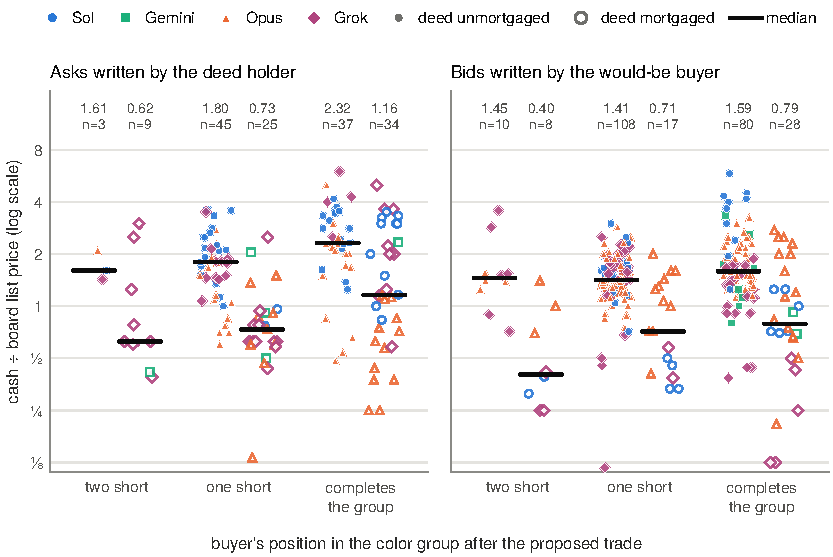
\includegraphics[width=\linewidth]{fig_prices.pdf}
\caption{Cash prices for a single color-group deed, as a multiple of board list price. Each point is one acceptance-legal offer, colored by the system that wrote it. Asks rise as the buyer nears a complete group. Bids rise little. Offers within a thread or game are dependent, and deed mix and game state differ across columns.}
\label{fig:prices}
\end{figure}

Asks rise as the buyer nears a complete group. For unmortgaged deeds the median ask is \fact{d.grad.ask.unmortgaged.2.median} times list when the buyer would still lack two deeds, \fact{d.grad.ask.unmortgaged.1.median} when it would lack one and \fact{d.grad.ask.unmortgaged.0.median} when the deed completes the group. Mortgaged deeds show the same order at lower levels. Bids move much less, with medians of \fact{d.grad.bid.unmortgaged.2.median}, \fact{d.grad.bid.unmortgaged.1.median} and \fact{d.grad.bid.unmortgaged.0.median} for unmortgaged deeds. For a completing, unmortgaged deed the median ask is therefore \fact{d.grad.ask.unmortgaged.0.median} times list and the median bid \fact{d.grad.bid.unmortgaged.0.median}.

The direction of the ask pattern is stable across coarse cuts. Asks to a completing buyer are higher in all \fact{barg.prices.cells-with-at-least-3-each.ask.higher} seller and mortgage-status cells with at least three asks on each side (Appendix~\ref{app:bargaining}), in all \fact{d.ask.stagecells.n} cells formed by thread position and mortgage status, and in \fact{d.ask.blocks.higher} of the 5 seed blocks for unmortgaged deeds. With any one block left out, the median unmortgaged ask stays between \fact{d.ask.lobo.comp.min} and \fact{d.ask.lobo.comp.max} for completing buyers and between \fact{d.ask.lobo.other.min} and \fact{d.ask.lobo.other.max} for others. Bids show no common direction. Sol bids \fact{d.price.bid.Sol.unmortgaged.completes} times list for a deed that completes its own group against \fact{d.price.bid.Sol.unmortgaged.other} otherwise, and Grok bids \fact{d.price.bid.Grok.unmortgaged.completes} against \fact{d.price.bid.Grok.unmortgaged.other}.

The tightest comparison is weaker. In \fact{d.pairs.n} cases one seller prices one deed, within one game, for both a completing and a non-completing buyer. The completing buyer is asked more in \fact{barg.prices.same-game-seller-deed-direction.higher} cases, less in \fact{barg.prices.same-game-seller-deed-direction.lower} and the same in \fact{barg.prices.same-game-seller-deed-direction.equal} (Table~\ref{tab:pairs}). Both of the lower cases are Opus selling Boardwalk as its cash ran down. We therefore report a consistent direction and do not estimate a premium. Counteroffers add a caution. A counter usually keeps the bundle and asks for more cash, and it does so about as often when no one would complete a group (\fact{barg.counters.neither-with-deed-request.same-noncash-bundle-more-cash-to-counterer} of \fact{barg.counters.neither-with-deed-request.counters} counters) as when the original author would (\fact{barg.counters.author-only.same-noncash-bundle-more-cash-to-counterer} of \fact{barg.counters.author-only.counters}). Repricing is how these agents bargain in general. What is specific to completing deeds is the level of the ask and the frequency of outright refusal.

\subsection{What the refusals say}

Two earlier model-assisted readings coded the stated reasons in all \fact{inh.reason.rows} outright rejections of offers that would complete the recipient's own group. Both found a stated consequence for the rival, such as its completion, building funds or survival, in \fact{inh.reason.D.both} (Cohen's $\kappa$ of \fact{inh.reason.D.kappa} between the readings). Both found a stated concern about the recipient's own cash, price or reserves in \fact{inh.reason.C.both} ($\kappa$ of \fact{inh.reason.C.kappa}). The rival code covers \fact{inh.reason.D.both.recipient-only} of the \fact{inh.reason.rows.recipient-only} refusals of offers completing only the recipient's group. By recipient it covers \fact{inh.reason.D.both.Gemini} of \fact{inh.reason.rows.Gemini} for Gemini, \fact{inh.reason.D.both.Grok} of \fact{inh.reason.rows.Grok} for Grok, \fact{inh.reason.D.both.Sol} of \fact{inh.reason.rows.Sol} for Sol and \fact{inh.reason.D.both.Opus} of \fact{inh.reason.rows.Opus} for Opus, whose eight records have no private note. Two games supply \fact{inh.reason.rows.top2games} of the \fact{inh.reason.rows} refusals. The readings came from two instances of one model family, one of them partly exposed to earlier counts, and no human labeled the rows. They establish what the messages and notes say and not why the agents refused. The two incidents below show the content behind the codes.

\IncidentTitle{g2}{A blocker kept while its holder is liquid and has nothing to build (G2)}

At G2 turn 44 Sol holds Marvin Gardens, \$137 and no complete group. Opus holds the other two yellows. Grok owns no yellow and bids \$200.
\TranscriptQuote{g2-d118-liquidity-pitch}
Sol asks \$450 and rejects Grok's \$250. One turn later Opus bids \$325 for the same deed, which would complete its yellows. Sol asks \$650.
\TranscriptQuote{g2-d124-price}
\TranscriptQuote{g2-d124-note}
Sol comes down to \$600 and Opus stops at \$450. Sol's note on its final rejection gives the reason for keeping the deed.
\TranscriptQuote{g2-d128-note}
Twenty-four turns later the positions have reversed. Sol has \$435 and Opus \$17. Sol offers two railroads for Opus's two mortgaged yellows, and Opus replies.
\TranscriptQuote{g2-d197-reverse}
\IncidentOutcome{Sol pays the extra \$100 and completes yellow. Opus is eliminated three turns later owing Gemini \$1,300. Sol builds two houses, sells them four turns after the trade to pay rent, and is eliminated at turn 85. Both estates pass to Gemini, which wins.}
\IncidentReading{Sol prices one deed at \$450 for a buyer with no yellows and \$650 for the buyer it would complete, and its note counts that buyer's remaining building cash. The \$520 figure is right and the house count is wrong, since \$520 buys three yellow houses, and house prices are absent from the prompt at this decision. Both bidders pitch liquidity to a seller holding \$137. Sol declines because it can mortgage other deeds and has no group on which to spend the proceeds. Once Opus is down to \$17, the group changes hands in the other direction.}
\IncidentSource{G2 d118--d128 and d196--d198. Sol and Grok respond under the standard condition. Opus's d197 message is an action-only response. Quoted public messages appear in the named counterparty's next prompt.}

\IncidentTitle{g15}{Refusing one's own complete group three times (G15)}

At G15 turn 63 Sol has \$730 and Grok \$333. One turn earlier Opus had addressed the table.
\TranscriptQuote{g15-d166-appeal}
Sol offers Grok its two greens for Ventnor and \$100. The trade would complete green for Grok and yellow for Sol. Grok refuses, and its note compares what each side could then build.
\TranscriptQuote{g15-d169-refusal-note}
Sol drops its cash request and adds Kentucky. When Grok refuses again, Sol adds \$250 of its own.
\TranscriptQuote{g15-d174-sweetener}
\TranscriptQuote{g15-d175-final-refusal}
Sol's closing note says when it will try again.
\TranscriptQuote{g15-d176-wait-note}
\IncidentOutcome{No trade settles. In the same turn Gemini refuses to sell Sol the deed that would complete light blue. Eighteen turns later Grok is the first player eliminated, and its yellow and green blockers pass to Gemini, which wins. Sol never completes either group.}
\IncidentReading{Grok turns down its own complete group three times because of what the same trade would let Sol build, and Sol reshapes its offer around that objection. Grok's cash arithmetic matches the ledger, though its \$600 is the price of a full first layer on green and one green house costs \$200. The refusals kept two blockers from Sol until Grok's bankruptcy handed them to a third player. Sol's last note states the timing rule that the next section finds in the population.}
\IncidentSource{G15 d166--d176. Opus's appeal is an action-only response and appears in Grok's d169 prompt. All other quoted responses are standard first attempts.}

\section{A blocker moves when its holder is short of cash}
\label{sec:liquidity}

\subsection{Refusal falls with the holder's cash}

Figure~\ref{fig:liquidity}a splits the \fact{barg.census.cells.author-only.n} completion requests by the holder's cash when the request arrives. Holders with under \$100 reject \fact{d.holder.lt100.rejectpct}\% of them. Holders with \$100 to \$299 reject \fact{d.holder.100-299.rejectpct}\%, and the two richer groups reject \fact{d.holder.300-599.rejectpct}\% and \fact{d.holder.600plus.rejectpct}\%. Counters make up most of the difference. Acceptance on the spot stays rare at every level, at \fact{d.holder.lt100.acceptpct}\% for the poorest holders and \fact{d.holder.600plus.acceptpct}\% for the richest.

\begin{figure}[t]
\centering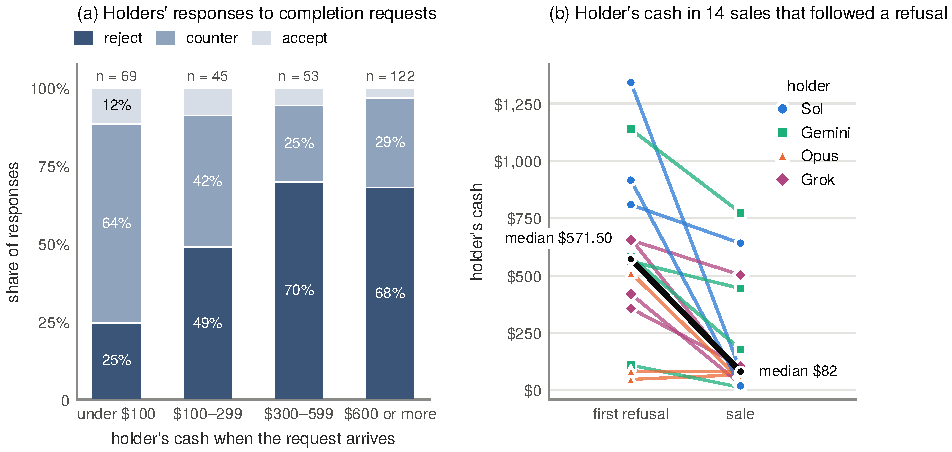
\includegraphics[width=\linewidth]{fig_liquidity.pdf}
\caption{Liquidity and release. (a)~Responses to completion requests by the holder's cash. (b)~Holder's cash when it first rejected or countered the buyer's request and when it later sold, for the one-sided sales with such an earlier refusal. Each line is one holder, buyer and color group. The black line joins the medians.}
\label{fig:liquidity}
\end{figure}

The contrast between holders under \$100 and holders with \$300 or more is \fact{d.gap.low.pct}\% against \fact{d.gap.high.pct}\%. It has the same sign in each of the five seed blocks and in \fact{barg.holder-cash.reject-gap-games-with-both-strata.0} of the \fact{barg.holder-cash.reject-gap-games-with-both-strata.1} games that contain both kinds of request. With any one block removed it ranges from \fact{d.gap.lobo.min} to \fact{d.gap.lobo.max} percentage points.

The contrast shrinks under composition checks and does not vanish. Within opening offers the two shares are \fact{d.gap.opening-only.low.pct}\% and \fact{d.gap.opening-only.high.pct}\%, and within later offers \fact{d.gap.later-only.low.pct}\% and \fact{d.gap.later-only.high.pct}\%. Without Opus as holder they are \fact{d.gap.excluding-opus-recipients.low.pct}\% and \fact{d.gap.excluding-opus-recipients.high.pct}\%, and without Opus on either side \fact{d.gap.excluding-opus-either-side.low.pct}\% and \fact{d.gap.excluding-opus-either-side.high.pct}\%. Without the offers that follow a conflicting Grok call they are \fact{d.grok.excl.gap.low.pct}\% and \fact{d.grok.excl.gap.high.pct}\%. Sol and Grok show the pattern individually. Sol rejects \fact{d.holder.Sol.lt100.rejectpct}\% of requests when it holds under \$100 and \fact{d.holder.Sol.300plus.rejectpct}\% when it holds \$300 or more, and Grok \fact{d.holder.Grok.lt100.rejectpct}\% and \fact{d.holder.Grok.300plus.rejectpct}\%. Gemini is the exception. It rejects \fact{barg.holder-cash.author-only-by-recipient-and-cash.Gemini.lt100.reject} of \fact{barg.holder-cash.author-only-by-recipient-and-cash.Gemini.lt100.n} requests even when it holds under \$100. Opus rejects almost nothing at any level.

Low cash also softens refusals of deeds that complete nothing, where the shares are \fact{d.gap.other-deed-requests.low.pct}\% and \fact{d.gap.other-deed-requests.high.pct}\%. Part of the association is therefore a general effect of needing money. Buyers also send completion requests where cash is short. A holder with under \$100 receives \fact{d.target.completion.pct}\% of them, against \fact{d.target.other.pct}\% of requests for deeds that complete nothing.

\subsection{Following each pair over time}

An offer is a poor unit for a claim about release, because one stubborn pair can produce twenty of them. We therefore group offers into pairs. A pair is a game, a would-be completer, a holder and a color group, with at least one legal offer, written by either party, under which the completer would obtain the group from the holder. The cohort has \fact{barg.dyads.dyads} pairs. A trade settles \fact{barg.dyads.settled} of them, which are the \fact{groups.routes.trade} groups completed by trade. In \fact{barg.dyads.settled-one-sided} the sale completes a group for the buyer only, and we call these one-sided sales. In \fact{barg.dyads.settled-mutual} a swap completes a group for both parties.

One-sided sales come disproportionately from holders short of cash. In \fact{barg.dyads.one-sided-holder-cash-at-settlement.lt100} of the \fact{barg.dyads.settled-one-sided} the holder has under \$100 at settlement, and the median is \$\fact{barg.dyads.one-sided-holder-cash-median}. In the \fact{barg.dyads.settled-mutual} swap completions the median is \$\fact{d.pairs.mutual.median}, and \fact{barg.dyads.mutual-holder-cash-at-settlement.lt100} holder has under \$100.

The sharper evidence follows a pair through time. In \fact{barg.dyads.from-first-holder-decline.n} one-sided sales the holder had rejected or countered a request from the same buyer on an earlier turn. Figure~\ref{fig:liquidity}b shows the holder's cash at that first refusal and at the sale, a median of \fact{d.pairs.decline.medianturns} turns later. It is lower at the sale in \fact{barg.dyads.from-first-holder-decline.lower} of the \fact{barg.dyads.from-first-holder-decline.n} pairs and higher in \fact{barg.dyads.from-first-holder-decline.higher}, and the median falls from \$\fact{d.pairs.decline.median.first} to \$\fact{d.pairs.decline.median.sale}. The comparison holds the holder, the buyer and the group fixed. All four systems appear as holders, and with Opus's \fact{barg.dyads.from-first-holder-decline.by-holder-model.Opus} pairs removed the count is \fact{barg.dyads.from-first-holder-decline.lower-excluding-opus-holders.0} of \fact{barg.dyads.from-first-holder-decline.lower-excluding-opus-holders.1}. The pairs come from \fact{d.pairs.decline.games} games in \fact{d.pairs.decline.blocks} of the five seed blocks (Table~\ref{tab:dyads}). Four more one-sided sales settled on a later turn after the buyer, not the holder, had turned down earlier terms. Counting all \fact{barg.dyads.within-dyad-one-sided-later-turn.n} from the pair's first offer, the holder's cash is lower at the sale in \fact{barg.dyads.within-dyad-one-sided-later-turn.lower}. In the \fact{barg.dyads.unsettled-multi-turn.n} pairs that drew offers on more than one turn and never settled, the holder's cash moved much less, from a median of \$\fact{d.pairs.unsettled.median.first} at the first offer to \$\fact{d.pairs.unsettled.median.last} at the last.

This is not a controlled contrast. Turns pass between the two moments, the board changes, and holders who ran short may differ from those who did not. It is the pattern expected if a blocker is a reserve that its holder gives up when cash runs out, and the agents describe it that way. Sol's notes say it will revisit monopoly trades when opponents need cash (Incident~\ref{inc:g15}) and that it would \InlineQuote{in-g1-d313-distress} (G1 d313).

\subsection{Short of cash is not the same as cheap}

Among one-sided sales for cash alone, the \fact{d.settle.under-100-opus.n} made by Opus with under \$100 settled at a median of \fact{d.settle.under-100-opus} times list price. The \fact{d.settle.under-100-other.n} made by the other systems with under \$100 settled at a median of \fact{d.settle.under-100-other} times list. Of Opus's sales, \fact{d.settle.low.opus.below} were below list price, and of the others' sales \fact{d.settle.low.other.above} were above it. Opus made \fact{barg.dyads.one-sided-under-100-by-holder-model.Opus} of the \fact{barg.dyads.one-sided-holder-cash-at-settlement.lt100} low-cash one-sided sales, nearly all under action-only recovery. As a holder it settled \fact{barg.dyads.settled-by-holder-model.Opus.0} of its \fact{barg.dyads.settled-by-holder-model.Opus.1} pairs, against \fact{barg.dyads.settled-by-holder-model.Sol.0} of \fact{barg.dyads.settled-by-holder-model.Sol.1} for Sol, \fact{barg.dyads.settled-by-holder-model.Gemini.0} of \fact{barg.dyads.settled-by-holder-model.Gemini.1} for Gemini and \fact{barg.dyads.settled-by-holder-model.Grok.0} of \fact{barg.dyads.settled-by-holder-model.Grok.1} for Grok. The cohort cannot say how much of this belongs to the model and how much to its response condition. It does show that cash pressure and a low price are separable. The other three systems released deeds when short of cash and still charged for the buyer's monopoly.

\IncidentTitle{g1}{A completing deed sold for a quarter of its list price (G1)}

Opus holds Boardwalk and Grok holds Park Place. From G1 turn 69, when it has \$453, Opus offers Boardwalk seven times in exchange for New York Avenue, a swap that would complete orange for Opus as well as dark blue for Grok. Grok rejects six of the offers and counters one. At turn 122 Opus pays a \$550 rent by mortgaging a railroad, which leaves it \$18, and offers the mortgaged deed for cash alone.
\TranscriptQuote{g1-d306-offer}
\TranscriptQuote{g1-d307-counter}
Opus asks \$100 and adds that \InlineQuote{in-g1-d308-weapon}. Grok accepts above its own ceiling.
\TranscriptQuote{g1-d309-accept-note}
\IncidentOutcome{Grok completes dark blue for \$100, a quarter of Boardwalk's list price. It never redeems the mortgage or builds. Over the next 94 turns opponents land on the group five times and pay \$70 in total. Opus is eliminated four turns after the sale, owing Gemini \$550. Gemini wins.}
\IncidentReading{Between its first offer and the sale the holder's cash fell from \$453 to \$18, and its terms fell from a deed that would complete its own group to \$100. Opus presents the sale as arming a rival of the leader. Grok's note prices the alternative, in which Opus goes bankrupt and Boardwalk passes to the leader with the estate. Opus's side has no private note, because it played under action-only recovery.}
\IncidentSource{G1 d305--d315. Grok's responses are standard first attempts. Opus's are action-only responses. The quoted public messages appear in the counterparty's next prompt.}

\IncidentTitle{g13}{Distress used as a bargaining position (G13)}

At G13 turn 107 Grok has \$35, owns the three yellows and stands nine squares before Short Line, where Sol's four railroads charge \$200. Its Ventnor Avenue is unmortgaged and would raise \$130. Grok offers Opus its mortgaged Pennsylvania Avenue for \$200.
\TranscriptQuote{g13-d250-insurance}
Opus counters at \$130. Grok holds at \$200 and tells Opus that \$130 would leave it \$35 short. Its private note and the explanation returned with the same response say more.
\TranscriptQuote{g13-d252-floor}
\TranscriptQuote{g13-d252-omission}
\TranscriptQuote{g13-d253-accept}
\IncidentOutcome{Opus pays \$200 and \$16 of mortgage-transfer interest. Seven turns later it buys North Carolina at auction for \$650 and completes green. Grok's next roll misses Short Line. It pays \$200 on another of Sol's railroads at turn 146 and goes bankrupt on Short Line at turn 150, and the yellows pass to Sol. Opus wins.}
\IncidentReading{Grok presents its own distress as the buyer's problem, since Sol would inherit the yellows if Grok failed. It asks \$200 while its note sets a floor of \$165, and the returned explanation records that it left out the Ventnor mortgage. Under this prompt that is an authorized public bluff. Opus pays the asking price, and nothing in the record shows that it believed the claimed limit or that the omission produced the extra \$70. The pitch also overstates the risk. Short Line is nine squares away, a 4-in-36 chance on one roll, as Grok's own note says.}
\IncidentSource{G13 d250--d253. Grok's responses are standard first attempts. Opus's are action-only responses. The returned explanation is the provider's reasoning field, a channel separate from the private note.}

\section{What the cash becomes separates the trajectories}
\label{sec:conversion}

\subsection{Sellers: paying for houses or postponing insolvency}

A sale that completes a rival's group can serve two purposes. It can raise cash to survive, or it can pay for houses on the seller's own group. We split the \fact{barg.dyads.settled-one-sided} one-sided sales by whether the seller bought at least one house or hotel within eight turns of the sale, which is two rounds of a full table (Table~\ref{tab:sellers}).

\begin{table}[t]
\centering\small
\begin{tabular}{@{}llrrrr@{}}
\toprule
& & & Seller & Seller later & Median turns\\
Seller's cash at the sale & After the sale the seller & Sales & won & eliminated & to elimination\\
\midrule
\SellerRows
\bottomrule
\end{tabular}
\caption{What followed the \fact{barg.dyads.settled-one-sided} sales that completed a color group for the buyer only. A seller can build only on a complete group of its own, so the split also reflects the seller's position at the time of the sale.}
\label{tab:sellers}
\end{table}

In \fact{conv.seller-conversion.all-one-sided.built-after-sale.n} sales the seller built, and \fact{conv.seller-conversion.all-one-sided.built-after-sale.seller-won} of those sellers won the game. In \fact{conv.seller-conversion.all-one-sided.no-construction-after-sale.n} the seller did not build, and \fact{conv.seller-conversion.all-one-sided.no-construction-after-sale.seller-won} won. The split is sharpest among sellers with under \$100. Of these, \fact{conv.seller-conversion.seller-under-100.built-after-sale.n} built and \fact{conv.seller-conversion.seller-under-100.built-after-sale.seller-won} of them won. The other \fact{conv.seller-conversion.seller-under-100.no-construction-after-sale.n} did not build. All of them were eliminated, a median of \fact{conv.seller-conversion.seller-under-100.no-construction-after-sale.median-turns-to-elimination} turns after the sale, and none won. Windows of four and twelve turns give the same picture (Appendix~\ref{app:development}).

Sales are not independent, since one player can sell twice. The \fact{conv.seller-conversion.all-one-sided.built-after-sale.n} sales followed by building were made in \fact{conv.seller-conversion.all-one-sided.built-after-sale.distinct-seller-player-games} player-games, \fact{conv.seller-conversion.all-one-sided.built-after-sale.distinct-winning-seller-player-games} of which ended in a win. The other \fact{conv.seller-conversion.all-one-sided.no-construction-after-sale.n} were made in \fact{conv.seller-conversion.all-one-sided.no-construction-after-sale.distinct-seller-player-games} player-games, \fact{conv.seller-conversion.all-one-sided.no-construction-after-sale.distinct-winning-seller-player-games} of which ended in a win. In \fact{conv.seller-conversion.all-one-sided.built-after-sale.distinct-winning-seller-player-games} of the 20 games, then, the eventual winner sold a rival its completing deed and built within eight turns. Winners in this cohort did sell rivals their completing deeds. They sold when they had a group of their own to build on, and they put the money there. This is a description and not a causal estimate, since building after a sale marks a stronger position as well as a use of funds.

\IncidentTitle{g7}{A bid timed to the holder's cash, and a sale that pays for houses (G7)}

At G7 turn 25 Sol holds \$1,150 and has just bought North Carolina for \$300. Grok bids \$500 for it, which would give Grok two of the three greens.
\TranscriptQuote{g7-d39-liquid}
Grok bargains the price down with a public limit that its private note does not hold.
\TranscriptQuote{g7-d42-final}
\TranscriptQuote{g7-d42-ceiling}
Sol accepts \$600 and notes that it will \InlineQuote{in-g7-d43-reinvest}. Forty-two turns later Sol buys Park Place from Opus for \$800 and a deed, builds three houses on the dark blues and is left with \$84. Gemini needs Sol's New York Avenue to complete orange. It had bid \$350 for that deed fifteen turns earlier, when Sol held \$1,342, and no sale followed. It bids \$350 again now.
\TranscriptQuote{g7-d141-timed-bid}
Sol asks \$700.
\TranscriptQuote{g7-d142-ask-note}
\IncidentOutcome{Gemini pays \$700, mortgages five deeds and builds four orange houses in the same turn. Sol buys three more dark-blue houses within eight turns. Gemini's oranges collect \$270 before Gemini is eliminated at turn 125 owing Sol \$1,400. Sol wins.}
\IncidentReading{Holding \$1,150, Sol calls itself liquid and charges twice list price for a deed that completes nothing. Holding \$84 and a group to build on, it sells the deed that completes a rival's group at three and a half times list, and its note sets that price by what the money lets Sol build and what it leaves the buyer. Gemini's note shows a buyer timing its bid to the holder's low cash. Grok's ``final'' price is an authorized bluff that happened to settle, and nothing in the record shows that it moved the price.}
\IncidentSource{G7 d39--d43 and d132--d150. All quoted responses are standard first attempts. The quoted public messages appear in the counterparty's next prompt.}

\subsection{Buyers: completing a group and building on it}

The same question applies to the buyer. Table~\ref{tab:conversion} follows all \fact{groups.routes.trade} groups completed by trade from completion until their owner lost them or the game ended.

\begin{table}[!htb]
\centering\small
\begin{tabular}{@{}lrrrr@{}}
\toprule
& Sol & Gemini & Opus & Grok\\
\midrule
\ConversionRows
\bottomrule
\end{tabular}
\caption{The \fact{groups.routes.trade} color groups completed by trade. A landing is an opponent's move that ends on a deed of the group while the owner holds it. Rent is the amount paid on those landings. $^{\dagger}$The first-management-turn row uses a classification inherited from earlier work. All other rows are fresh tabulations from events. Opus's column describes play mostly under action-only recovery.}
\label{tab:conversion}
\end{table}

The four systems complete similar numbers of groups. Sol builds in its first management turn after completion on \fact{inh.window.Sol.built} of \fact{inh.window.Sol.groups} and Gemini on \fact{inh.window.Gemini.built} of \fact{inh.window.Gemini.groups}. Opus does so on \fact{inh.window.Opus.built} of \fact{inh.window.Opus.groups} and Grok on \fact{inh.window.Grok.built} of \fact{inh.window.Grok.groups}.

\begin{figure}[!htb]
\centering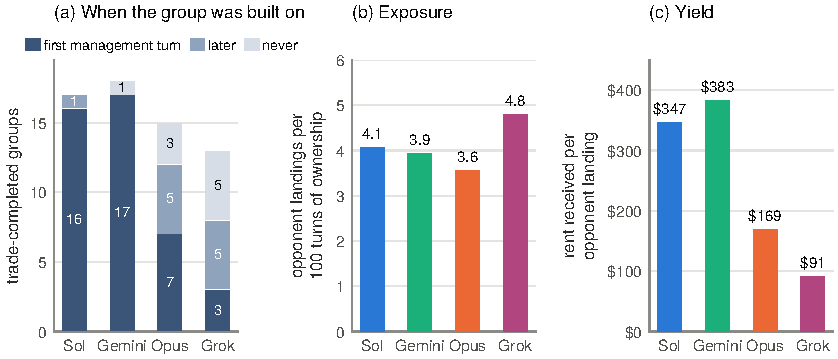
\includegraphics[width=\linewidth]{fig_conversion.pdf}
\caption{What followed a completion by trade. (a)~When the owner first built on the group. (b)~How often opponents landed on it. (c)~How much rent each landing paid. Exposure is similar across systems and the rent per landing is not.}
\label{fig:conversion}
\end{figure}

The difference in rent does not come from exposure (Figure~\ref{fig:conversion}). Opponents landed on these groups at similar rates, between \fact{d.conv.landrate.min} and \fact{d.conv.landrate.max} times per 100 turns of ownership, and Grok's groups were landed on most often. Groups built in the first management turn and groups not built then were held for similar lengths of time, with median durations of \fact{conv.trade-groups.first-window-built.median-duration} and \fact{conv.trade-groups.first-window-not-built.median-duration} turns and landing rates of \fact{d.conv.early.landrate} and \fact{d.conv.late.landrate} per 100 turns. What differs is the rent charged at each landing. Sol and Gemini received \$\fact{d.conv.rpl.Sol} and \$\fact{d.conv.rpl.Gemini} per opponent landing, Opus \$\fact{d.conv.rpl.Opus} and Grok \$\fact{d.conv.rpl.Grok}. Sol and Gemini together exceed Opus and Grok together in each of the \fact{d.conv.blocks.ordered} seed blocks. The \fact{conv.trade-groups.first-window-built.groups} groups built at once collected \$\fact{conv.trade-groups.first-window-built.rent} of the \$\fact{conv.trade-groups.total-rent} paid on all \fact{groups.routes.trade}, or \$\fact{d.conv.early.rentperlanding} per landing against \$\fact{d.conv.late.rentperlanding}. Landings are few. Five groups account for \fact{d.conv.top5.pct}\% of the rent, so the dollar totals rest on a small number of dice outcomes. Figure~\ref{fig:timeline} in the appendix draws every group.

An earlier classification, which we inherit, says why \fact{d.conv.unbuilt.n} groups went unbuilt in the first management turn. In \fact{conv.trade-groups.inherited-first-window-causes.never-legal-in-window} no build on the group was legal during that turn, and \fact{d.conv.noopt.mortgaged} of those groups held a mortgaged deed at completion. In \fact{d.conv.defaults} the engine applied a default after an invalid build request, in \fact{conv.trade-groups.inherited-first-window-causes.received-conflict} Grok's applied call ended the turn while its text requested a build, and in \fact{conv.trade-groups.inherited-first-window-causes.valid-end} the owner validly ended the turn. Opus's \fact{d.conv.unbuilt.n.Opus} unbuilt groups are \fact{inh.window.Opus.never-legal-in-window} windows with no legal build and \fact{inh.window.Opus.default-after-refusal} defaults. Part of its gap is therefore its response condition, since an invalid action-only build plan gets no correction, and part is the state in which it bought. It completed \fact{conv.trade-groups.by-model.Opus.mortgaged-deed-at-completion} of its \fact{conv.trade-groups.by-model.Opus.groups} groups with a mortgaged deed in them and held a median of \$\fact{conv.trade-groups.by-model.Opus.median-cash-after-completion} afterwards. Grok's \fact{d.conv.unbuilt.n.Grok} are \fact{inh.window.Grok.never-legal-in-window} windows with no legal build, in which its notes defer redemption to keep cash, \fact{inh.window.Grok.received-conflict} conflicting calls and \fact{inh.window.Grok.valid-end} stated holds. Grok held a median of \$\fact{conv.trade-groups.by-model.Grok.median-cash-after-completion} after its trades, enough for a house in most groups.

\IncidentTitle{g20}{Rivals try to stop a sale from becoming houses (G20)}

At G20 turn 22 Opus sells Illinois to Grok for \$500. The sale completes Grok's reds and leaves it \$222, and a red house costs \$150. Two turns later Sol's private note says \InlineQuote{in-g20-d95-cashstarved}. Gemini then says the same in public.
\TranscriptQuote{g20-d96-appeal}
Grok's next note registers the appeal.
\TranscriptQuote{g20-d97-recognition}
On its next turn Grok builds one house on each red, which leaves it \$7, and mortgages New York Avenue. It then tries to sell Vermont to Gemini.
\TranscriptQuote{g20-d100-sale}
\TranscriptQuote{g20-d101-refusal}
\IncidentOutcome{Grok mortgages Vermont for \$50. Opus later bids for two of Grok's mortgaged deeds, telling it \InlineQuote{in-g20-d129-houses}, and Grok holds out for more than Opus will pay. Opponents land on Grok's reds twice and pay \$126. Grok is the first player eliminated, at turn 84. Gemini wins.}
\IncidentReading{Gemini and Sol both treat cash paid to Grok as houses on the reds, which is the conversion this section describes, seen by the players it threatens. Gemini asks the table to withhold the cash and then refuses a purchase itself. Opus does the opposite and offers Grok money for houses. The appeal is one player's request and its own follow-through. It is not a cartel.}
\IncidentSource{G20 d95--d102, d129--d130 and d156--d160. Grok's quoted note belongs to the selected second attempt at d97, after a malformed first attempt. Opus's later bids are action-only responses.}

\section{Forced finance is reliable, and default redistributes the board}
\label{sec:default}

\subsection{All debt episodes}

A player whose debt exceeds its cash must raise money from a menu of mortgages and building sales, or declare bankruptcy. The cohort has \fact{debt.episodes} such debt episodes, \fact{debt.reasons.RENT} of them for rent. Players paid \fact{debt.paid} and were eliminated in \fact{debt.eliminated} (Figure~\ref{fig:debt}).

\begin{figure}[!htb]
\centering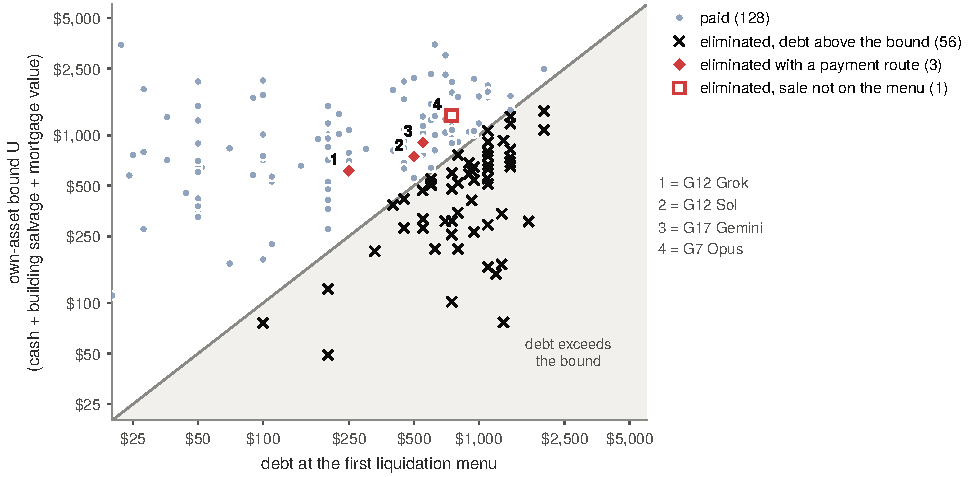
\includegraphics[width=0.92\linewidth]{fig_debt.pdf}
\caption{All \fact{debt.episodes} debt episodes at their first liquidation menu. The bound $U$ adds cash, the salvage value of every building and the mortgage value of every unmortgaged deed. A debt above $U$ cannot be paid from the player's own assets. Payment routes for the three numbered diamonds and the menu restriction for the square are inherited from earlier engine-executed checks.}
\label{fig:debt}
\end{figure}

For each episode we compute an own-asset bound $U$ at the first menu. It is the player's cash plus the salvage value of all its buildings plus the mortgage value of all its unmortgaged deeds. The bound ignores sale-order and bank-stock restrictions, so a debt above $U$ cannot be paid from the player's own assets. That is the case in \fact{debt.classes.below-bound} eliminations. For the other four we inherit earlier results. Legal payment sequences exist for three. The fourth, Opus in G7, could not pay. With no houses left in the bank, its menu offered no building sale on a group that carried a hotel and eight houses.

So \fact{debt.feasible-episodes} episodes had a payment route, and players took it in \fact{debt.paid}, or \fact{d.debt.paid.pct}\%. Each system paid nearly every payable debt. Sol paid \fact{debt.by-model.Sol.paid} of \fact{d.debt.Sol.payable}, Gemini \fact{debt.by-model.Gemini.paid} of \fact{d.debt.Gemini.payable}, Opus \fact{debt.by-model.Opus.paid} of \fact{d.debt.Opus.payable} and Grok \fact{debt.by-model.Grok.paid} of \fact{d.debt.Grok.payable}. Opus did so under action-only recovery and without notes. Many payments were close. In \fact{debt.paid-bound-minus-debt.under-250} of the \fact{debt.paid} the bound exceeded the debt by less than \$250. In G20 Sol met a \$\fact{d.debt.g20.debt} rent in \fact{d.debt.g20.actions} consecutive actions that sold every building on two groups and mortgaged \fact{d.debt.g20.mortgages} deeds, and it finished with \$\fact{d.debt.g20.left}. Of the \fact{debt.paid-with-sale} payments that sold buildings, only \fact{debt.paid-sale-when-menu-mortgages-cover-shortfall} did so when the mortgages on the first menu would have covered the shortfall.

The three payable eliminations are two miscalculations and one conflict. In their notes, Sol in G12 and Gemini in G17 each add up cash, building salvage and the mortgages currently on the menu, and leave out the mortgages that selling the buildings would unlock. The third is Incident~\ref{inc:g12}. Unlike the decisions in Sections~\ref{sec:liquidity} and~\ref{sec:conversion}, paying a debt comes with an explicit menu, a stated amount and an immediate test of success, and all four systems do it well.

\IncidentTitle{g12}{A payable debt ends in bankruptcy through conflicting channels (G12)}

At G12 turn 101 Grok owes Opus \$250 and has \$43. Its pink group carries two, two and three houses, and the menu offers a sale on Virginia Avenue. The text of Grok's response requests that sale.
\TranscriptQuote{g12-d249-content}
The private note attached to the same response works through the arithmetic and ends as follows.
\TranscriptQuote{g12-d249-note}
The one tool call in the response declares bankruptcy, with this public message.
\TranscriptQuote{g12-d249-public}
\IncidentOutcome{The engine applies the call. Grok is eliminated without selling a house, and its estate passes to Opus, which wins. An earlier engine-executed check, which we inherit, found five legal house sales from this state that pay the debt and leave \$43. The two-house sale named in the text is legal and would have raised Grok's cash to \$143, short of the debt.}
\IncidentReading{The note first calls payment impossible, then finds the five-sale route and its correct remainder, and the applied action contradicts it. The case separates finding a payment route from executing one. It is an instance of the Grok condition in Section~\ref{sec:conditions}, and the record cannot say which channel shows what the system would have done.}
\IncidentSource{G12 d249, a standard first attempt. The text channel is the assistant content of the response and was not applied.}

\subsection{Estates and the positions they reach}

A player-creditor receives the eliminated player's estate. Forty eliminations precede the last one of their game. The eventual winner is the creditor in \fact{flows.creditor-is-winner-nonterminal} of them and receives \fact{flows.estate-deeds-nonterminal-to-winner} of the \fact{flows.estate-deeds-nonterminal} deeds they transfer. The first estate goes to the eventual winner in \fact{estate.first-creditor-is-winner} of 20 games. In \fact{flows.developed-rent-debts-all} of the 60 eliminations the debt is rent on a creditor's developed deed.

These counts could mean only that the leader collects. Figure~\ref{fig:estates} tests that reading by placing every player just before the first elimination, with assets valued as cash, plus deeds at list price or half of it if mortgaged, plus buildings at cost. The first creditor held the largest share in \fact{estate.first-creditor-leads-assets} games and owned a developed group in all \fact{estate.creditor-has-developed-group}. In most games, then, the first estate went to the player already ahead.

\begin{figure}[!htb]
\centering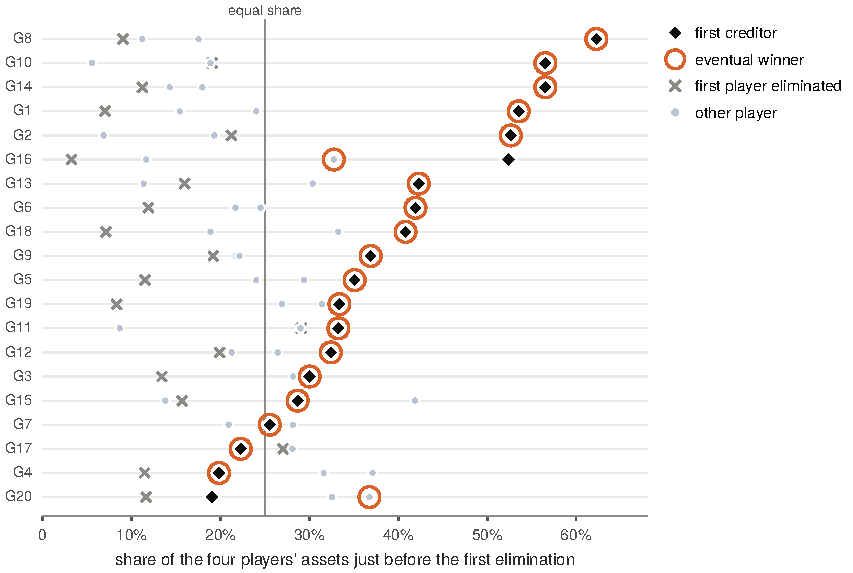
\includegraphics[width=0.86\linewidth]{fig_estates.pdf}
\caption{Each player's share of total assets at the first liquidation menu of the debt that ends in the game's first elimination. Assets are cash, deeds at list price (half if mortgaged) and buildings at cost. Games are ordered by the first creditor's share.}
\label{fig:estates}
\end{figure}

The other \fact{d.estate.discordant} games carry the information. In G4, G7, G15 and G17 the first creditor did not lead in assets and went on to win. In G20 it did not lead and lost. Where the creditor already led, it won \fact{d.estate.leader.creditorwins} of \fact{estate.first-creditor-leads-assets} games. G17 is the clearest case. Gemini declared bankruptcy on a \$550 rent with a payment route available, after telling the table that it was short.
\TranscriptQuote{g17-d234-public}
Its estate held six deeds, among them Park Place and Boardwalk with five houses. It went to Sol, which had the smallest asset share at the table and \$34 in cash, and Sol won. Five games cannot show that estates decide winners. They show that the first estate is more than a marker of who was already ahead.

Estates also end most of the stand-offs that bargaining does not. Of the \fact{barg.dyads.unsettled} pairs that never settled, the group was next completed through an estate in \fact{barg.dyads.unsettled-resolved-by-estate}, and \fact{barg.dyads.unsettled-resolved-by-nonterminal-estate} of those came before the game's last elimination. In \fact{barg.dyads.unsettled-same-completer-via-estate} the same would-be buyer received the group that way and paid nothing. A holder's refusal lasts only as long as the holder does. The agents in Incidents~\ref{inc:g1} and~\ref{inc:g13} bargain over exactly that, and the buyer in the last incident acts on it.

\IncidentTitle{g18}{A buyer stops buying once the seller needs the money (G18)}

At G18 turn 181 Opus holds \$615 and bids \$200 and then \$250 for Sol's mortgaged Pacific, which would complete Opus's greens. Sol holds \$294 and asks \$600.
\TranscriptQuote{g18-d420-note}
Sol rejects \$250. Over the next six turns Opus says four times that the offer still stands, the last time after collecting a \$750 rent from Sol.
\TranscriptQuote{g18-d431-assurance}
A second \$750 rent then forces Sol to sell its orange hotels and mortgage its reds, which leaves it \$49. Sol offers Pacific in a bundle for \$450 and then \$350 to pay for new orange houses, and Opus passes on both. Sol then names the price Opus had advertised.
\TranscriptQuote{g18-d441-invocation}
\TranscriptQuote{g18-d442-withdrawal}
\TranscriptQuote{g18-d442-explanation}
\IncidentOutcome{No sale occurs. Sol's note reads \InlineQuote{in-g18-d443-rebuild}. Opus, holding \$2,125, redeems its two green deeds over the next four turns and bids \$150 and \$225 for Pacific. Sol asks \$450, \$350 and \$300, and nothing settles. Sol is eliminated at turn 197, its estate passes to Opus, and Opus wins.}
\IncidentReading{While Sol had cash it priced the blocker at \$600. Down to \$49, it offered the same deed at the buyer's own price so that it could rebuild, and the buyer declined. Opus's returned explanation says that buying would only extend a nearly bankrupt rival's life, and as Sol's likely creditor it could expect the deed anyway. The assurance was a public message that the engine does not enforce, and nothing shows that it was insincere when made.}
\IncidentSource{G18 d419--d461. Sol's responses are standard first attempts. Opus's are action-only responses, and the explanation is the provider's reasoning field.}

\section{Discussion}
\label{sec:discussion}

\subsection{Attention is common and conversion is not}

The evidence sits at three levels. On attention the result is strong and shared by all four systems. They refuse, reprice or publicly contest trades by reference to what the trade gives a rival, and their notes say so. On pricing the result is directional. Asks to completing buyers are higher in every coarse cut, but the matched cases are mixed, bids show no common direction, and the stated arithmetic is sometimes wrong. On outcomes, attention is not what separates the systems. Grok refuses \fact{d.holder.Grok.300plus.rejectpct}\% of completion requests while it is liquid and states a rival consequence in \fact{inh.reason.D.both.Grok} of its \fact{inh.reason.rows.Grok} refusals of its own completion, yet it built at once on \fact{inh.window.Grok.built} of \fact{inh.window.Grok.groups} groups and collected \$\fact{d.conv.rpl.Grok} per opponent landing. Sol counters where Grok refuses, sells a blocker when it has something to build, and built at once on \fact{inh.window.Sol.built} of \fact{inh.window.Sol.groups}. Gemini refuses as often as Grok and builds like Sol. On question A, then, this cohort points one way. Speaking and acting on a rival-aware view is common to these systems. Turning a position into income is rarer, and it is where their trajectories differ.

None of this shows that building caused winning. Opus's building gap is partly its response condition, and Grok's is partly its conflicting calls. Wins of \fact{d.wins.Sol}, \fact{d.wins.Gemini}, \fact{d.wins.Opus} and \fact{d.wins.Grok} by system sit beside wins of \fact{conv.cohort.wins-by-seat.1}, \fact{conv.cohort.wins-by-seat.2}, \fact{conv.cohort.wins-by-seat.3} and \fact{conv.cohort.wins-by-seat.4} by seat, and twenty games cannot tell skill from seat and dice.

\subsection{Two results from bargaining theory}

The observations fit two established results. Jehiel and Moldovanu show that negative externalities among potential buyers can delay a sale under complete information, because what a party will pay depends on who would otherwise obtain the object~\cite{jehiel1995delay}. Our holders are in a stronger version of that position, since the seller itself will pay rent to the buyer. They also tie their result to Rubinstein's point that the cost of rejecting an offer determines the outcome~\cite{rubinstein1982perfect}, and a holder short of cash has a high cost of waiting. Shleifer and Vishny show that a distressed seller receives less than an asset's value in best use when its natural buyers are constrained~\cite{shleifer1992liquidation,shleifer2011firesales}. Here the natural buyer of a completing deed is a single rival. Even so, three of the four systems mostly sold above list price when short of cash, and the low prices came from Opus. We test neither theory. They suggest that this behavior is what bargaining under externalities and cash constraints tends to produce, and that it is not peculiar to these systems.

\subsection{What would count against this account}

Each claim has an observation that would contradict it. The liquidity account fails if, in a new cohort, liquid holders release completing deeds as readily as cash-poor ones, or if holders who sell after refusing have not lost cash in between. The pricing claim reduces to composition if asks stop rising with the buyer's proximity once deed and state are matched in adequate numbers. With seven matched cases, that claim is the weakest here. The conversion contrast is a cohort accident if sellers who build after selling win no more often than those who do not. The reliability of forced finance fails if payable debts go unpaid at a material rate under the same menu.

\subsection{The motivating questions}

Table~\ref{tab:questions} states what this cohort shows about each of the eight questions and A to C, and what it does not measure. An unmeasured construct is not a negative finding about capability.

\begingroup\footnotesize
\renewcommand{\arraystretch}{1.12}
\begin{longtable}{@{}L{0.20\linewidth}L{0.45\linewidth}L{0.29\linewidth}@{}}
\caption{Coverage of the motivating questions. ``Inherited'' marks results from earlier work that this paper did not rerun.}\label{tab:questions}\\
\toprule
Question & What this cohort shows & Not measured\\
\midrule\endfirsthead
\toprule
Question & What this cohort shows & Not measured\\
\midrule\endhead
\bottomrule\endfoot
1. Strategic reasoning & Agents routinely reject trades that would help them because of what a rival gains. They reject \fact{barg.census.cells.recipient-only.reject} of \fact{barg.census.cells.recipient-only.n} offers completing only their own group and state a rival consequence in \fact{inh.reason.D.both} of \fact{inh.reason.rows} such refusals (inherited readings). & Whether any refusal was correct. Regret and exploitability.\\
2. Opponent modeling & Agents track rivals' public cash and building capacity, send completion requests to holders short of cash (\fact{d.target.completion.pct}\% against \fact{d.target.other.pct}\% for other requests) and name who would inherit an estate. & Accuracy or calibration of beliefs about hidden intentions.\\
3. Negotiation, cooperation and deception & A full response census. Counters reprice the same bundle. Incidents show authorized bluffs, selective disclosure, a withdrawn assurance and two public appeals to deny a rival deeds or funds. Acceptance is \fact{barg.census.responses-all.accept} of \fact{barg.census.responses-all.n} responses, so no general bias toward agreement appears. & Persuasion effects, joint surplus, fairness and the prevalence of deception.\\
4. Planning and memory & Stated timing rules that match later population behavior (Sol waits for opponents to need cash). Systems differ in whether cash is held or built with. One multi-turn building target was reached in G9 (inherited). & Benefit of memory and plan-completion rates. Opus mostly lacked its own notes.\\
5. Adaptation and learning & Holders change terms as their cash changes. After a corrective message, 9 of 50 later build submissions repeated an uneven-build error, against 54 of 59 without one, all of the latter Opus (inherited). & Learning caused by feedback. Adaptation to unfamiliar opponents.\\
6. Economic decisions and risk & Prices relative to list by role and position. \fact{debt.paid} of \fact{debt.feasible-episodes} payable debts paid. Rent per landing and construction after sales by system. & Whether any price or reserve was right. Risk-adjusted returns.\\
7. Collective dynamics & Estates concentrate deeds with eventual winners (\fact{flows.estate-deeds-nonterminal-to-winner} of \fact{flows.estate-deeds-nonterminal} before the last elimination). Estates end \fact{barg.dyads.unsettled-resolved-by-estate} of \fact{barg.dyads.unsettled} unsettled stand-offs. Appeals to deny a rival drew partial follow-through. & Coalition stability and the effect of any appeal.\\
8. Validity and generalization & Event-derived state matches all \fact{track.prompts} prompts. Conditions are stated with the results they touch, and main contrasts are checked by seed block. & A ranking of models, play under a repaired interface, other rosters.\\
\midrule
A. Strategic or sounding strategic & Rival-aware talk and action are common. Conversion into income differs by system. One note finds a payment route that the applied action abandons (Incident~\ref{inc:g12}). & A general relation between the quality of explanations and the quality of play.\\
B. General and multi-agent capability & Nothing. The cohort holds no measure of general capability. & Any transfer relationship.\\
C. Skill, luck and weak opponents & Win counts by system and by seat are similarly uneven. The first creditor already led in \fact{estate.first-creditor-leads-assets} of 20 games, and one payable bankruptcy handed a last-place player a developed estate. & The shares of skill and chance, and any counterfactual winner.\\
\end{longtable}
\endgroup

\section{Limitations}
\label{sec:limits}

The design is small and partly confounded. It has five seeds, one roster and one cyclic seating order, and opponents see each other's model names. Opus's response condition coincides with the model and shaped the games its opponents played. Grok's applied calls sometimes contradict its text. The agents were not told the rules, and most prompts omit prices, so a wrong figure in a note can be a recall error as easily as a reasoning error.

The comparisons are descriptive. Offers, pairs and games are dependent, and we report block-level consistency in place of tests. The cash thresholds of \$100 and \$300, the eight-turn building window and the asset valuation in Figure~\ref{fig:estates} were chosen for this analysis after earlier work on the same records, and we give alternatives where they matter. No decision is scored against a value reference, so we cannot say that any refusal, price or sale was right. Seller and buyer outcomes are conditioned on positions that the comparisons do not hold fixed.

Several results are inherited and were not rerun here, namely the payment sequences, the first-management-turn classification, the full replay and the semantic readings. The readings are model-assisted, come from one model family and have no human check. A research assistant chose the eight incidents after reading the records, to show distinct mechanisms. Grok appears in seven of them. Its private notes are the longest, at a median of \fact{cond.channels.Grok.median-note-characters} characters against \fact{cond.channels.Sol.median-note-characters} for Sol and \fact{cond.channels.Gemini.median-note-characters} for Gemini, and only its responses regularly carry text beside the call. The incidents estimate no rate.

\section{Related work}

\paragraph{LLM negotiation.} NegotiationArena studies bilateral scenarios with defined payoffs and reports that an agent feigning desperation raises its payoff by 20\% against one opponent model~\cite{bianchi2024negotiationarena}. Incident~\ref{inc:g13} is a distress pitch of that kind in a four-player game with no payoff measure. Cosentino and colleagues give agents a ranked summary of the counterparty's preferences in a controlled multi-attribute bargain. Their agents model the counterparty accurately and do not turn that into better agreements, and final prices track opening anchors~\cite{cosentino2026counterparty}. Our contrast between attention and conversion is the same distinction observed in play, without their control or their utility measure. Earlier work built scorable multi-party negotiation games with greedy and adversarial players~\cite{abdelnabi2024negotiation} and trained end-to-end negotiators on a bargaining task with hidden rewards~\cite{lewis2017deal}.

\paragraph{Long-horizon economic agents.} Li and colleagues analyze 2,583 emails between agents in twenty year-long Vending-Bench Arena runs. They label misaligned communication with a frozen codebook, check it against a hand-labeled reference set and other judge models, and estimate uncertainty at the run level. They report that low inventory raises the odds of a misaligned email~\cite{li2026arena}. Their prompts carry no conduct instruction, while ours invites deception, so their misalignment framing does not transfer to our records. Their finding that economic pressure changes communication parallels ours that cash pressure changes bargaining, and their label validation is stronger than ours.

\paragraph{Monopoly and board-game benchmarks.} AgentMonopoly compares model families, sizes and personas through trade proposals, acceptance rates, rent waivers and cash management, in an environment that eliminates a player when its cash goes negative~\cite{wu2026agentmonopoly}. FinBoardBench evaluates nine models on three financial board games, including a Monopoly with accept, reject and counter responses, and reports that models buy assets when short of cash and undervalue liquidity~\cite{hu2026finboardbench}. Our records add a liquidation menu, intact transfer of developed estates and a complete bargaining history. The liquidity failure they show comes after acquisition, in what holders do with a completed group or a sale's proceeds. Cattle Trade finds that two rule-based agents beat most of the LLMs it tests and that spending discipline tracks rank more closely than any single skill~\cite{muller2026cattletrade}. That agrees with our conversion finding and is a reminder that our cohort has no scripted baseline.

\section{Conclusion}

In twenty four-player Monopoly games, four LLM systems all bargained as if a deed were a rival's claim on a monopoly. They refused to sell such deeds, asked more for them and argued in public about who should fund or inherit them. The deeds moved when their holders ran short of cash. What then separated the systems was whether cash and completed groups became houses. Paying a payable debt, a task with an explicit menu and an immediate check, was done reliably by all four. The cohort is small, observational and uneven in its response conditions, and it ranks no model. It identifies liquidity management after a strategic position is won as the place where these agents' play diverges, and it gives four concrete observations that a new cohort could contradict.

\begingroup\small
\bibliographystyle{plainnat}\bibliography{references}
\endgroup
\clearpage\appendix
\section{Rules, prompt and tools}
\label{app:rules}

\subsection{Rule conventions of this implementation}

The saved run configuration names the ruleset \texttt{audit\_corrected\_v2}. The following conventions were confirmed for this paper by reading the engine source and the saved prompts. None of them is stated to the agents.

\begin{itemize}
\item A trade may include cash, deeds and jail cards. A deed cannot be traded if it or any deed of its color group has buildings. The receiver of a mortgaged deed pays 10\% of the mortgage value as interest at transfer.
\item A build plan is validated entry by entry. An entry that would leave the group uneven is invalid even if the plan as a whole ends even. The build tool takes a list of entries, each with a deed, a kind and a count.
\item A debtor's liquidation menu offers mortgages, building sales and bankruptcy. It offers no trade and no construction. The sale menu lists only the most-built deeds of a group, and it lists a hotel only when the bank holds four houses to replace it. A deed can be mortgaged only when its group has no buildings. Bankruptcy may be declared whether or not the debt could be paid.
\item A player-creditor receives the debtor's cash, jail cards and every deed. Buildings stay on the deeds and mortgages stay in place. No interest is charged on mortgaged deeds received this way.
\item When the creditor is the bank, the debtor's deeds return to the bank unmortgaged and without buildings. They are not auctioned and can be bought again on landing.
\item Redeeming a mortgage costs the mortgage value times 1.1, rounded up in floating point. For mortgage values of \$50, \$90, \$100, \$110 and \$200 this charges one dollar more than exact arithmetic would. We did not test whether that dollar changed any decision.
\item Free Parking pays nothing. Income tax is \$200 and luxury tax \$100.
\end{itemize}

\subsection{The system prompt}

Every one of the \fact{cond.prompt.standard-uses} decisions begins with the same system prompt. Its full stored text follows.
\begin{promptbox}
% Generated by analysis/build_prompt_listing.py from the stored system prompt (sha256 154ac89098e2b94af41b491a9286266b55837cb0be8e4ccb15f15be907ef2bb9). Exact text.
\noindent\hangindent=1.2em\hangafter=1 You are an autonomous player in a game of Monopoly competing against other AI players.\par
\par\smallskip
\noindent\hangindent=1.2em\hangafter=1 Your goal is to win the game by maximizing long-term advantage and being the last non-bankrupt player. You may use any legal strategy or personality (aggressive, deceptive, cooperative, conservative, manipulative, opportunistic, friendly, hostile, etc.) and may adapt dynamically as the game evolves.\par
\par\smallskip
\noindent\hangindent=1.2em\hangafter=1 You will receive the following inputs:\par
\par\smallskip
\noindent\hangindent=1.2em\hangafter=1 1) System Prompt (this message): authoritative instructions.\par
\noindent\hangindent=1.2em\hangafter=1 2) Game State: full board/game context + memory (public chat, recent actions, your private thoughts).\par
\noindent\hangindent=1.2em\hangafter=1 3) Action State: exact dynamic context for the current decision and legal action schemas.\par
\par\smallskip
\noindent\hangindent=1.2em\hangafter=1 \#\#\# Action Rules\par
\noindent\hangindent=1.2em\hangafter=1 - Make exactly one tool call per decision.\par
\noindent\hangindent=1.2em\hangafter=1 - Use only tools listed as legal for that decision.\par
\noindent\hangindent=1.2em\hangafter=1 - Never invent tools, arguments, or targets.\par
\noindent\hangindent=1.2em\hangafter=1 - Obey the provided argument schema exactly.\par
\noindent\hangindent=1.2em\hangafter=1 - If a tool requires no arguments, pass none.\par
\par\smallskip
\noindent\hangindent=1.2em\hangafter=1 \#\#\# Messages\par
\noindent\hangindent=1.2em\hangafter=1 Each action must include both fields:\par
\noindent\hangindent=1.2em\hangafter=1 - Public Message: visible to other players. Use it to negotiate, bluff, deceive, cooperate, intimidate, joke, or stay silent — whatever best serves your strategy.\par
\noindent\hangindent=1.2em\hangafter=1 - Private Thoughts: visible only to you. Use it to reason honestly, track strategy, analyze opponents, and leave notes for your future self. Be concise but clear.\par
\noindent\hangindent=1.2em\hangafter=1 - Keep both messages token-efficient and concise.\par
\par\smallskip
\noindent\hangindent=1.2em\hangafter=1 \#\#\# Strategy Guidance\par
\noindent\hangindent=1.2em\hangafter=1 - Play strategically with long-term outcomes in mind.\par
\noindent\hangindent=1.2em\hangafter=1 - Observe opponents and adapt.\par
\noindent\hangindent=1.2em\hangafter=1 - Deception in public chat is allowed; private thoughts should reflect true reasoning.\par
\noindent\hangindent=1.2em\hangafter=1 - Be consistent unless there is a reason to change.\par
\noindent\hangindent=1.2em\hangafter=1 - Prefer concise reasoning and communication.\par
\par\smallskip
\noindent\hangindent=1.2em\hangafter=1 Your role is not to explain rules or debug the system.\par
\noindent\hangindent=1.2em\hangafter=1 Your role is to {*}{*}play Monopoly and win{*}{*}.\par
\par\smallskip
\noindent\hangindent=1.2em\hangafter=1 When a decision is presented, think carefully and make one legal tool call that best advances your chances of winning.\par

\end{promptbox}

The action-only prompt is used after a provider refusal. It was sent \fact{cond.prompt.action-only-uses} times, always for Opus. The complete difference between the two prompts is below, as a unified diff with no context lines. Lines that begin with a minus sign appear only in the standard prompt, and lines that begin with a plus sign only in the action-only prompt. The tool schemas change in the same way. In all \fact{cond.action-only-census.schemas-equal-after-dropping-private-thought} action-only requests the schemas equal the standard ones with the required \texttt{private\_thought} field removed. The user payload is the standard payload plus one field, \texttt{response\_instruction}, which reads ``Return a legal tool call with public\_message. Do not return private\_thought or a reasoning transcript.'' The delivered state, including the window of earlier private notes, is unchanged.
\begin{promptbox}
% Generated by analysis/build_prompt_listing.py. Unified diff, standard (-) to action-only (+), zero context lines.
\noindent\hangindent=1.2em\hangafter=1 @@ -20 +20 @@\par
\noindent\hangindent=1.2em\hangafter=1 -Each action must include both fields:\par
\noindent\hangindent=1.2em\hangafter=1 +Each action must include Public Message:\par
\noindent\hangindent=1.2em\hangafter=1 @@ -22,2 +22 @@\par
\noindent\hangindent=1.2em\hangafter=1 -- Private Thoughts: visible only to you. Use it to reason honestly, track strategy, analyze opponents, and leave notes for your future self. Be concise but clear.\par
\noindent\hangindent=1.2em\hangafter=1 -- Keep both messages token-efficient and concise.\par
\noindent\hangindent=1.2em\hangafter=1 +- Keep the public message token-efficient and concise.\par
\noindent\hangindent=1.2em\hangafter=1 @@ -28 +27 @@\par
\noindent\hangindent=1.2em\hangafter=1 -- Deception in public chat is allowed; private thoughts should reflect true reasoning.\par
\noindent\hangindent=1.2em\hangafter=1 +- Deception in public chat is allowed.\par
\noindent\hangindent=1.2em\hangafter=1 @@ -30 +29 @@\par
\noindent\hangindent=1.2em\hangafter=1 -- Prefer concise reasoning and communication.\par
\noindent\hangindent=1.2em\hangafter=1 +- Prefer concise communication.\par
\noindent\hangindent=1.2em\hangafter=1 @@ -35,0 +35,2 @@\par
\noindent\hangindent=1.2em\hangafter=1 +\par
\noindent\hangindent=1.2em\hangafter=1 +Return only a legal tool call and its public\_message. Do not include private\_thought or a reasoning transcript.\par

\end{promptbox}

\subsection{Tools and delivered board parameters}

Table~\ref{tab:tools} lists every tool description the agents received. Table~\ref{tab:phases} lists which board parameters each kind of prompt supplies.

\begin{table}[H]
\centering\small
\begin{tabular}{@{}llr@{}}
\toprule
Tool & Description delivered & Prompts\\
\midrule
\ToolRows
\bottomrule
\end{tabular}
\caption{Tool descriptions in the standard prompts. Each tool has one description throughout the corpus.}
\label{tab:tools}
\end{table}

\begin{table}[H]
\centering\small
\begin{tabular}{@{}lrl@{}}
\toprule
Decision type & Prompts & Board parameters in the prompt\\
\midrule
\PhaseRows
\bottomrule
\end{tabular}
\caption{Board parameters supplied by decision type. No prompt states mortgage values, redemption costs or the rules.}
\label{tab:phases}
\end{table}

\section{Response conditions}
\label{app:conditions}

\subsection{Opus refusals}

All \fact{cond.opus-refusals.refused-attempts} refused responses carry finish reason \texttt{content\_filter}, native finish reason \texttt{refusal} and the following message.
\begin{promptbox}
% Generated by analysis/build_prompt_listing.py. Exact provider refusal message (one distinct string in the corpus).
% URLs are wrapped in \url{} so that they can break across lines; the characters are unchanged.
\noindent This request was blocked as it seems to violate Anthropic's Terms of Service restrictions on reverse engineering or duplicating model outputs. To learn more, visit \url{https://www.anthropic.com/legal/commercial-terms}. API integrators: you can reduce refusals for your users by configuring a fallback model — see \url{https://platform.claude.com/docs/en/build-with-claude/refusals-and-fallback}\par

\end{promptbox}
Of these refusals, \fact{cond.opus-refusals.first-attempt-refusals} came on a first attempt and one on a second attempt, after an invalid build plan at G2 d129. No other system was refused. Standard requests to Opus were refused \fact{cond.opus-refusals.refused-attempts} times in \fact{d.opus.standard.attempts}. Action-only requests were refused \fact{cond.opus-refusals.action-only-refused} times in \fact{cond.opus-refusals.action-only-attempts}, and \fact{cond.opus-refusals.action-only-outcomes.illogical} of them returned an invalid action that the engine replaced with a default. The run configuration also names an older Opus model as a third stage. That stage never ran, and every Opus decision returned from the configured model.

Anthropic's documentation for Opus 5.5 states that requests which push the model to reproduce its internal reasoning in the response text may be declined under a \texttt{reasoning\_extraction} category~\cite{anthropic2026opus55}. The standard prompt asks for honest private thoughts in a response field. The saved responses pass through OpenRouter and carry no category field, so the match is plausible and unconfirmed.

Table~\ref{tab:refusalbins} gives the time course in G1 to G4, which ran concurrently on one code version. In those games \fact{d.opus.g14.before.refused} of \fact{d.opus.g14.before.n} first attempts were refused up to each game's last accepted standard response, and all \fact{d.opus.g14.after.refused} were refused after it. The last accepted responses fall between 16:14 and 16:38 UTC on 25 October. Timestamps locate the change. They do not explain it.

\begin{table}[H]
\centering\small
\begin{tabular}{@{}lrr@{}}
\toprule
Ten-minute bin starting (UTC, 25 October) & Refused first attempts & First attempts\\
\midrule
\RefusalBinRows
\bottomrule
\end{tabular}
\caption{Opus first attempts in G1 to G4 by request time.}
\label{tab:refusalbins}
\end{table}

\subsection{Reported tokens and cost}

\begin{table}[H]
\centering\small
\begin{tabular}{@{}lrrrrrrr@{}}
\toprule
& & With & Reasoning & Mean & Max & Max & Upstream\\
System & Attempts & usage & reported as 0 & reasoning & reasoning & output & cost (USD)\\
\midrule
\UsageRows
\bottomrule
\end{tabular}
\caption{Provider-reported usage per attempt. Refused Opus attempts and three Grok attempts carry no usage record. Reasoning-token fields are filled differently by each provider. A reported zero does not show that no reasoning took place, and the fields do not compare computation across systems.}
\label{tab:usage}
\end{table}

All \fact{track.prompts} decisions record reasoning effort ``medium.'' The \fact{cond.request-payloads.files} saved request payloads contain only the messages, the model, the provider pin, the reasoning setting, the tools, a tool-choice setting and a flag that disables parallel tool calls. Tool choice is ``required'' for Grok and ``auto'' for the others. The responses carry two cost fields that overlap. The gateway's own charge sums to \$\fact{d.cost.gateway} and is zero where a provider key was supplied directly. The upstream inference cost sums to \$\fact{d.cost.upstream}. Taking the upstream field where a direct key was used and the gateway field elsewhere gives \$\fact{d.cost.byok}. The two sums must not be added. None of these figures is an invoice, and refused attempts are unpriced.

\subsection{Grok text and call}

A response from Grok usually carries text beside its tool call, in \fact{cond.channels.Grok.with-assistant-content} of \fact{cond.channels.Grok.selected} selected responses. Sol and Gemini return none. Where Grok's text names an action, it names a different one from the applied call in \fact{barg.grok-sensitivity.grok-selected-conflicts} of \fact{barg.grok-sensitivity.grok-selected-content-names} decisions. \fact{barg.grok-sensitivity.responses-with-conflict} of those are trade responses, of which \fact{barg.grok-sensitivity.responses-with-conflict-by-action.accept-trade} accept, \fact{barg.grok-sensitivity.responses-with-conflict-by-action.counter-trade} counters and \fact{barg.grok-sensitivity.responses-with-conflict-by-action.reject-trade} reject. Conflicting proposals open \fact{barg.grok-sensitivity.threads-opened-by-conflicting-grok-call} threads, and \fact{barg.grok-sensitivity.conflict-opened-threads-settled} of those threads settle. With those threads, the conflicting responses and the offers created by a conflicting counter removed, \fact{barg.grok-sensitivity.legal-offers-after-exclusion} legal offers remain. Recipients then reject \fact{d.grok.excl.ao.rejectpct}\% of completion requests and \fact{d.grok.excl.ro.rejectpct}\% of offers completing only their own group, and holders under \$100 and with \$300 or more reject \fact{d.grok.excl.gap.low.pct}\% and \fact{d.grok.excl.gap.high.pct}\%. The saved records do not show where the disagreement arises.

\section{Definitions and reconciliation}
\label{app:definitions}

\begin{table}[H]
\centering\small
\begin{tabularx}{\linewidth}{@{}L{0.22\linewidth}Y@{}}
\toprule
Unit & Definition\\
\midrule
Attempt & One saved provider response, valid or not.\\
Decision & One engine menu resolved into one applied action.\\
Offer & One proposal or counter awaiting a response. Its author wrote the current terms.\\
Completion & A party would hold every deed of a color group after the trade and does not now. Railroads and utilities are not color groups. A mortgaged deed counts.\\
Completion request & An acceptance-legal offer that completes a group for the author only. The recipient is the holder.\\
Pair & A game, a would-be completer, a holder and a color group with at least one acceptance-legal offer, written by either party, under which the completer would obtain the group from the holder.\\
One-sided sale & An accepted offer that completes a group for one party only.\\
Group episode & From the moment a player first holds every deed of a color group until it loses one or the game ends.\\
Landing & A move by another player that ends on a deed of the group during the episode.\\
Debt episode & One debt above the debtor's cash, from its first liquidation menu to payment or elimination.\\
Own-asset bound $U$ & Cash plus half the cost of every building plus the mortgage value of every unmortgaged deed, at the first menu.\\
\bottomrule
\end{tabularx}
\caption{Units used in the paper.}
\end{table}

Table~\ref{tab:reconcile} lists what was rebuilt for this paper and how it compares with the earlier ledgers. A fresh tabulation reads only the canonical event and decision files, the player files and the board contract.

\begin{table}[H]
\centering\small
\begin{tabularx}{\linewidth}{@{}L{0.33\linewidth}Y@{}}
\toprule
Rebuilt here & Check against earlier work\\
\midrule
State by folding events & Cash, ownership, mortgages and building levels equal the delivered state in all \fact{track.prompts} prompts.\\
Offer ledger, \fact{ledger.rebuilt-rows} rows & Author, recipient, terms, response, cash, interest, completion category and thread agree with the earlier ledger on every row.\\
Group episodes, \fact{groups.episodes} & Route counts of \fact{groups.routes.trade}, \fact{groups.routes.purchase}, \fact{groups.routes.auction}, \fact{groups.routes.nonterminal-estate} and \fact{groups.routes.terminal-estate} and the rent totals by route equal the earlier figures.\\
Debt episodes, \fact{debt.episodes} & The \fact{debt.eliminated} eliminations match the earlier ledger on debt and on declared or automatic termination. The bound is below the debt in the same \fact{debt.eliminations-first-menu-bound-below-debt-fresh}.\\
Estate flows & \fact{flows.estate-deeds-all} deeds transferred, \fact{flows.estate-deeds-nonterminal} before the last elimination and \fact{flows.estate-deeds-nonterminal-to-winner} of those to eventual winners, as before.\\
Grok text and call & \fact{barg.grok-sensitivity.grok-selected-conflicts} disagreements in \fact{barg.grok-sensitivity.grok-selected-content-names} named actions, as before.\\
\midrule
Inherited, not rerun & Payment sequences for three eliminations and the restricted search for G7. Execution of defaulted build plans. Full replay of the twenty action streams. First-management-turn classification of the \fact{groups.routes.trade} trade-completed groups. Two semantic readings of \fact{inh.reason.rows} rejections. Counts of misattributed history summaries.\\
\bottomrule
\end{tabularx}
\caption{Fresh tabulations and inherited results.}
\label{tab:reconcile}
\end{table}

\section{Additional bargaining tables}
\label{app:bargaining}

\begin{table}[H]
\centering\small
\begin{tabular}{@{}llrlrlrlrl@{}}
\toprule
& & \multicolumn{2}{c}{Author only} & \multicolumn{2}{c}{Recipient only} & \multicolumn{2}{c}{Both} & \multicolumn{2}{c}{Neither}\\
\cmidrule(lr){3-4}\cmidrule(lr){5-6}\cmidrule(lr){7-8}\cmidrule(l){9-10}
Recipient & Offer & $N$ & A/C/R & $N$ & A/C/R & $N$ & A/C/R & $N$ & A/C/R\\
\midrule
\JointRows
\bottomrule
\end{tabular}
\caption{Responses to acceptance-legal offers by recipient, thread position and completion category. Opus's rows are mostly action-only responses.}
\label{tab:joint}
\end{table}

\begin{table}[H]
\centering\small
\begin{tabular}{@{}llrrrr@{}}
\toprule
& & \multicolumn{2}{c}{Asks written by this system} & \multicolumn{2}{c}{Bids written by this system}\\
\cmidrule(lr){3-4}\cmidrule(l){5-6}
System & Deeds & buyer completes & other & buyer completes & other\\
\midrule
\PriceRows
\bottomrule
\end{tabular}
\caption{Median cash divided by board list price for pure cash-for-deed offers, with the number of offers in parentheses. Pooled over all such offers the medians are \fact{d.price.pooled.ask-completes} and \fact{d.price.pooled.ask-other} for asks and \fact{d.price.pooled.bid-completes} and \fact{d.price.pooled.bid-other} for bids. Asks to a completing buyer are also higher in \fact{d.ask.cashcells.higher} of the \fact{d.ask.cashcells.n} cells formed by seller cash and mortgage status that have at least three asks on each side.}
\label{tab:prices}
\end{table}

\begin{table}[H]
\centering\small
\begin{tabularx}{\linewidth}{@{}llL{0.16\linewidth}L{0.11\linewidth}Yll@{}}
\toprule
& & & Asks to other & Asks to the buyer the & Seller's & Completing\\
Game & Seller & Deed & buyers & deed completes, in order & cash range & asks are\\
\midrule
\PairRows
\bottomrule
\end{tabularx}
\caption{Every case in which one seller asks cash for one deed, within one game, from both a completing and a non-completing buyer. Direction compares medians. In G4 the first completing ask is higher and the later ones are lower.}
\label{tab:pairs}
\end{table}

\begin{table}[H]
\centering\small
\begin{tabular}{@{}rlllrlrrrr@{}}
\toprule
& & & & & Declined & \multicolumn{2}{c}{First offer} & \multicolumn{2}{c}{Sale}\\
\cmidrule(lr){7-8}\cmidrule(l){9-10}
G & Group & Holder & Buyer & Offers & earlier by & turn & holder cash & turn & holder cash\\
\midrule
\DyadRows
\bottomrule
\end{tabular}
\caption{The \fact{barg.dyads.within-dyad-one-sided-later-turn.n} one-sided sales that settled on a later turn than the pair's first offer. ``Declined earlier by'' says who had rejected or countered the other side's terms on an earlier turn. Figure~\ref{fig:liquidity}b uses the \fact{barg.dyads.from-first-holder-decline.n} rows marked holder or both and measures from the holder's first refusal.}
\label{tab:dyads}
\end{table}

By seed block, holders with under \$100 and holders with \$300 or more reject \fact{d.gap.block1.low.pct}\% and \fact{d.gap.block1.high.pct}\% of completion requests in block 1, \fact{d.gap.block2.low.pct}\% and \fact{d.gap.block2.high.pct}\% in block 2, \fact{d.gap.block3.low.pct}\% and \fact{d.gap.block3.high.pct}\% in block 3, \fact{d.gap.block4.low.pct}\% and \fact{d.gap.block4.high.pct}\% in block 4 and \fact{d.gap.block5.low.pct}\% and \fact{d.gap.block5.high.pct}\% in block 5. Block 2 has only \fact{barg.holder-cash.reject-gap-under100-vs-300plus.per-block.2.low.1} requests to holders with under \$100.

Opening offers repeat themselves at different rates. In \fact{barg.census.repeated-opening-bundles.Opus} of its \fact{barg.census.threads-by-initiator.Opus} openings Opus re-offers a set of deeds it had already proposed to the same player in that game, against \fact{barg.census.repeated-opening-bundles.Sol} of \fact{barg.census.threads-by-initiator.Sol} for Sol and \fact{barg.census.repeated-opening-bundles.Grok} of \fact{barg.census.threads-by-initiator.Grok} for Grok. Opus mostly lacked its own notes, and one cohort cannot separate that condition from the model.

Of the \fact{barg.dyads.unsettled} pairs that never settled, the group was next completed by another player through a trade in \fact{barg.dyads.unsettled-fates.another-player-via-trade}, often in the reverse direction as in Incident~\ref{inc:g2}. It was next completed through an estate before the last elimination in \fact{barg.dyads.unsettled-resolved-by-nonterminal-estate} and only at the last elimination in \fact{d.dyads.unsettled.terminal}. It was never completed in \fact{barg.dyads.unsettled-fates.group-never-completed}. The few remaining pairs ended through a purchase or a trade by the same would-be completer with a different holder.

\section{Development and debt}
\label{app:development}

\begin{figure}[H]
\centering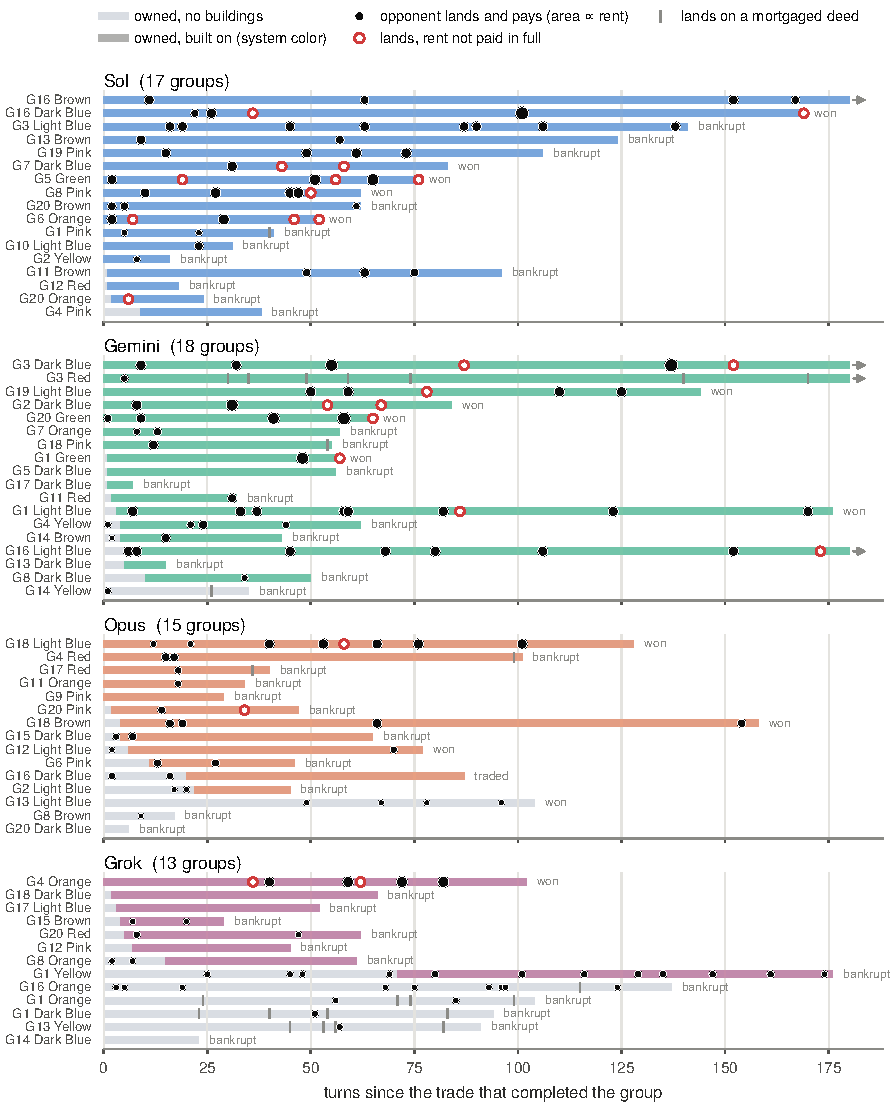
\includegraphics[width=\linewidth,height=0.80\textheight,keepaspectratio]{fig_timeline.pdf}
\caption{Every color group completed by trade, from the completing trade to the end of the episode. Rows are ordered by how soon the owner built. Episodes longer than 180 turns are clipped at the arrow. The label at the right says how the episode ended.}
\label{fig:timeline}
\end{figure}

\begin{table}[H]
\centering\small
\begin{tabular}{@{}rrrrrrrrr@{}}
\toprule
& \multicolumn{4}{c}{Sol and Gemini} & \multicolumn{4}{c}{Opus and Grok}\\
\cmidrule(lr){2-5}\cmidrule(l){6-9}
Seed block & Groups & Landings & Rent & Per landing & Groups & Landings & Rent & Per landing\\
\midrule
\BlockRentRows
\bottomrule
\end{tabular}
\caption{Rent per opponent landing on trade-completed groups, by seed block.}
\label{tab:blockrent}
\end{table}

\begin{table}[H]
\centering\small
\begin{tabular}{@{}lrrrr@{}}
\toprule
& Debt & & & Eliminated with a\\
System & episodes & Paid & Eliminated & payment route\\
\midrule
\DebtRows
\bottomrule
\end{tabular}
\caption{Debt episodes by system. Payment routes for the three eliminations in the last column are inherited.}
\label{tab:debt}
\end{table}

Of the \fact{debt.paid} payments, \fact{debt.paid-composition.mortgage-only} used mortgages only, \fact{debt.paid-composition.sales-only} building sales only and \fact{debt.paid-composition.both} both. Of the \fact{debt.eliminated} eliminations, \fact{debt.eliminated-after-some-liquidation} followed at least one liquidation action in the same episode and \fact{debt.eliminated-after-building-sale} followed a building sale. The median trade-completed group is landed on \fact{conv.trade-groups.median-landings-per-group} times. Seller outcomes in Table~\ref{tab:sellers} are stable to the building window. With a four-turn window \fact{conv.seller-conversion.sensitivity-window-4.all-one-sided.built-after-sale.seller-won} of \fact{conv.seller-conversion.sensitivity-window-4.all-one-sided.built-after-sale.n} builders and \fact{conv.seller-conversion.sensitivity-window-4.all-one-sided.no-construction-after-sale.seller-won} of \fact{conv.seller-conversion.sensitivity-window-4.all-one-sided.no-construction-after-sale.n} others won. With a twelve-turn window the counts are \fact{conv.seller-conversion.sensitivity-window-12.all-one-sided.built-after-sale.seller-won} of \fact{conv.seller-conversion.sensitivity-window-12.all-one-sided.built-after-sale.n} and \fact{conv.seller-conversion.sensitivity-window-12.all-one-sided.no-construction-after-sale.seller-won} of \fact{conv.seller-conversion.sensitivity-window-12.all-one-sided.no-construction-after-sale.n}. Among sellers with under \$100, \fact{conv.seller-conversion.sensitivity-window-4.seller-under-100.built-after-sale.seller-won} of \fact{conv.seller-conversion.sensitivity-window-4.seller-under-100.built-after-sale.n} builders won with the four-turn window and \fact{conv.seller-conversion.sensitivity-window-12.seller-under-100.built-after-sale.seller-won} of \fact{conv.seller-conversion.sensitivity-window-12.seller-under-100.built-after-sale.n} with the twelve-turn window, and no seller who did not build won under either.

\section{Estates and cohort}
\label{app:estates}

\begin{table}[H]
\centering\footnotesize
\begin{tabularx}{\linewidth}{@{}rrllrrrL{0.14\linewidth}Yl@{}}
\toprule
& & First & First & \multicolumn{3}{c}{Creditor before the estate} & Creditor's & Estate deeds &\\
\cmidrule(lr){5-7}
G & Turn & out & creditor & share & rank & rent rank & built groups & (complete groups) & Winner\\
\midrule
\EstateRows
\bottomrule
\end{tabularx}
\caption{Positions at the first liquidation menu of the debt that ends in each game's first elimination. Share and rank refer to total assets, and rent rank to rent received so far. With rent received as the measure of who was ahead, the first creditor leads in \fact{estate.first-creditor-leads-rent-received} games.}
\label{tab:estates}
\end{table}

\begin{table}[H]
\centering\small
\begin{tabular}{@{}lrrrr@{}}
\toprule
Completing acquisition & Episodes & Eventual winner & With any rent & Rent received\\
\midrule
\RouteRows
\bottomrule
\end{tabular}
\caption{How color groups were completed. Winner status comes from the same games, so the column describes concentration and no effect on winning.}
\label{tab:routes}
\end{table}

\begin{table}[H]
\centering\small
\begin{tabular}{@{}rrrrlr@{}}
\toprule
Game & Seed block & Rotation & Turns & Winner & Winner's seat\\
\midrule
\CohortRows
\bottomrule
\end{tabular}
\caption{The cohort. Seeds by block are 751774554, 2506298840, 2573692901, 3648314310 and 2766649504. Rotations are cyclic, so the four rotations of a block cover 4 of the 24 possible seat orders.}
\label{tab:cohort}
\end{table}

\section{Controls and transcript provenance}
\label{app:transcripts}

Three further exchanges limit how the incidents should be read. They are context and enter no count.

\paragraph{A false premise is corrected and the offer accepted (G19).} Grok's applied call proposes Virginia and \$150 for States, with this message.
\TranscriptQuote{g19-d135-public}
Both deeds are pink. The private note on the same response retracts the offer, and the response text names a different action, ending the turn.
\TranscriptQuote{g19-d135-note}
\TranscriptQuote{g19-d136-public}
Sol corrects the color claim and accepts the terms. Accepting an offer need not mean accepting the proposer's account of it.

\paragraph{A false completion claim is corrected and a true one is refused (G11).} Sol offers Virginia for Grok's Pennsylvania and says Virginia completes Grok's pinks. It does not, because Sol also holds St.\ Charles.
\TranscriptQuote{g11-d256-public}
\TranscriptQuote{g11-d257-public}
\TranscriptQuote{g11-d258-public}
The second offer would complete Grok's pinks, and Grok still refuses because the trade completes Sol's greens.

\paragraph{A false obstacle follows a decision already made (G3).} With one house left in the bank, Grok tells Gemini that it cannot build, while its own note says that it can.
\TranscriptQuote{g3-d363-public}
\TranscriptQuote{g3-d363-note}
\TranscriptQuote{g3-d364-note}
Gemini had already chosen to hold before the message. A false statement followed by the behavior it urges does not show that the statement was relied on.

\paragraph{How quotations are produced.} A script reads each quoted field from the canonical decision file and writes the quotation, its label and a manifest entry with the file hash, line, field pointer, character span and field hash. No quotation is typed by hand. A label names the speaker, the channel, the game, the zero-based decision and the selected attempt, and says whether the card shows the full field or an excerpt. Bracketed ellipses mark omitted text. Errors in quotations are left as written. There are four channels. A public message and a private note are fields of the applied action. Assistant content is the text returned beside a tool call. The returned provider explanation is the provider's reasoning field. For public messages addressed to a counterparty, the manifest records the first later prompt of that player that contains the message. Of the \fact{d.quotes.cards} quotation cards, \fact{d.quotes.reused} repeat definitions checked in the earlier paper and match them character for character.

\section{Reproducibility, research assistance and authorship}
\label{app:repro}

The code and the twenty saved games are public at \url{https://github.com/KushagraBharti/MonopolyBench}. This draft is a later local artifact. It changes no game record, prompt, engine file or earlier manuscript, and it ran no game, engine call, replay or model call. Every table, figure, quotation and number in the text is generated by the scripts in the draft's \texttt{analysis} directory from the saved games and from the earlier ledgers named in Table~\ref{tab:reconcile}. A build fails if the text cites a number that the scripts do not produce.

The project uses LLM research assistants under human direction. In this round four assistants each wrote a complete paper independently before any cross-review. This draft was written by one of them, Claude Fable 5.2, which shares a developer with the evaluated Opus system. The assistant chose the analyses, the incidents and the framing after reading the records and the earlier reviews. The two semantic readings cited in Section~\ref{sec:attention} came from other assistant instances in earlier work. No human labeled any record for this paper, and no assistant is an author. The human author line is the project owner's decision.

\end{document}
